\begin{document}
\part{Hardware de Computación Cuántica}




\chapter{Breve introducción sobre Hardware de Computación Cuántica}

En este capitulo vamos a ver un poco sobre diferentes implementaciones de ordenadores cuánticos.

\section{Modelos de Computación Cuántica}

Independientemente del hardware que haya debajo, los ordenadores cuánticos pueden clasificarse en tres categorías:
\begin{itemize}
	\item Ordenadores Cuánticos \textbf{Fault Tolerant}: Estos ordenadores presentan dos capas de abstracción: corrección de errores + puertas. El nombre ``Fault Tolerant'' se refiere a que son ordenadores resistentes a errores. Son el objetivo a conseguir.
	\item Ordenadores Cuánticos \textbf{NISQ}: Estos ordenadores presentan una capa de abstracción: puertas. ``NISQ" son las iniciales de Noisy Intermediate Scale Quantum, que se refiere a que son ordenadores con errores (ruido), lo que limita su aplicación. Son los ordenadores de puertas que tenemos actualmente.
	\item Ordenadores Cuánticos \textbf{analógicos}: Estos ordenadores no presentan ninguna capa de abstracción: se hace evolucionar un sistema cuántico real. Son los ordenadores de \textbf{Anneling}.
\end{itemize}



\subsection{Computación Cuántica Analógica}

Los ordenadores cuánticos analógicos son los que se usan en Quantum Anneling.

\begin{itemize}
\item \textbf{¿Qué hacen?}: Aplicar parámetros de control para hacer evolucionar en el tiempo un sistema cuántico del mundo real.

\item \textbf{Casos de uso}: Simulación cuántica (abierta y cerrada), Optimización.

\item \textbf{Argumentos a favor}: Uso muy eficiente de los recursos de hardware cuántico. Muy rápidos (sin capas de abstracción)

\item \textbf{Argumentos en contra}: Alta especialización para aplicaciones especificas. El ruido del hardware puede ser limitante
\end{itemize}


\subsection{Computación basada en puertas NISQ}

Los ordenadores basados en puertas NISQ (Noisy Intermediate Scale Quantum) son los ordenadores basados en puertas que tenemos a día de hoy. En estos, hay que lidiar con el \textbf{ruido} y con tiempos de coherencia relativamente pequeños. Esto limita en gran medida el uso que se le puede dar a estos ordenadores, con lo que los estudios se centran en dos cosas: en el desarrollo de ordenadores Fault-Tolerant y en ver que problemas se pueden resolver a pesar de los problemas de estos ordenadores. Por ejemplo, los algoritmos cuánticos variacionales se pensaron para poder sacar partido a estos ordenadores.


\begin{itemize}
\item \textbf{¿Qué hacen?}: Aplicar puertas cuánticas imperfectas para implementar una computación cuántica universal ruidosa. (Nota: suelen incluir puertas de rotación arbitraria.)

\item \textbf{Casos de uso}: Simulación cuántica (cerrada), algoritmos cuánticos variacionales, machine learning cuántico

\item \textbf{Argumentos a favor}: Son flexibles (muchos tipos de implementaciones) y rápidos (una capa de abstracción: las puertas).

\item \textbf{Argumentos en contra}: El ruido es limitante y no se tiene claro como extender el tiempo de coherencia de los qubits.

\end{itemize}



\subsection{Computación basada en puertas Fault-Tolerant}


Los ordenadores basados en puertas tolerantes a fallos (Fault-Tolerant) son el objetivo a conseguir. Serían ordenadores universales en los que se podrían ejecutar circuitos cuánticos con toda la profundidad que se quiera.

\begin{itemize}
\item \textbf{¿Qué hacen?}: Aplicar puertas cuánticas con corrección de errores para implementar una computación cuántica universal perfecta. (Nota: un conjunto de puertas restrictivo (por ejemplo, Clifford+T)).

\item \textbf{Casos de uso}: Simulación cuántica (alta precisión), Factorización, Sistemas lineales, Sistemas no lineales.

\item \textbf{Argumentos a favor}: Algoritmos fiables con pruebas. La Corrección Cuántica de Errores (QEC) permite ir más allá del límite del tiempo de coherencia de los qubits.

\item \textbf{Argumentos en contra}: Requieren \textbf{muchos} qubits físicos. Los algoritmos requieren muchas puertas (>$10^6$). Lento, los gastos generales de QEC llevan tiempo (2 capas de abstracción).

\end{itemize}


\subsection{Tres tipos de ordenadores cuánticos comerciales}

En la Fig. \ref{Fig_Hardware_ordenadores_comerciales} podemos ver las apuestas de diferentes empresas para el desarrollo de ordenadores cuánticos de diferentes tecnologías.

	\begin{figure}[t]
	\centering 
	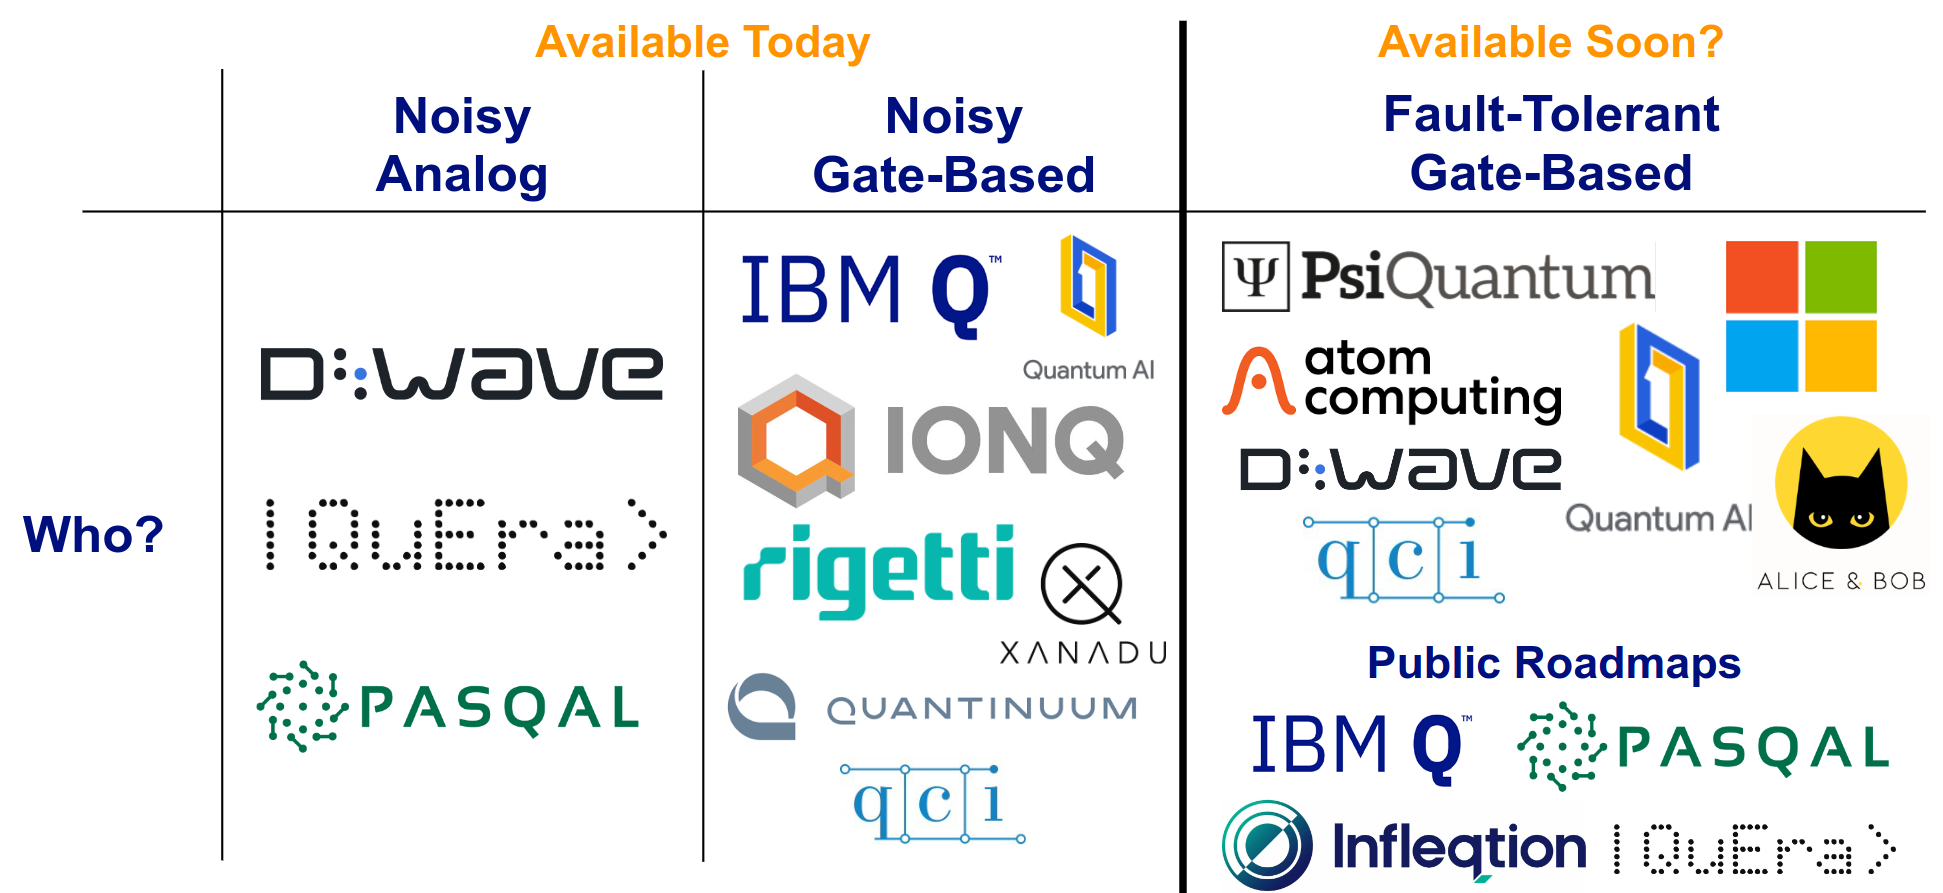
\includegraphics[width=1\linewidth]{Figuras/Fig_Hardware_ordenadores_comerciales.png}
	\caption{Ordenadores cuánticos comerciales}
	\label{Fig_Hardware_ordenadores_comerciales}
	\end{figure}









\section{Estructura del Hardware de un Ordenador Cuántico}

Dado que un ordenador cuántico debe interactuar con usuarios, datos y redes (tareas en las que destaca la informática convencional), un ordenador cuántico puede aprovechar un \textbf{ordenador convencional} para estas tareas siempre que sea más eficiente hacerlo. Además, los sistemas qubit requieren un control cuidadosamente orquestado para funcionar de forma útil; este control puede gestionarse mediante ordenadores convencionales.

Para ayudar a conceptualizar los componentes de hardware necesarios para un ordenador cuántico analógico o basado en compuertas, el hardware puede modelarse en cuatro capas abstractas: 
\begin{itemize}
\item El "plano de datos cuánticos", donde residen los qubits.
\item El "plano de control y medición", responsable de realizar operaciones y mediciones en los qubits según sea necesario.
\item El "plano del procesador de control", que determina la secuencia de operaciones y mediciones que requiere el algoritmo, utilizando potencialmente los resultados de las mediciones para informar de las operaciones cuánticas posteriores.
\item El ``procesador anfitrión (host)", un ordenador clásico que gestiona el acceso a redes, grandes matrices de almacenamiento e interfaces de usuario. Este procesador host ejecuta un sistema operativo/interfaz de usuario convencional, que facilita las interacciones de los usuarios, y dispone de una conexión de gran ancho de banda con el procesador de control.
\end{itemize}

Esta sección se basa en el capítulo 5 de \cite{bib_hardware_intro_progress_and_prospects}.


	\subsection{Plano de datos cuánticos (Quantum Data Plane)}
	
El plano de datos cuánticos es el ``corazón'' de un Computador Cuántico. Incluye los \textbf{qubits físicos} y las estructuras necesarias para mantenerlos en su lugar. También debe contener cualquier \textbf{circuito de apoyo necesario para medir} el estado de los qubits y \textbf{realizar operaciones de puerta} en los qubits físicos para un sistema basado en puertas o \textbf{controlar el Hamiltoniano} para un ordenador analógico.  En el caso de los sistemas basados en puertas, como algunas operaciones con qubits requieren dos qubits, el plano de datos cuánticos debe proporcionar una \textbf{red de ``cableado'' que permita interactuar a dos o más qubits}. Los sistemas analógicos suelen requerir una comunicación más rica entre los qubits, que debe ser soportada por esta capa.


La alta fidelidad de los qubits requiere un fuerte aislamiento del entorno, lo que tiene el efecto de limitar la conectividad (puede que no sea posible que todos los qubits interactúen directamente con todos los demás qubits), por lo que el cálculo debe ajustarse a las restricciones arquitectónicas específicas de esta capa. Estas restricciones significan que tanto la \textbf{fidelidad} de la operación como la \textbf{conectividad} son métricas importantes de la capa de datos cuánticos.	
	

A diferencia de un ordenador clásico, en el que tanto los componentes del plano de control como los del plano de datos utilizan la misma tecnología de silicio y están integrados en el mismo dispositivo, el control del plano de datos cuántico requiere una tecnología distinta de la de los qubits, y se realiza externamente mediante una capa separada de control y medición. 

La información de control de los qubits, de naturaleza analógica, debe enviarse al qubit (o qubits) correcto. En algunos sistemas, esta información de control se transmite eléctricamente mediante cables, por lo que éstos forman parte del plano de datos cuánticos; en otros, se transmite con radiación óptica o de microondas. La transmisión debe implementarse de manera que tenga una alta especificidad, de modo que afecte sólo al qubit o qubits deseados, sin perturbar a los demás qubits del sistema. Esto resulta cada vez más difícil a medida que aumenta el número de qubits; El número de qubits de un módulo es, por tanto, otro parámetro importante de una capa de datos cuántica.

Es decir, las propiedades clave que definen la calidad de un plano de datos cuántico son la \textbf{tasa de error de las puertas de un qubit y de dos qubits}, la \textbf{conectividad} interqubit, los \textbf{tiempos de coherencia} de los qubits y el \textbf{número de qubits} que puede contener un módulo.


	\subsection{Plano de control y medida}

El plano de control y medición \textbf{convierte las señales digitales del procesador de control, que indica qué operaciones cuánticas deben realizarse, en las señales de control analógicas necesarias para realizar las operaciones en los qubits del plano de datos cuánticos}. También \textbf{convierte la salida analógica de las mediciones de los qubits} en el plano de datos\textbf{ en datos binarios} clásicos que el procesador de control puede manejar. 

La generación y transmisión de señales de control es un reto debido a la naturaleza analógica de las puertas cuánticas; pequeños errores en las señales de control, o irregularidades en el diseño físico del qubit, afectarán a los resultados de las operaciones. Los errores asociados a cada operación de puerta se acumulan a medida que la máquina funciona. 

Cualquier imperfección en el aislamiento de estas señales (lo que se denomina interferencia (\textbf{crosstalk}) de señales) hará que aparezcan pequeñas señales de control para qubits que, de otro modo, no deberían dirigirse durante una operación, lo que provocará pequeños errores en su estado de qubit. Cabe señalar que la interferencia puede producirse directamente entre los propios qubits en el plano de datos cuánticos.

Afortunadamente, tanto los errores de fabricación del qubit como los errores de interferencia de la señal son sistemáticos y cambian lentamente con la configuración mecánica del sistema. Los efectos de estos errores que cambian lentamente pueden minimizarse utilizando formas de impulsos de control que reduzcan la dependencia del qubit de estos factores, y mediante la \textbf{calibración periódica del sistema}, siempre que exista un mecanismo para medir estos errores y un software que ajuste las señales de control para reducir estos errores a cero (calibración del sistema). Dado que cada señal de control puede interactuar potencialmente con cualquier otra señal de control, el número de mediciones y cálculos necesarios para lograr esta calibración se duplica con creces a medida que se duplica el número de qubits del sistema.

La naturaleza de las señales de control de un ordenador cuántica depende de la tecnología de qubits subyacente. Por ejemplo, los sistemas que utilizan qubits de iones atrapados suelen basarse en señales de microondas u ópticas (formas de radiación electromagnética) transmitidas a través del espacio libre o de guías de ondas y enviadas a la ubicación de los qubits. Los sistemas de qubits superconductores se controlan mediante microondas y señales eléctricas de baja frecuencia, ambas comunicadas a través de cables que se introducen en un aparato de refrigeración para llegar a los qubits dentro del entorno controlado.

A diferencia de las puertas clásicas, inmunes al ruido y con tasas de error despreciables, las operaciones cuánticas dependen de la precisión con la que se suministran las señales de control y tienen tasas de error no despreciables. 

Como ninguna puerta cuántica puede ser más rápida que el pulso de control que la implementa, aunque el sistema cuántico permita en principio un funcionamiento ultrarrápido, la velocidad de la puerta estará limitada por el tiempo necesario para construir y transmitir un pulso de control extremadamente preciso. Afortunadamente, la velocidad de la tecnología de silicio actual es lo suficientemente rápida como para que \textbf{la velocidad de la puerta esté limitada por el plano de datos cuánticos}, y no por el plano de control y medición. Actualmente, esta velocidad de puerta permite tiempos de aplicación de  decenas a cientos de nanosegundos para los qubits superconductores y de uno a cien microsegundos para los qubits de iones atrapados.



	
	\subsection{Plano del procesador de control}

El plano del procesador de control \textbf{identifica y activa} \textbf{la secuencia de operaciones y mediciones de las puertas cuánticas} o el Hamiltoniano adecuado (que posteriormente son llevadas a cabo por el plano de control y medición en el plano de datos cuánticos). Estas secuencias ejecutan el programa, proporcionado por el procesador anfitrión, para implementar un algoritmo cuántico. Las herramientas de software deben adaptar los programas a las capacidades específicas de la capa cuántica.

Una de las tareas más importantes y desafiantes del plano del procesador de control será \textbf{ejecutar el algoritmo cuántico de corrección de errores} (si es posible). Se requiere un procesamiento de información clásico significativo para calcular las operaciones cuánticas necesarias para corregir errores basándose en los resultados del síndrome medido, y el tiempo necesario para este procesamiento puede ralentizar el funcionamiento del ordenador cuántico. 

Construir un plano del procesador de control para grandes máquinas cuánticas es un reto y un área activa de investigación. Un enfoque divide el plano en dos partes:
\begin{itemize}
\item La primera es simplemente un procesador clásico que ``ejecuta'' el programa cuántico.
\item La segunda parte es un bloque de hardware personalizado escalable que interactúa directamente con el plano de control y medición, y combina las ``instrucciones'' de nivel superior emitidas por el controlador principal con las mediciones del síndrome (corrección de errores) para calcular las siguientes operaciones que deben realizarse en los qubits.
\end{itemize}
El reto consiste en crear un hardware personalizado escalable que sea lo suficientemente rápido y pueda ampliarse con el tamaño de la máquina, y en crear la abstracción de instrucciones de alto nivel adecuada.

El plano del procesador de control opera a un bajo nivel de abstracción: convierte el código compilado en órdenes para la capa de control y medición. Como resultado, un usuario no interactuará con (ni necesitará entender) el plano del procesador de control directamente. En su lugar, el usuario interactuará con un \textbf{ordenador anfitrión (host computer)}. Este plano se conectará a ese ordenador y actuará para acelerar la ejecución de algunas aplicaciones.  Estos aceleradores suelen tener una conexión de gran ancho de banda con el procesador anfitrión, normalmente a través de un acceso compartido a parte de la memoria del procesador anfitrión, que puede utilizarse para transferir tanto el programa que debe ejecutar el procesador de control como los datos que debe utilizar durante la ejecución.


	\subsection{Plano del procesador anfitrión (host processor)}



El procesador anfitrión es un \textbf{ordenador clásico, que ejecuta un sistema operativo convencional} con bibliotecas de soporte estándar para su propio funcionamiento. Este sistema informático proporciona todas las herramientas de desarrollo de software y los servicios que los usuarios esperan de un sistema informático. Ejecutará las herramientas de desarrollo de software necesarias para crear aplicaciones que se ejecutarán en el procesador de control, que son diferentes de las que se utilizan para controlar los ordenadores clásicos actuales, además de proporcionar los servicios de almacenamiento y redes que una aplicación cuántica pueda necesitar mientras se ejecuta. Adjuntar un procesador cuántico a un ordenador clásico permite utilizar todas sus funciones sin necesidad de empezar completamente de cero.

\begin{mybox_blue}{Nota: QPUs como GPUs en cálculo}
Es bien conocido que las GPUs o tarjetas gráficas, aparte de usarse para renderizar gráficos, se usan también para cálculo (como para entrenar IAs). De esta formas, las GPUs se usan como \textbf{aceleradores}, en el sentido de que un ordenador funcionan usando una CPU normal y delega ciertos cálculos en GPU. 
\vspace{0.3cm}

El enfoque de los QPUs o procesadores cuánticos es similar. Un ordenador clásico normal con una CPU normal es el que hace todo lo esperable por parte de un ordenador, solo que tiene la opción de mandar algún cálculo concreto a ejecutarse en un QPU, recogiendo los resultados y procesandolos.
\end{mybox_blue}


\section{Tipos de Tecnologías de qubits.}



En la Fig. \ref{Fig_Hardware_qubit_tecnologies} podemos ver el estado del arte (hasta enero de 2022) de las diferentes tecnologías de qubits. En esta sección vamos a hacer un pequeño resumen de algunas de las más importantes. 

	\begin{figure}[H]
	\centering 
	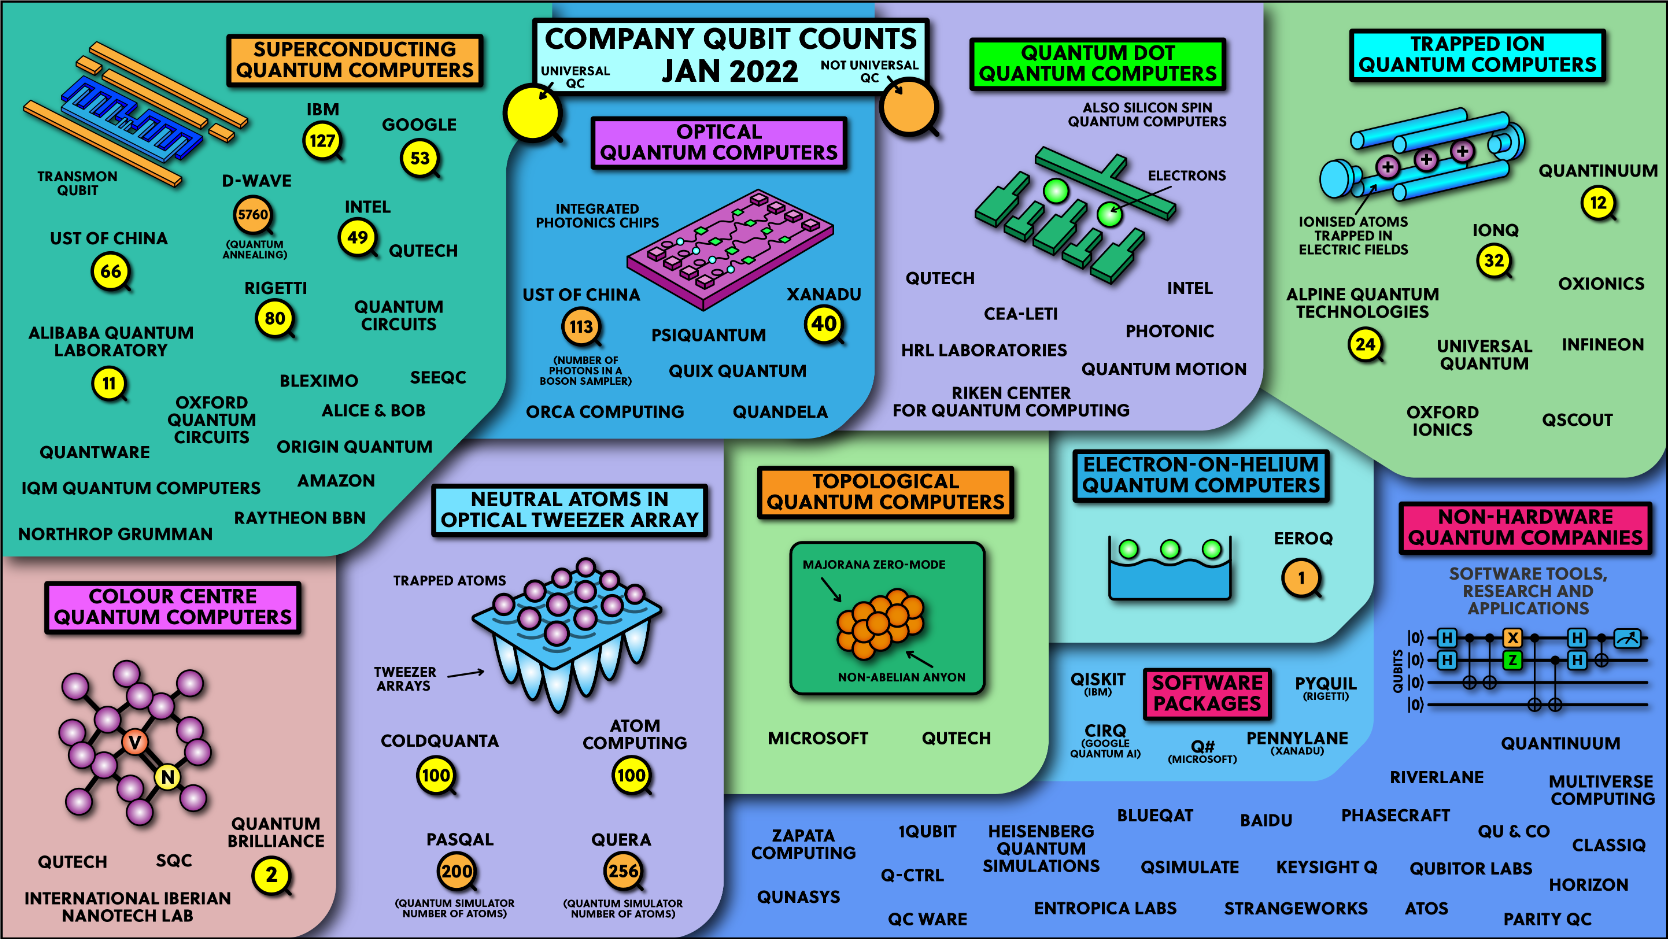
\includegraphics[width=1\linewidth]{Figuras/Fig_Hardware_qubit_tecnologies.png}
	\caption{Diferentes tecnologías de qubits de diferentes empresas, con su número máximo de qubits (hasta enero de 2022). Los números en \textbf{amarillo} representan ordenadores universales y los \textbf{naranjas} ordenadores no-universales. Figura tomada del vídeo \href{https://www.youtube.com/watch?v=gcbMKt079l8}{Who Has The Best Quantum Computer?} }
	\label{Fig_Hardware_qubit_tecnologies}
	\end{figure}


	\subsection{Criterio de Divicenzo} \label{sec_criterio_divicenzo}

Para poder implementar de forma satisfactoria un ordenador cuántico, el montaje experimental (el ordenador cuántico) debe satisfacer las siete condiciones del criterio de DiVincenzo \cite{bib_DiVincenzo_2000}. Las cinco primeras son para ordenadores cuánticos:    
\begin{itemize}
\item (a) Los qubits deben estar bien caracterizados y ser fáciles de producir. (b) El sistema debe ser escalable, es decir, debe poder gestionar un número arbitrario de qubits.

\item La capacidad de inicializar el estado de los qubits a un estado fiducial simple, como por ejemplo $\ket{00\dots}$.

\item Tiempos de decoherencia relevantes largos, mucho más largos que el tiempo de funcionamiento de la puerta. Es decir, un qubit debe ser estable en escalas de tiempo mayores que el tiempo típico necesario para operar con él.

\item Debe de ser posible implementar un conjunto universal de puertas.
\item Debe existir un procedimiento fiable para leer el estado de cada qubit por separado.
\end{itemize}

Los dos restantes son necesarios para la comunicación cuántica:
\begin{itemize}
	\item La capacidad de interconvertir qubits estacionarios y voladores.
	\item La capacidad de transmitir fielmente qubits voladores entre ubicaciones específicas.
\end{itemize}
    
    
	
	\subsection{Iones Atrapados (Trapped Ion Qubits)}


La primera puerta lógica cuántica se demostró en 1995 utilizando iones atómicos atrapados \cite{bib_PhysRevLett.75.4714}, tras una propuesta teórica de ese mismo año \cite{bib_PhysRevLett.74.4091}. Desde la demostración original, los avances técnicos en el control de qubits han permitido la demostración experimental de procesadores totalmente funcionales a pequeña escala y la implementación de una amplia gama de algoritmos cuánticos sencillos.

A pesar del éxito de las demostraciones a pequeña escala, la tarea de construir ordenadores cuánticos escalables y considerados viables según los estándares actuales de la industria informática a partir de iones atrapados sigue siendo un reto importante.  La construcción de un ordenador cuántico basado en qubits de iones atrapados requiere la integración de tecnologías de una amplia gama de dominios, incluidos los sistemas de vacío, láser y ópticos, la tecnología de radiofrecuencia (RF) y microondas, y los controladores electrónicos coherentes. El camino hacia un ordenador cuántico viable debe abordar estos retos de integración.

Un plano de datos cuánticos de iones atrapados comprende los iones que sirven de qubits y una ``trampa'' que los mantiene en lugares específicos. El plano de control y medición incluye una fuente láser (o de microondas) muy precisa que puede dirigirse a un ion específico para afectar a su estado cuántico, otro láser para "enfriar" y permitir la medición de los iones, y un conjunto de detectores de fotones para "medir" el estado de los iones mediante la detección de los fotones que dispersan.

Para más información sobre esta tecnología, consultar el Capitulo \ref{sec_chapter_hw_iones}.

	\subsection{Qubits Superconductores}

Al igual que los actuales circuitos integrados de silicio, los qubits superconductores son circuitos electrónicos definidos litográficamente. Cuando se enfrían a temperaturas de mili-Kelvin, presentan niveles de energía cuantizados (debido a estados cuantizados de carga electrónica o flujo magnético, por ejemplo), por lo que a veces se les denomina "átomos artificiales". 

Su compatibilidad con la electrónica de control de microondas, su capacidad para operar en escalas de tiempo de nanosegundos, la mejora continua de los tiempos de coherencia y el potencial para aprovechar la escala litográfica, convergen para situar a los qubits superconductores en la vanguardia de las modalidades de qubits que se están considerando tanto para la computación cuántica digital como para el anneling cuántico. 

Para más información sobre esta tecnología, consultar el Capitulo \ref{sec_chapter_hw_scq}.

	\subsection{Computación cuántica con fotones}

Los fotones tienen una serie de propiedades que los convierten en una tecnología atractiva para los ordenadores cuánticos: son partículas cuánticas que interactúan débilmente con su entorno y entre sí. Este aislamiento natural del entorno los convierte en un enfoque obvio para la comunicación cuántica. Esta utilidad básica para la comunicación, combinada con excelentes puertas de un solo qubit de alta fidelidad, hace que muchos de los primeros experimentos cuánticos se realizaran con fotones. 

Un reto clave de los ordenadores cuánticos fotónicos es cómo crear puertas robustas de dos qubits. Los investigadores trabajan actualmente en dos enfoques para este problema. 
\begin{itemize}
\item En la \textbf{computación cuántica de óptica lineal}, se crea una interacción fuerte efectiva mediante una combinación de operaciones y mediciones monofotónicas, que puede utilizarse para implementar una puerta probabilística de dos qubits, que anuncia cuándo ha tenido éxito. 
\item Un segundo enfoque utiliza pequeñas estructuras en cristales semiconductores para la interacción de fotones, y también puede considerarse un tipo de ordenador cuántico semiconductor. Estas estructuras pueden ser naturales, llamadas \textbf{``defectos ópticamente activos''}, o artificiales, que suelen ser una estructura llamada \textbf{``quantum dot''}.
\end{itemize}

Los trabajos para construir ordenadores fotónicos lineales a pequeña escala han tenido éxito, y hay varios grupos que intentan aumentar el tamaño de estas máquinas. Uno de los principales problemas es el ``tamaño'' del qubit fotónico. Dado que los fotones utilizados en la computación cuántica fotónica suelen tener longitudes de onda de alrededor de una micra, y que los fotones se mueven a la velocidad de la luz y suelen dirigirse a lo largo de una dimensión del chip óptico, aumentar el número de fotones, y por tanto el número de qubits, hasta cifras extremadamente grandes en un dispositivo fotónico es aún más difícil que en sistemas con qubits que pueden localizarse en el espacio. Sin embargo, se espera que sea posible crear matrices con muchos miles de qubits. 

	\subsection{Qubits con semiconductores}
	
Los qubits semiconductores pueden dividirse en dos tipos según utilicen fotones o señales eléctricas para controlar los qubits y sus interacciones. 
\begin{itemize}
\item Los qubits semiconductores controlados ópticamente suelen utilizar \textbf{defectos ópticamente activos} o \textbf{quantum dots} que inducen fuertes acoplamientos efectivos entre fotones.

El escalado de los qubits con puertas óptica requiere una mejor uniformidad y la eliminación de la necesidad de tratar ópticamente cada qubit de forma individual.

\item Los qubits semiconductores controlados eléctricamente utilizan voltajes aplicados a puertas metálicas definidas litográficamente para confinar y manipular los electrones que forman los qubits. Este enfoque es más similar al utilizado en la electrónica clásica actual, lo que podría permitir que las grandes inversiones que han hecho posible la enorme escalabilidad de la electrónica clásica faciliten el escalado de los procesadores de información cuántica. 

Los qubits con activación eléctrica son potencialmente muy densos. Aunque la alta densidad puede permitir integrar un gran número de qubits en el chip, agrava el problema de construir un plano de control y medición para este tipo de qubits: proporcionar el cableado necesario y evitar al mismo tiempo interferencias entre las señales de control será extremadamente difícil.
\end{itemize} 



  
  


	\subsection{Qubits con átomos neutros}
	
Los átomos neutros son otro método para crear qubits muy similar al de los iones atrapados, pero en lugar de utilizar átomos ionizados y aprovechar su carga para mantener los qubits en su sitio, se emplean átomos neutros y pinzas láser. Al igual que los qubits de iones atrapados, se utilizan pulsos ópticos y de microondas para manipular los qubits, y también se emplean láseres para enfriar los átomos antes del cálculo.

Gracias a los recientes avances en la tecnología de pinzas ópticas, los átomos neutros pueden utilizarse como qubits robustos y versátiles. En 2022, una colaboración entre QuEra y varias instituciones académicas produjo un dispositivo de átomos neutros con 256 qubits \cite{bib_hw_QuEra_aquila} (analógico, no de puertas). En el sector privado esta tecnología es usada por empresas emergentes como Pasqal, QuEra y Atom Computing. 

En la computación cuántica con átomos neutros se usan \textbf{átomos de Rydberg}. Un átomo de Rydberg es un átomo excitado con uno o más electrones que tienen un número cuántico principal, $n$, muy alto. Cuanto mayor es el valor de $n$, más lejos está el electrón del núcleo, por término medio. Los átomos de Rydberg tienen una serie de propiedades peculiares, como una gran sensibilidad a los campos eléctricos y magnéticos, largos periodos de desintegración y funciones de onda de los electrones que se aproximan, en algunas condiciones, a las órbitas clásicas de los electrones alrededor de los núcleos. Los electrones del núcleo protegen al electrón exterior del campo eléctrico del núcleo, de forma que, desde la distancia, el potencial eléctrico parece idéntico al que experimenta el electrón en un átomo de hidrógeno.

		\subsection{Qubits topológicos}

El último enfoque de la computación cuántica que vamos a ver es el que utiliza qubits topológicos. 

La topología es la rama de las matemáticas que se ocupa de las propiedades de un objeto geométrico que se conservan bajo deformaciones continuas, como estirarse, retorcerse, arrugarse y doblarse; es decir, sin cerrarse agujeros, abrirse huecos, rasgarse, pegarse o atravesarse. 

Un ejemplo clásico es que una taza y una rosquilla (técnicamente, un toroide) son topológicamente equivalente, pues los dos presentan un agujero (en la taza, es el del asa). Es decir, desde un punto de vista geométrico, una taza y una rosquilla son objetos muy diferentes, mientras que desde un punto de vista topológico, son el mismo (ver Fig. \ref{Fig_hw_map_of_tqc}).

Otro ejemplo son una cinta de papel y una banda de Möbius (ver Fig. \ref{Fig_hw_map_of_tqc}). A primera vista parecen similares (por ejemplo, solo tiene un agujero), pero topológicamente son diferentes, pues un cinta de papel tiene dos lados y la banda de Möbius solo tiene uno. Es decir, no podemos deformar de forma continua uno de ellos para convertirlo en el otro.

Pensando por ejemplo en la banda de Möbius, podemos hacerla con una tira de papel y un celo. Podemos coger ahora con la manos esta banda y deformarla, en el sentido de estirar desde dos extremos, darle la vuelta,.... Estas deformaciones cambian la forma o la posición de la banda, pero mientras sean lo suficientemente débiles como para no romperla, \textbf{no cambian sus propiedades topolígicas}. Pasa lo mismo con, por ejemplo, una bandera. Cuando le da el viento la bandera ondula, se deforma, se enrolla sobre si misma, ..., pero topológicamante sigue siendo un plano (a no ser que algo la desgarre). Es decir, las propiedades topológicas están protegidas ante deformaciones suaves. 

Los qubits topológicos usan estados topológicos. Estos qubits están protegidos de forma natural de la decoherencia por las propiedades topológicas. Además, las operaciones sobre los qubits físicos tienen fidelidades extremadamente altas porque están protegidas por la simetría topológica implementada a nivel microscópico: la corrección de errores la realiza el propio qubit. Esto reducirá y posiblemente eliminará la sobrecarga de realizar una corrección de errores cuántica explícita. 

En el planteamiento de los qubits topológicos se usan las denominadas \textbf{partículas de Majorana}. Las particulas de Majorana son teóricas, en el sentido de que nunca se han observado así que no se sabe si existen o no. Sin embargo, bajo ciertas condiciones un material puede presentar un comportamiento colectivo que se identifica con una \textbf{cuasiparticula} que presenta las propiedades de una partícula de Majorana. El término cuasipaticula hace referencia a que no es una partícula de verdad, sino un comportamiento colectivo que se comporta como un partícula (como los huecos de electrones en un material). Es decir, una cuasipartícula es una propiedad emergente. Lo que se intenta usar en computación cuántica son estas cuasipartículas de Majorana.

Aunque sería un avance asombroso, los qubits topológicos son la plataforma tecnológica menos desarrollada, hasta el punto de ser prácticamente teóricos. Hay que dar muchos pasos no triviales para demostrar la existencia de un qubit topológico, incluida la observación experimental de la estructura básica que subyace a estos qubits (los modos cero de Majorana). Una vez que estas estructuras se construyan y controlen en el laboratorio, las propiedades de resistencia a errores de este enfoque podrían permitirle escalar más rápido que los otros enfoques.

En el mundo de las grandes empresas, Microsoft está haciendo una gran apuesta por esta tecnología. En 2023, investigadores de Microsoft publicaron un artículo en Physical Review que describía un nuevo dispositivo que puede representar un qubit lógico con estabilidad de hardware, midiendo una fase de la materia consistente con la observación de la superconductividad topológica y los modos cero de Majorana \cite{bib_hw_topological_microsoft}.

Para más información sobre qubits topológicos puede verse el video de YouTube \href{https://www.youtube.com/watch?v=ihZXl33t8So}{The Radical Map of Topological Quantum Computing}, del youtuber Domain of Science.

	\begin{figure}[H]
	\centering 
	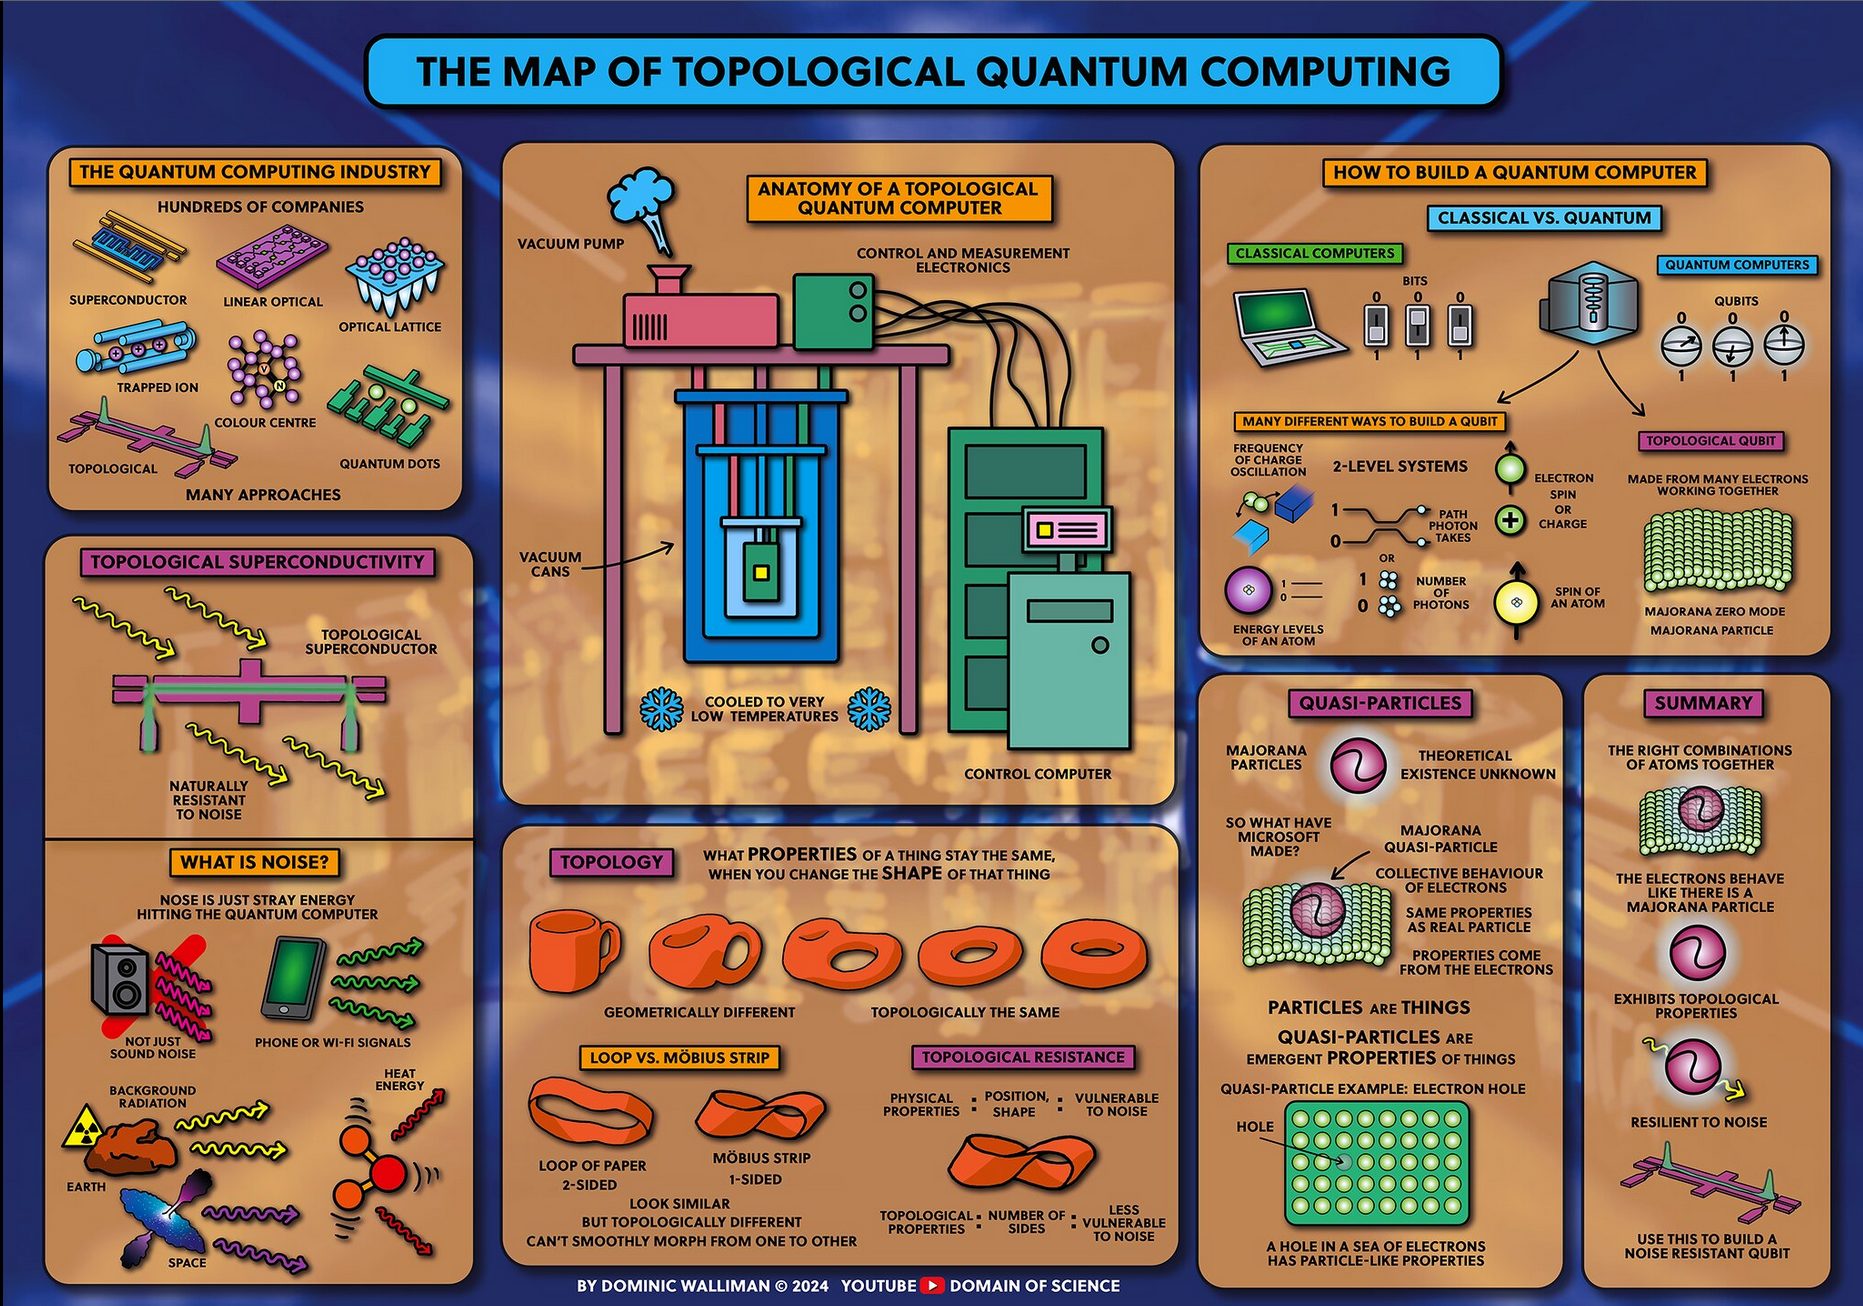
\includegraphics[width=1\linewidth]{Figuras/Fig_hw_map_of_tqc.png}
	\caption{Resumen de Computación Cuántica con Qubits topológicos de Dominuc Walliman. Figura toma del vídeo \href{https://www.youtube.com/watch?v=ihZXl33t8So}{The Radical Map of Topological Quantum Computing}}
	\label{Fig_hw_map_of_tqc}
	\end{figure}


\Ejercicio{
Buscar los chips más punteros de las principales empresas de cada tipo de tecnología de qubit (un par de empresas como mucho por tecnología).
}

\Ejercicio{
Pequeño trabajo (un par de carillas como mucho) sobre alguna tecnología de qubits que no sean superconductores o iones atrapados. Citar todas las fuentes de información usadas.
}

\section{Pulso de microondas}

A lo largo de los siguientes capítulos se va usar bastante el concepto de \textbf{pulso de frecuencia} $\omega$ (en concreto, en el rango de las microondas). Lo importante para entender estos capítulos es tener en cuenta que cuando hablamos de un pulso hablamos de un \textbf{pulso electromagnético}, es decir, de una onda electromagnética de una cierta frecuencia $\omega$. Las ondas electromagnéticas están compuestas de \textbf{fotones} (al igual que la luz, pues esta no es más que una onda electromagnética en un rango de frecuencias que podemos ver con nuestros ojos). 

El concepto clave aquí es que estos fotones son \textbf{cuantos de energía} (paquetitos de energía), y estos cuantos tiene una energía muy concreta que depende de la frecuencia de la onda electromagnética:
	\begin{equation} \label{ec_HW_E_hbar_omega}
	E = \hbar \omega \, .
	\end{equation}
donde $\hbar$ es la constante de Plack y $\omega$ es la frecuencia de la onda.

Es decir, un pulso (onda electromagnética) de frecuencia $\omega$ va estar compuesta de fotones con energía $\hbar \omega$. Si cambiamos la frecuencia del pulso, cambiamos la energía de los fotoness que lo componen. 

A lo largo los capítulos se usará el hecho de que si tenemos un sistema cuántico con varios niveles de energía, podemos hacer que el sistema pase de estar en un nivel de energía a estar en el siguiente, si le mandamos fotones con la energía \textbf{exacta} de la transición, es decir, con un pulso con una frecuencia muy concreta. 

    \begin{figure}[t]
      \centering 
      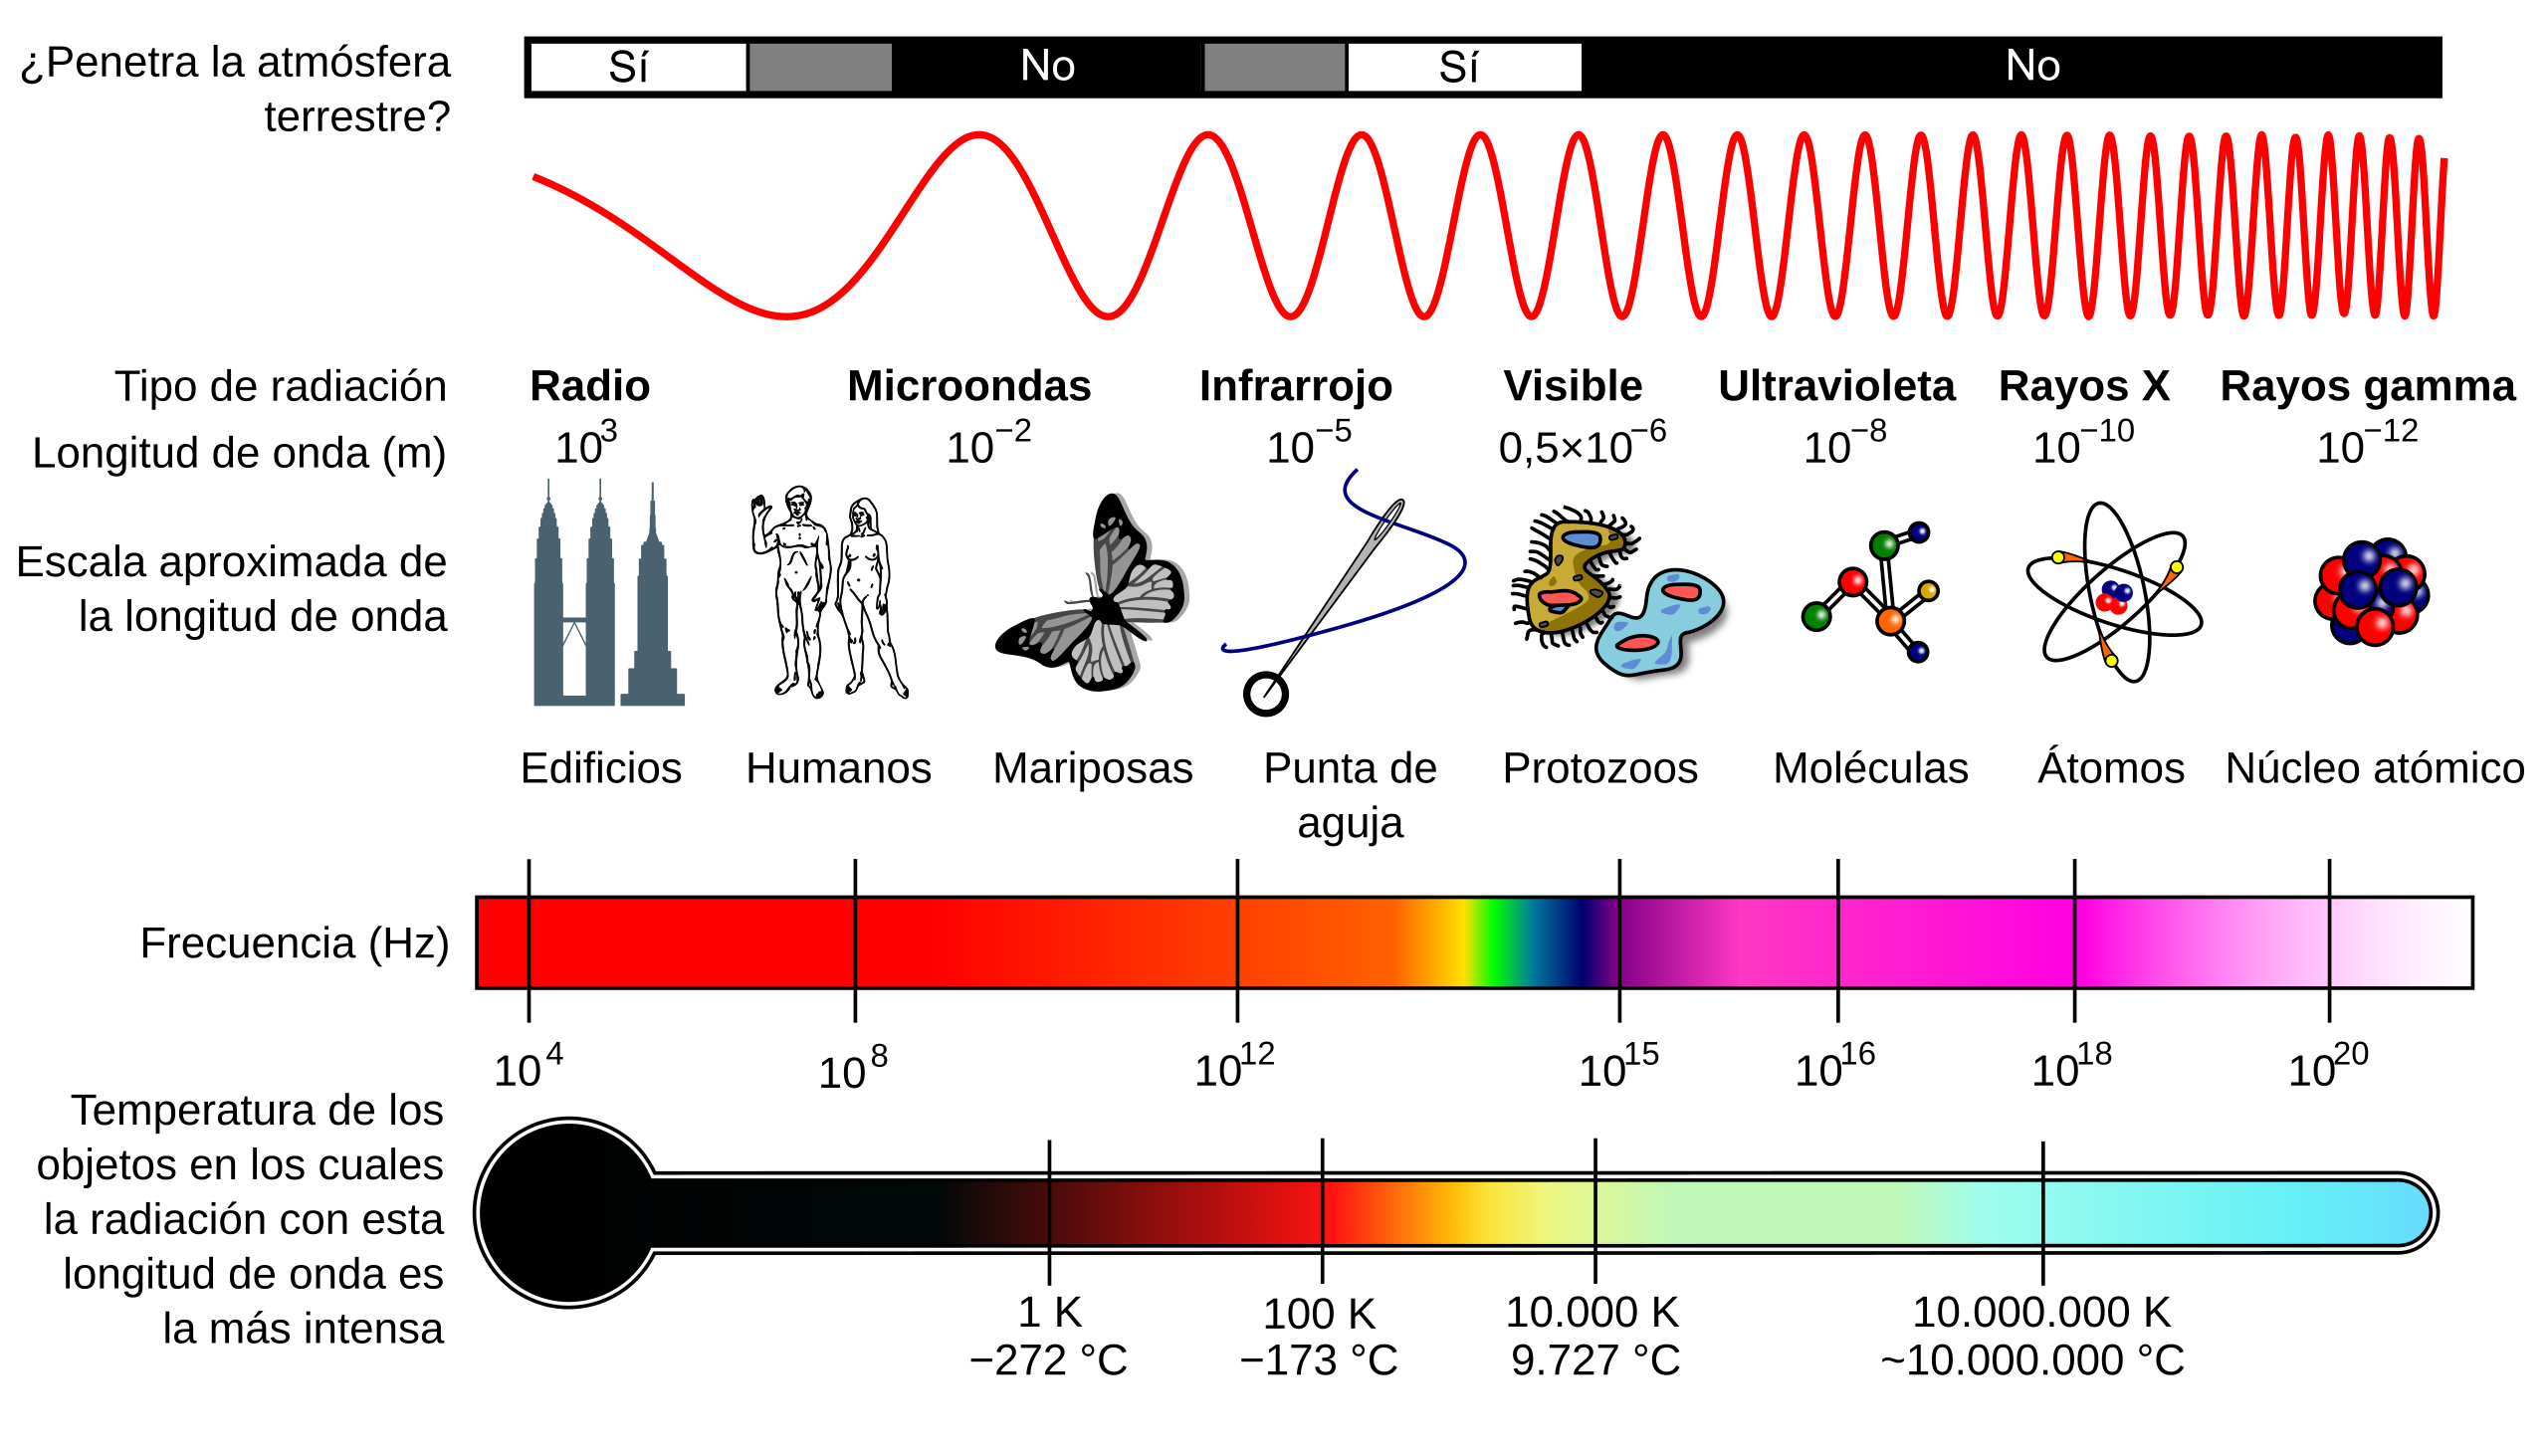
\includegraphics[width=1\linewidth]{Figuras/Fig_Hardware_espectro_electromagnetico.png}
      \caption{Espectro electromagnético}
      \label{Fig_Hardware_espectro_electromagnetico}
    \end{figure}
    	



\section{Conceptos Erróneos sobre el Hardware de Computación Cuántica.}


\textbf{Más qubits = mejor ordenador cuántico $\rightarrow$ Falso!!}
\begin{itemize}
\item La ``longitud'' del cálculo que se puede ejecutar es igualmente importante.
\item Además, la tasa de error de operación debe reducirse a medida que aumenta el tamaño del sistema; de lo contrario, el valor marginal disminuye a medida que se añaden más qubits.
\end{itemize}

\textbf{Mayor tiempo de coherencia = mejor ordenador cuántico $\rightarrow$ Falso!!}
\begin{itemize}
	\item La escala de energía es esencial para calcular el tiempo de cálculo ``efectivo''
	\item Tiempo de coherencia / tiempo de cada operación $\approx$ profundidad máxima del circuito
\end{itemize}

\textbf{Mientras el ordenador cuántico sea ``universal'', ¡servirá para algo! $\rightarrow$ Falso!!}
\begin{itemize}
\item  Hay muchos caminos para llegar a un ordenador cuántico inútil, en el sentido de que no aporte nada nuevo respecto a la computación clásica.
\end{itemize}

\textbf{Todos los cálculos que son intratables con los ordenadores clásicos son de alto valor. $\rightarrow$ Falso!!}
\begin{itemize}
\item Muchos tienen muy poco o ningún valor, así que encontrar cálculo que se pueden hacer en ordenadores cuánticos pero que son imposibles en ordenadores cuánticos no es suficiente. Tiene que poder calcularse algo útil.
\end{itemize}





\section{Algunos Roadmaps públicos}

\subsection{IBM}

IBM propone tener 200 qubits lógicos en 2029 (ver Fig. \ref{Fig_Hardware_ibm_roadmap}). Puede consultarse el roadmap \href{https://www.ibm.com/quantum/technology}{aquí}.

	\begin{figure}[H]
	\centering 
	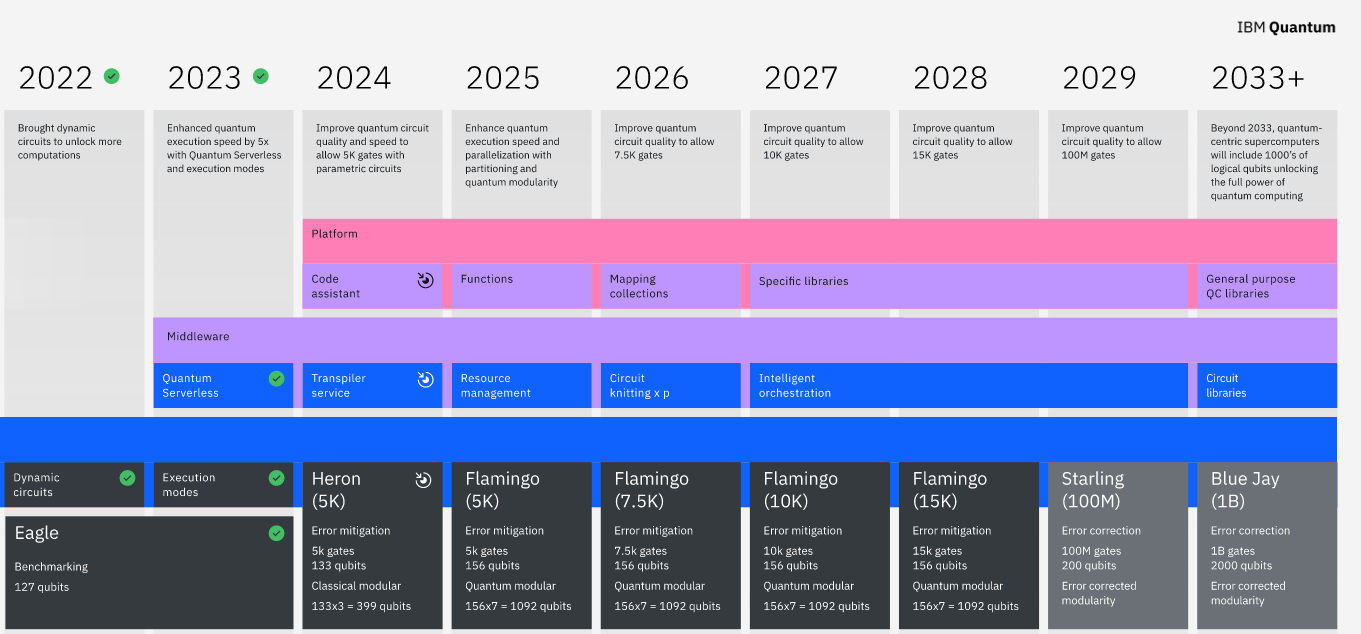
\includegraphics[width=1\linewidth]{Figuras/Fig_Hardware_ibm_roadmap.png}
	\caption{Roadmap de IBM}
	\label{Fig_Hardware_ibm_roadmap}
	\end{figure}

\subsection{Infleqtion}

Infleqtion propone tener 100 qubits lógicos en 2028 (Ver Fig. \ref{Fig_Hardware_infleqtion_roadmap}).

	\begin{figure}[H]
	\centering 
	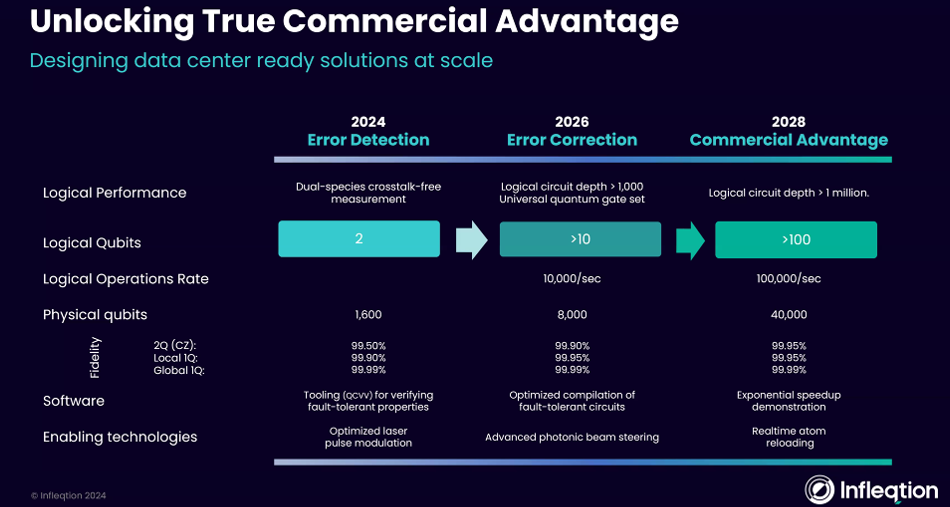
\includegraphics[width=1\linewidth]{Figuras/Fig_Hardware_infleqtion_roadmap.png}
	\caption{Roadmap de Infleqtion}
	\label{Fig_Hardware_infleqtion_roadmap}
	\end{figure}

\subsection{QuEra}

QuEra propone tener 100 qubits lógicos en 2026 (Ver Fig. \ref{Fig_Hardware_quera_roadmap})

	\begin{figure}[H]
	\centering 
	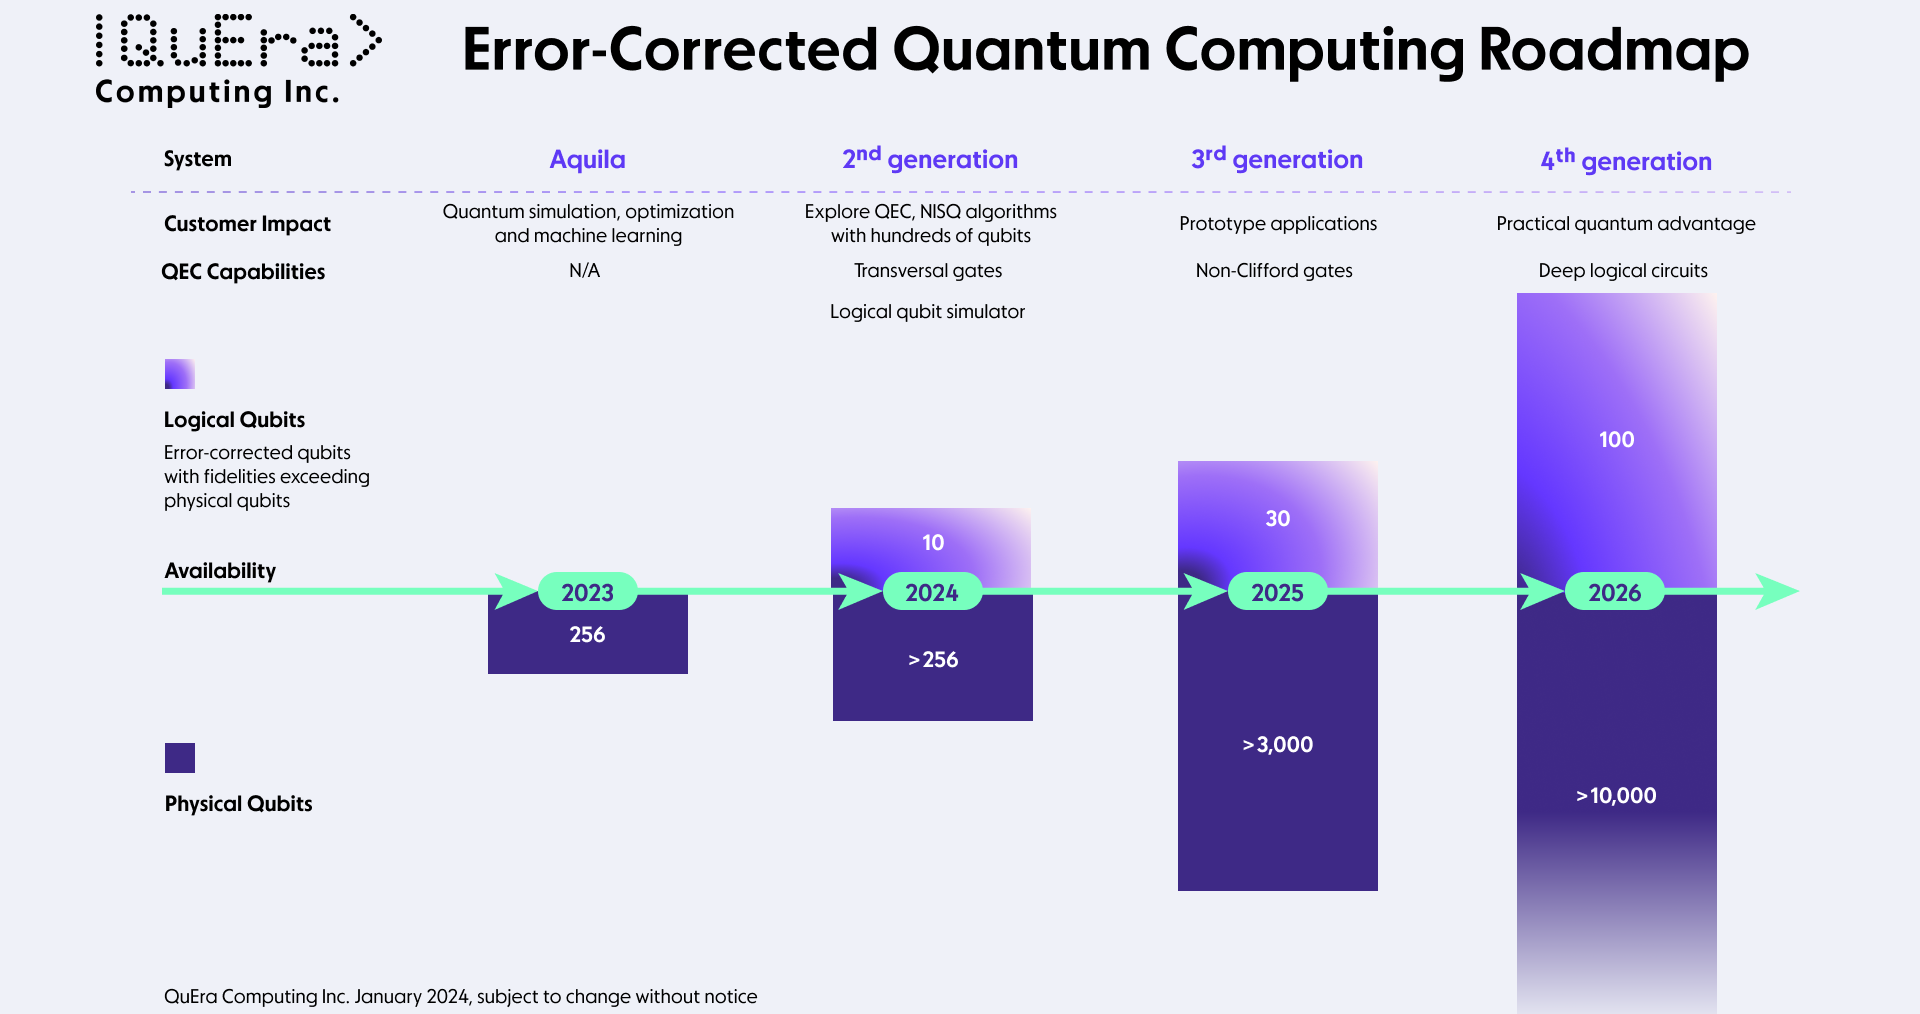
\includegraphics[width=1\linewidth]{Figuras/Fig_Hardware_quera_roadmap.png}
	\caption{Roadmap de QuEra}
	\label{Fig_Hardware_quera_roadmap}
	\end{figure}











\chapter{Computación Cuántica con Iones Atrapados (Trapped Ions)} \label{sec_chapter_hw_iones}


En este capítulo vamos a estudiar la implementación de qubit usando \textbf{iones atrapado}, viendo desde como producirlo, atraparlos y enfriarlos hasta como operar sobre ellos. Iremos viendo cuales de los Criterios de DiVicenzo de la sección \ref{sec_criterio_divicenzo} cumple está tecnología de qubits.

Este capitulo se basa en el artículo \cite{bib_ions_main}.


\section{Producción de iones.}

Antes de empezar, veamos que es un ion:

\Definicion{
Un \textbf{ion} es un núcleo o una molécula cuya nube de electrones ha sido privada (cationes) o aumentada (aniones) en una unidad, por lo que el sistema total \textit{no es eléctricamente neutrono}.
}

Entre las diversas técnicas disponibles para ionizar (positivamente) un átomo, mencionaremos brevemente la \textbf{fotoionización}. Consiste en golpear el átomo neutro con luz sintonizada a una longitud de onda adecuada, capaz de excitar un electrón externo y proporcionarle la energía suficiente para abandonar el orbital atómico. Inmediatamente después de la ionización, los iones recién creados se trasladan a un entorno protegido que retrasa la reabsorción de electrones, durante un tiempo suficiente para realizar todas las actividades experimentales requeridas.

Para las aplicaciones de computación cuántica, la elección del elemento a ionizar depende principalmente de la estructura atómica y de la energía de ionización. Elementos pertenecientes a los grupos IIA y IIB de la tabla periódica:
\begin{equation*}
\text{Be, Mg, Ca, Sr, Ba, Zn, Cd, Hg, Yb}
\end{equation*}
son los más favorables en este sentido y, por tanto, los más utilizadas.

Después de la ionización, estos elementos presentan un espectro de energía tipo Hidrógeno, con estados (\textbf{atómicos}) $\ket{a_i}$, $i \in N$, caracterizados por unos niveles de energía $E_a$, autoestados del Hamiltoniano atómico $H_a$. Dos de estos estos, que llamaremos $\ket{g}$  y $\ket{e}$ ($g$ de \textit{ground state} -estado fundamental- y $e$ de \textit{excited} -excitado-), se identificarán con los estados $\ket{0}$ y $\ket{1}$. (No exactamente, pues falta comentar los estados vibracionales).

\begin{mybox_blue}{Nota: estados atómicos y vibracionales}
Destacamos aquí que estos estados los denominamos \textbf{atómicos} para diferenciarlos de los estados \textbf{vibracionales} que veremos más adelante. 

\vspace{0.3cm}
Estos estados atómicos son los de los electrones en torno al núcleo (promociones de electrones a orbitales más externos).
\end{mybox_blue}

La transición $\ket{g} \rightarrow \ket{e}$ puede elegirse en el rango \textbf{óptico} o en el \textbf{hiperfino} seleccionando adecuadamente el estado fundamental y excitado de los orbitales iónicos. Los qubits correspondientes se denominan qubits ópticos y hiperfinos, respectivamente. Véase la Tabla \ref{Tab_ions_opticos_hiperfinos} para una comparación entre ambos. Como podemos ver, los tiempos de vida (y, por tanto, los tiempos de coherencia) de los qubits hiperfinos son mucho mayores que los qubits ópticos, lo que normalmente los convierte en la opción preferida para la computación cuántica, junto con el hecho de que también son más fáciles de manipular.

El estado actual de las técnicas de manipulación de iones permite tasas de operación de cientos de kHz, lo que significa que las operaciones básicas sobre qubits pueden realizarse en tiempos mucho menores que los tiempos de vida típicos de los qubits ópticos o de hiperfinos. Por lo tanto, los qubits ópticos y hiperfinos proporcionan una plataforma estable, bien caracterizada y rápidamente manipulable, satisfaciendo así los criterios 1a y 3 mencionados en la sección \ref{sec_criterio_divicenzo}.

\begin{table}[H]
\centering
\begin{tabular}{lll} \hline
Propiedades & Qubits opticos & Qubits hiperfinos \\ \hline
Rango & Visible, 405-790 THz & Microondas, 1-100 GHz \\
Tiempo de Vida & $\approx$ 1 s & $\approx$ 10 min \\
Estados & Nivel $S$ y un estados metaestables & Dos niveles  hiperfinos \\
Ejemplos & $6S_{1/2} \equiv \ket{g}$ y $5D_{5/2} \equiv \ket{e}$ del Ba${}^+$ & ${}^2S_{1/2} (F=1,m_F=0) = \ket{g}$ y \\
 & & ${}^2S_{1/2} (F=0,m_F=0) \equiv \ket{e}$ de Cd${}^+$ \\ \hline
\end{tabular}
\caption{Diferencias entre qubits ópticos e hiperfinos con iones.}
\label{Tab_ions_opticos_hiperfinos}
\end{table}



\section{Trampas de iones}

Un ion fotoionizado recién nacido tiene típicamente una energía de $\sim$1 keV, lo que corresponde a una velocidad de $\sim$1 m s${}^{-1}$ para un ion como el 40Ca${}^+$. A tales energías, el ion puede considerarse un sistema clásico desde el punto de vista del movimiento. Por tanto, para construir un sistema completamente cuántico necesitamos restringir su movimiento tanto en el espacio (atraparlo) como en velocidad (enfriarlo).

Una \textbf{trampa de iones} es un dispositivo cuya finalidad es mantener los iones confinados en una estrecha región del espacio. Una condición necesaria para que esto ocurra es que el ion sienta un \textbf{mínimo} de la energía potencial $V(x)$ (el centro de la trampa) en algún punto dentro de la región de atrapamiento. 

\begin{mybox_blue}{Nota: Energía potencial}
Una buena forma de explicar los mínimos de la energía potencial es usando la energía potencial gravitatoria, es decir, la generada por la fuerza de la gravedad. 
\vspace{0.3cm}

En el caso de la energía potencial gravitatoria, esta crece a medida que nos alejamos del centro de la Tierra. Es decir, una pelota en lo alto de un edificio tiene \textbf{más} energía potencial gravitatoria que a la altura de la calle. Por ese motivo, si soltamos la pelota desde lo alto, esta caerá  (hacía la zona con menos energía potencial). A medida que vaya cayendo, la pelota \textbf{perderá} energía potencial y \textbf{ganará} energía cinética (velocidad), conservándose la cantidad total de energía.
\vspace{0.3cm}

El resumen es que, cuando tenemos una fuerza central (como la gravitatoria o la eléctrica) esta trae consigo un potencial. Los objetos que sienten estas fuerzas se mueven hacia zonas de menos potencial.
\end{mybox_blue}


Aprovechando la naturaleza cargada de los iones, se puede crear un potencial de atrapamiento utilizando una combinación adecuada de potenciales eléctricos y/o magnéticos. Existen dos paradigmas para el diseño de dicho potencial de atrapamiento: 

\begin{itemize}
\item La trampa de Penning, en la que se utilizan potenciales eléctricos y magnéticos \textbf{estáticos}. 

\item La trampa de Paul, en la que se utilizan campos eléctricos \textbf{estáticos y oscilantes}.
\end{itemize}

Aunque ambos son en principio adecuados para aplicaciones de computación cuántica, la trampa de Paul es actualmente el método más utilizado en entornos académicos e industriales. 

Suficientemente cerca del centro de la trampa (del mínimo del potencial), cualquier potencial puede aproximarse bien mediante una función cuadrática de las coordenadas, es decir, un ion atrapado se comportará como un oscilador armónico simple (SHO) en tres dimensiones. 

Los sistemas de captura más utilizados en aplicaciones de computación cuántica son las \textbf{trampas lineales}: la fuerza de captura en dos de las tres dimensiones es mucho mayor que la de la tercera (por ejemplo, una trampa Paul muy fuerte en las direcciones $x$ e $y$ y un par de electrodos relativamente más débiles en la dirección $z$, como en la Fig. \ref{Fig_ions_linear_trap}), por lo que el único movimiento relevante será un \textbf{movimiento armónico simple} en (digamos) la dirección $\hat{z}$, caracterizado por una frecuencia $\omega_z$ y por la masa $M$ del ion.

	\begin{figure}[t]
	\centering 
	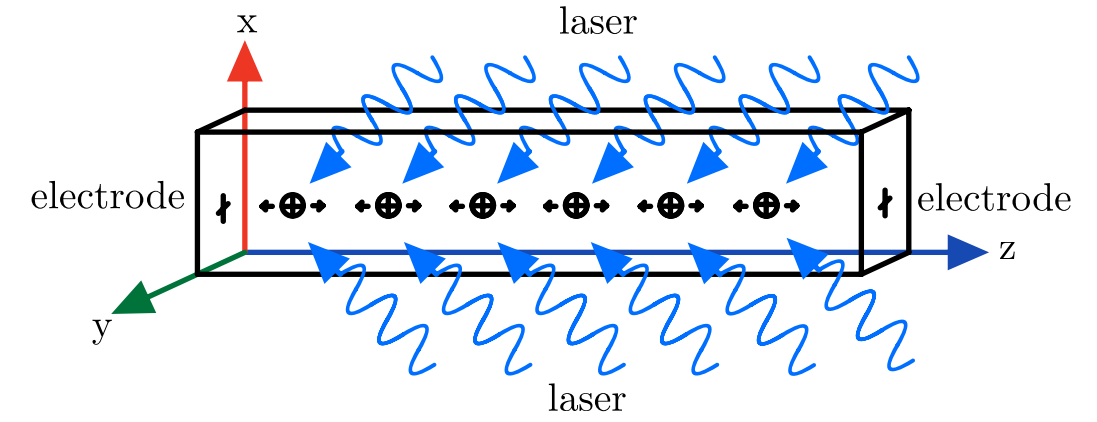
\includegraphics[width=0.6\linewidth]{Figuras/Fig_ions_linear_trap.png}
	\caption{Iones fuertemente atrapados por una trampa Paul en el plano $xy$, y a los que sólo se permite moverse en la dirección $z$. Un par de electrodos impiden que los iones se repelan fuera de la trampa. Fuente \cite{bib_ions_main}.}
	\label{Fig_ions_linear_trap}
	\end{figure}

Para que la aproximación armónica se mantenga, el ion no debe alejarse apreciablemente del centro de la trampa. Si esto ocurre, ya no podemos garantizar que las fuerzas que actúan sobre el ion se dirijan hacia el centro de la trampa, y en algún momento podríamos incluso hallarlo fuera de la trampa.

Por la razón anterior, es importante que el ion se mueva lentamente, por lo que queremos disminuir su energía cinética. Con un ligero abuso del lenguaje llamamos a esta etapa ``enfriamiento'' asociando una temperatura a la energía cinética, aunque el ion no esté en equilibrio térmico. En la sección \ref{sec_ions_laser_cooling} describiremos dos ejemplos de enfriamiento por láser, válidos en los regímenes clásico y cuántico, respectivamente. Utilizando láseres convenientemente sintonizados, es posible impartir una fuerza de amortiguación efectiva sobre los iones, que los ralentiza.

Por último, las colisiones con otras partículas también son perjudiciales para el procedimiento de atrapamiento, ya que pueden inducir cambios bruscos en la energía cinética, lo que puede provocar el escape de iones de la trampa. Para minimizar tales interacciones, se crea un \textbf{vacío ultraalto} a presiones de unos $10^{-11}$ Torr ($\sim 1,3 \times 10^{-9}$ Pa) en la región donde se colocará la trampa.



\section{Enfriamiento de iones por láser} \label{sec_ions_laser_cooling}


Como se mencionó en la sección anterior, podemos identificar dos regímenes en el enfriamiento dependiendo de cómo la energía oscilatoria media $\langle H_{SHO} \rangle$ se compara con la energía característica del oscilador armónico simple cuántico (QSHO de sus siglas en inglés), $\hbar \omega_z$:

\begin{itemize}
\item Un régimen clásico, donde el ion puede considerarse un resorte clásico, y los fenómenos cuánticos pueden despreciarse. Se trata de una buena aproximación siempre que $\langle H_{SHO} \rangle$ sea mucho mayor que $\hbar \omega_z$;

\item Un régimen cuántico, donde por el contrario $\langle H_{SHO} \rangle$ es comparable a $\hbar \omega_z$, y los efectos cuánticos adquieren importancia.
\end{itemize}

Nuestro objetivo es bajar los iones al estado fundamental del QSHO, que puede utilizarse como qubit fiduciales o $\ket{0}$ sobre el que se pueden realizar cálculos (criterio 2 de la sección 5). Esto suele ser un proceso de dos pasos: (a) enfriar el sistema hasta el punto en el que los grados de libertad (dof) vibracionales del QSHO se activan, y (b) llevar el QSHO a su estado fundamental. En las dos subsecciones siguientes se describen los métodos más utilizados para conseguirlo.


\subsection{Régimen Clásico: enfriamiento de Doppler.}


Un ion se encuentra normalmente en el régimen clásico cuando se produce. El principal método utilizado para enfriarlo hasta el régimen cuántico se conoce como enfriamiento Doppler, que utiliza el desplazamiento Doppler como método de enfriamiento subyacente. 

Como primer paso, se elige una transición resonante entre dos estados atómicos del ion con frecuencia $\omega_0$ y anchura de línea $\Gamma$, que representa la anchura de los máximos de absorción en el espacio de frecuencias. $\Gamma$ suele ser mucho mayor que la frecuencia $\omega_z$ del QSHO, de modo que los niveles QSHO quedan sin resolver. 

Estos iones se irradian con un láser monocromático con frecuencia sintonizada a un valor ligeramente inferior a la frecuencia de transición: $\omega_{abs} = \omega_0 - \delta \omega$ y vector de onda $\vec{k}$ (momento $\hbar \vec{k}$). 

Consideremos ahora la dispersión (scattering) de un ion que se mueve con velocidad $\vec{v}$ en dirección contraria a los fotones del láser. Supongamos que el ion absorbe un fotón pasa a un estado excitado y vuelve a decaer espontáneamente emitiendo un fotón en una dirección aleatoria con la misma energía. Podemos ver este proceso en la Fig. \ref{Fig_ions_dopple_cooling}.

	\begin{figure}[t]
    	\centering 
    	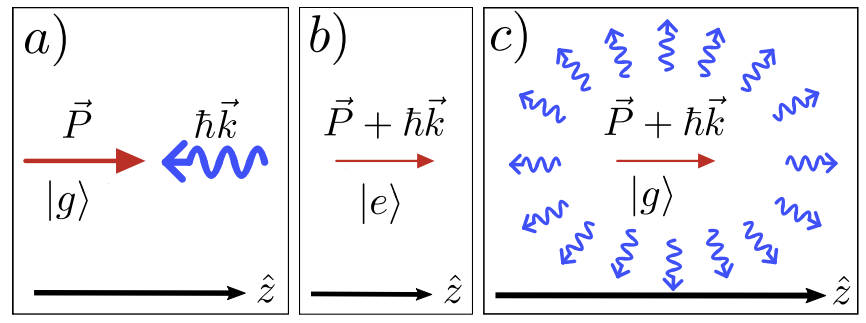
\includegraphics[width=0.8\linewidth]{Figuras/Fig_ions_dopple_cooling.png}
    	\caption{En el proceso de enfriamiento Doppler, a) y b): un ion absorbe un láser desplazado al rojo que viene hacia él y c) lo emite en una dirección aleatoria. El grosor de las flechas representa la magnitud del momento. En la figura b), debido a la absorción de un fotón que se mueve en dirección opuesta, el momento total de la partícula será menor, de ahí que la flecha sea más fina. Tras la emisión isótropa de un fotón en figure c), el momento medio de la partícula no cambia. Fuente \cite{bib_ions_main}.}
    	\label{Fig_ions_dopple_cooling}
	\end{figure}


Aplicando las ecuaciones de conservación de energía y momento, puede verse que en este proceso el fotón emitido tiene más energía que el absorbido (en concreto, $- \hbar \vec{v} \cdot \vec{k}$ más energía, donde este término es positivo pues los vectores tiene sentido contrario). 

    \begin{proof}
        Veamos este resultado. Partimos de la ecuación de conservación de energía 
        	\begin{equation} \label{ec_ions_energy}
        	\hbar \omega_{abs} + \frac{1}{2} M v^2 = \hbar \omega_0 + \frac{1}{2}M{v'}^2
        	\end{equation}
        donde a la izquierda tenemos el estado inicial y la derecha el estado final, $M$ es la masa del ión, $v$ la velocidad inicial de ión y $v'$ la velocidad de ión después de la absorción. En concreto, la que tenemos es: energía del fotón + energía cinética del ión antes de la absorción = Energía de transición (ganada por el ión al producirse la transión) + energía cinética después de la absorción.
        
        Por otro lado, tenemos la ecuación de conservación del momento:
        	\begin{equation} \label{ec_ions_momento}
        	M \vec{v} + \hbar \vec{k} = M \vec{v'}
        	\end{equation}
        
        Sustituyendo $\vec{v'}$ de la Ec. \ref{ec_ions_energy} en \ref{ec_ions_momento}, tenemos
        	\begin{equation}
        	\omega_0 = \omega_{abs} - \vec{v} \cdot \vec{k} - \frac{\hbar k^2}{2M}
        	\end{equation}
        En el lado derecho, el segundo término es el conocido \textbf{desplazamiento Doppler}, y el tercer término se conoce como \textbf{desplazamiento de retroceso}, que suele ser pequeño en comparación con el desplazamiento Doppler a altas velocidades. Despreciando el tercer término e invirtiendo la expresión, obtenemos
        	\begin{equation}
        	\omega_{abs} = \omega_0 + \vec{v} \cdot \vec{k}
        	\end{equation}
        Como $\vec{v}$ y $\vec{k}$ tiene direcciones opuestas, tenemos que $-\vec{v} \cdot \vec{k} <0$, con lo que $\omega_{abs} < \omega_0$. Es decir, cuando el fotón y el ión se mueven en sentido contrario, la energía que tiene que tener el fotón para ser absorbido es \textbf{menor}  que la energía de transición en una cantidad $\hbar \vec{v} \cdot \vec{k}$. 
        
        Por otro lado, si consideramos el proceso de emisión y hacer un tratamiento similar llegamos a:
        	\begin{equation}
        	\omega_0 = \omega_{em} - \vec{v'} \cdot \vec{k_{em}} + \frac{\hbar k_{em}^2}{2M}
        	\end{equation}
        Si nuevamente estamos a altas velocidades, podemos despreciar otra vez el desplazamiento de retroceso y quedarnos con que la frecuencia del fotón emitido es
        	\begin{equation}
        	\omega_{em} = \omega_0 + \vec{v'} \cdot \vec{k_{em}}
        	\end{equation}
        Pero en este caso el vector de onda del fotón emitido $\vec{k_{em}}$ está en una dirección aleatoria. Por lo tanto, promediando sobre un número de procesos de dispersión obtenemos $\langle \vec{v'} \cdot \vec{k_{em}} = 0 \rangle$. Entonces, en promedio el cambio de energía del fotón por evento de dispersión es
        	\begin{equation}
        	\hbar \Delta \omega = \langle \hbar (\omega_{em}-\omega_{abs} \rangle = - \hbar \vec{v} \cdot \vec{k} \, .
        	\end{equation}
        
        La ganancia de energía del fotón es igual a la perdida de energía cinética del ión ($E_k$), es decir, $\Delta E_k = \hbar \vec{v} \cdot \vec{k} < 0$. Si interpretamos temperatura $\frac{3}{2} k_B T = E_K$, esta pérdida de energía cinética provoca el enfriamiento de los iones que se desplazan hacia el láser.
    
    \end{proof}
    



Este fenómeno en fácil de entender de forma intuitiva. Al estar moviéndose el ión hacia el fotón, por efecto Doppler la energía que tiene que llevar el fotón para ser absorbido es menos (por eso decimos que los fotones tiene freciencia $\omega_{abs} =  \omega_0 - \delta \omega < \omega_0$). En concreto, $\delta \omega = - \vec{v} \cdot \vec{k}$. 

Este proceso de enfriamiento de los iones no dura indefinidamente, sino que está limitado por el desplazamiento de retroceso (\textit{recoil shift}). Es decir, este proceso funciona siempre y cuando se cumpla 
	\begin{equation}
 	-h \vec{v} \vec{k} > \hbar^2 k^2/M\,, \quad \text{con } \vec{v} \cdot \vec{k} < 0 \,.
 	\end{equation} 
Este límite para la temperatura mínima que se puede alcanzar se denomina \textbf{recoil limit}.



\subsection{Régimen Cuántico: sideband cooling}


Una vez que el enfriamiento Doppler alcanza su límite, la energía del ion es lo suficientemente baja como para considerar los grados de libertad vibracionales del QSHO. Por lo general, después del enfriamiento Doppler, el estado medio del número QSHO del ion es $ \langle n \rangle \sim 10$. Sin embargo, como se ha indicado anteriormente, nuestro objetivo es alcanzar el estado fundamental del oscilador armónico, es decir, $\ket{n}=0$, para inicializar el qubit (ver Fig. \ref{Fig_Hardware_Oscilador_Armonico}). Esto requiere un mayor enfriamiento del sistema, que generalmente se logra mediante un proceso llamado \textbf{sideband cooling}. 

Para el \textit{sideband cooling}, se elige una transición atómica con un ancho de línea $\Gamma_s$, ahora pequeño en comparación con $\omega_z$ (\textbf{frecuencia del QSHO}) para que el pico de absorción pueda distinguir las frecuencias $\omega_0 \pm \omega_z$ de $\omega_0$ (a diferencia del enfriamiento Doppler en el que $\Gamma \gg \omega_z$). Por esta razón, se elige una transición diferente a la del proceso de enfriamiento Doppler. Llamamos a los niveles inferior y superior de esta transición el estado interno fundamental $\ket{g}$ y el estado excitado $\ket{e}$, respectivamente, y denotamos esta \textbf{frecuencia de transición entre estados atómicos} como $\omega_0$. Es decir:

\begin{figure}[t]
  \centering 
  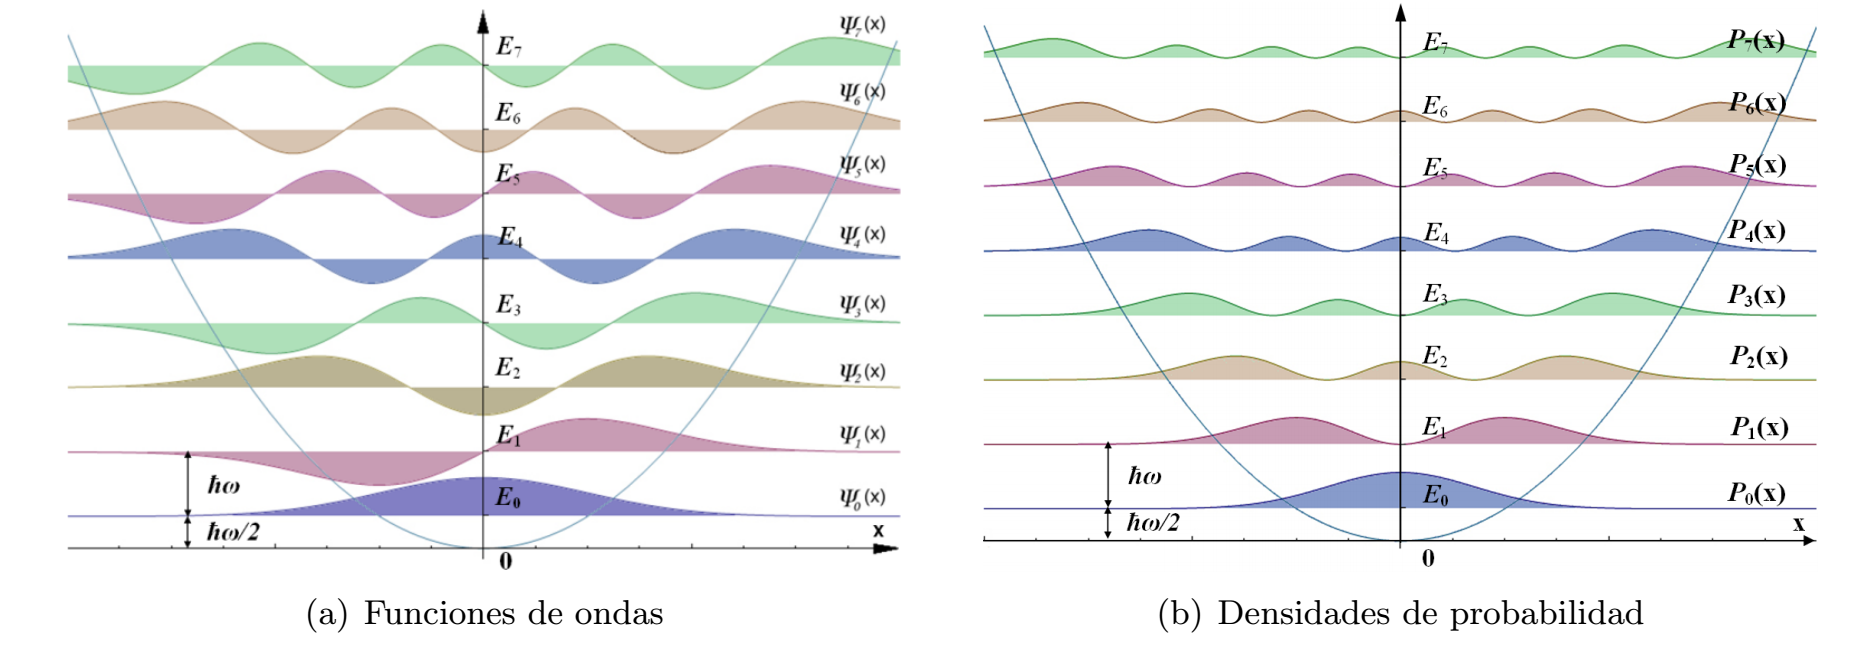
\includegraphics[width=1\linewidth]{Figuras/Fig_Hardware_Oscilador_Armonico.png}
  \caption{Primeros $8$ estados del oscilador armónico cuántico ($n=0,1, \dots,7$) en una dimensión ($\hat{x}$). El eje horizontal representa la posición $x$. Source \cite{bib_Hardware_Wiki_QHO}}
  \label{Fig_Hardware_Oscilador_Armonico}
\end{figure}

\begin{equation} 
\begin{aligned}
\omega_z & \rightarrow \text{Frecuencia del QSHO: frecuencia entre los estados } \ket{n} \\
\omega_0 & \rightarrow \text{Frecuencia de la transición atómica } \ket{g} \rightarrow \ket{e}
\end{aligned}
\end{equation}

Inicialmente, el ion se encuentra en el estado $\ket{g,n}$ con $n \sim 10$. Aquí, la notación $\ket{g,n}$ significa que el ion está en estado atómico $\ket{g}$ y en estado vibracional QSHO $\ket{n}$. Queremos alcanzar el estado básico $\ket{g,0}$ para inicializar nuestro qubit operacional. Esto se consigue mediante una repetición de las siguientes transiciones:
	\begin{equation}
	\ket{g,n} \rightarrow \ket{e,n-1} \rightarrow \ket{g, n-1} \rightarrow \{ \dots \}
	\end{equation}
	



Este conjunto de transiciones se lleva a cabo mediante la interacción de iones con un láser. En concreto, el láser induce transiciones entre el estado fundamental y el estado excitado, pero reduciendo en uno el número de ocupación del QSHO, es decir, $\ket{g,n} \rightarrow \ket{e,n-1}$. Después, las transiciones $\ket{e,n-1} \rightarrow \ket{g, n-1}$ son decaimiento espontáneos. Podemos ver este proceso en la Fig. \ref{Fig_ions_sideband_cooling}.

Para inducir la transición deseada,  $\ket{g,n} \leftrightarrow \ket{e,n-1}$, este láser se toma con una frecuencia $\omega = \omega_0 - \omega_z$. Esta elección particular de la frecuencia del láser se conoce como \textbf{red sideband resonance}.

	\begin{figure}[b]
	\centering 
	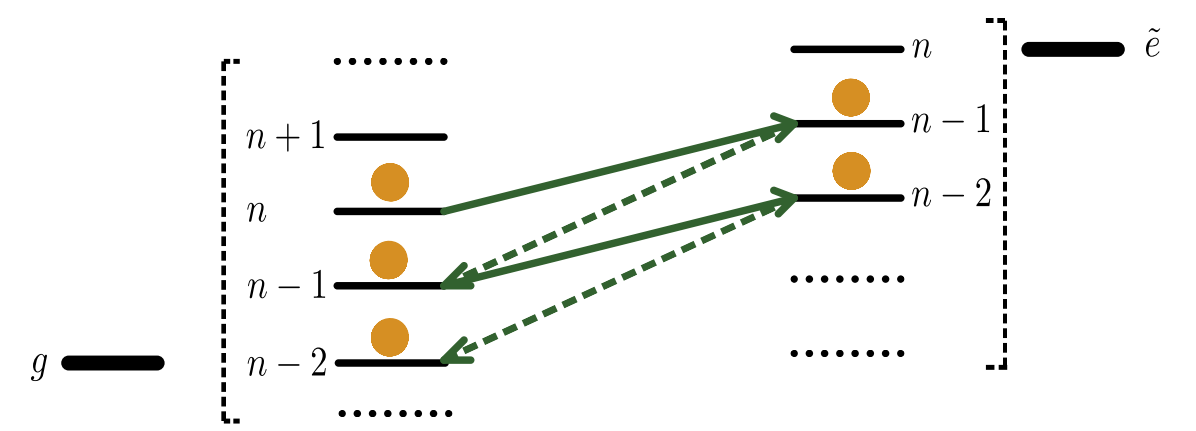
\includegraphics[width=0.7\linewidth]{Figuras/Fig_ions_sideband_cooling.png}
	\caption{La figura muestra el esquema del \textit{sideband cooling}. Las líneas continuas y discontinuas representan los procesos de absorción estimulada y emisión espontánea, respectivamente. Fuente \cite{bib_ions_main}.}
	\label{Fig_ions_sideband_cooling}
	\end{figure}



\section{Manipulando iones individuales: puertas simples} \label{sec_ions_single_ion}

\subsection{Tres tipos de resonancias}

En la sección anterior vimos que, eligiendo la frecuencia del láser, podemos utilizar la interacción láser-ión para alterar el estado del ion. En particular, mostramos que \textbf{red sideband resonance} se utiliza para una transición que reduce el estado de vibración saltando a un estado atómico excitado:
	\begin{equation}
	\boxed{\ket{g,n+1} \leftrightarrow \ket{e,n}}
	\end{equation}
(Véase que se ha hecho el cambio $n \rightarrow n+1$ respecto a la notación de la sección anterior). 
 En esta sección, introducimos dos interacciones resonantes más que se utilizan para manipular un ion durante el proceso de computación cuántica:

\begin{itemize}
\item \textbf{Blue sideband resonance}: Si tomamos como frecuencia del láser $\omega = \omega_o + \omega_z$, se puede inducir la transición
	\begin{equation}
	\boxed{\ket{g,n} \leftrightarrow \ket{e,n+1}}
	\end{equation}
	
\item \textbf{Carrier resonance}: Si la frecuencia del láser es igual a la frecuencia de transición atómica, $\omega = \omega_0$, podemos inducir la transición:
	\begin{equation}
	\boxed{\ket{g,n} \leftrightarrow \ket{e,n}}
	\end{equation}
donde no se cambia el estado de vibración.
\end{itemize} 

Una vez tenemos el estado fiducial $\ket{g,0}$ al final del proceso de enfriamiento ($n=0$), estos tres procesos de resonancia nos permiten movernos entre los 4 estados 
	\begin{equation}
	\lch \ket{g,0}, \ket{g,1}, \ket{e,0}, \ket{e,1} \rch.
	\end{equation}
Es decir, podemos tomar estos 4 estados como una base en la que expresar el estado del ión bajo la aplicación de estos tres pulsos láser:
	\begin{equation} \label{ec_ions_psi_1_ions}
	\ket{\Psi_{ion}} = \begin{pmatrix} a_{g0} \\ a_{g1} \\ a_{e0} \\ a_{e1} \end{pmatrix} = 
	a_{g0} \ket{g,0} + a_{g1} \ket{g,1} + a_{e0} \ket{e,0} + a_{e1} \ket{e,1} 
	\end{equation}
donde $|a_{g0}|^2+|a_{g1}|^2+|a_{e0}|^2+|a_{e1}|^2 = 1$.

Podemos ver los tres tipos de transiciones en la Fig. \ref{Fig_ions_Niveles_energia}.

	\begin{figure}[t]
	\centering 
	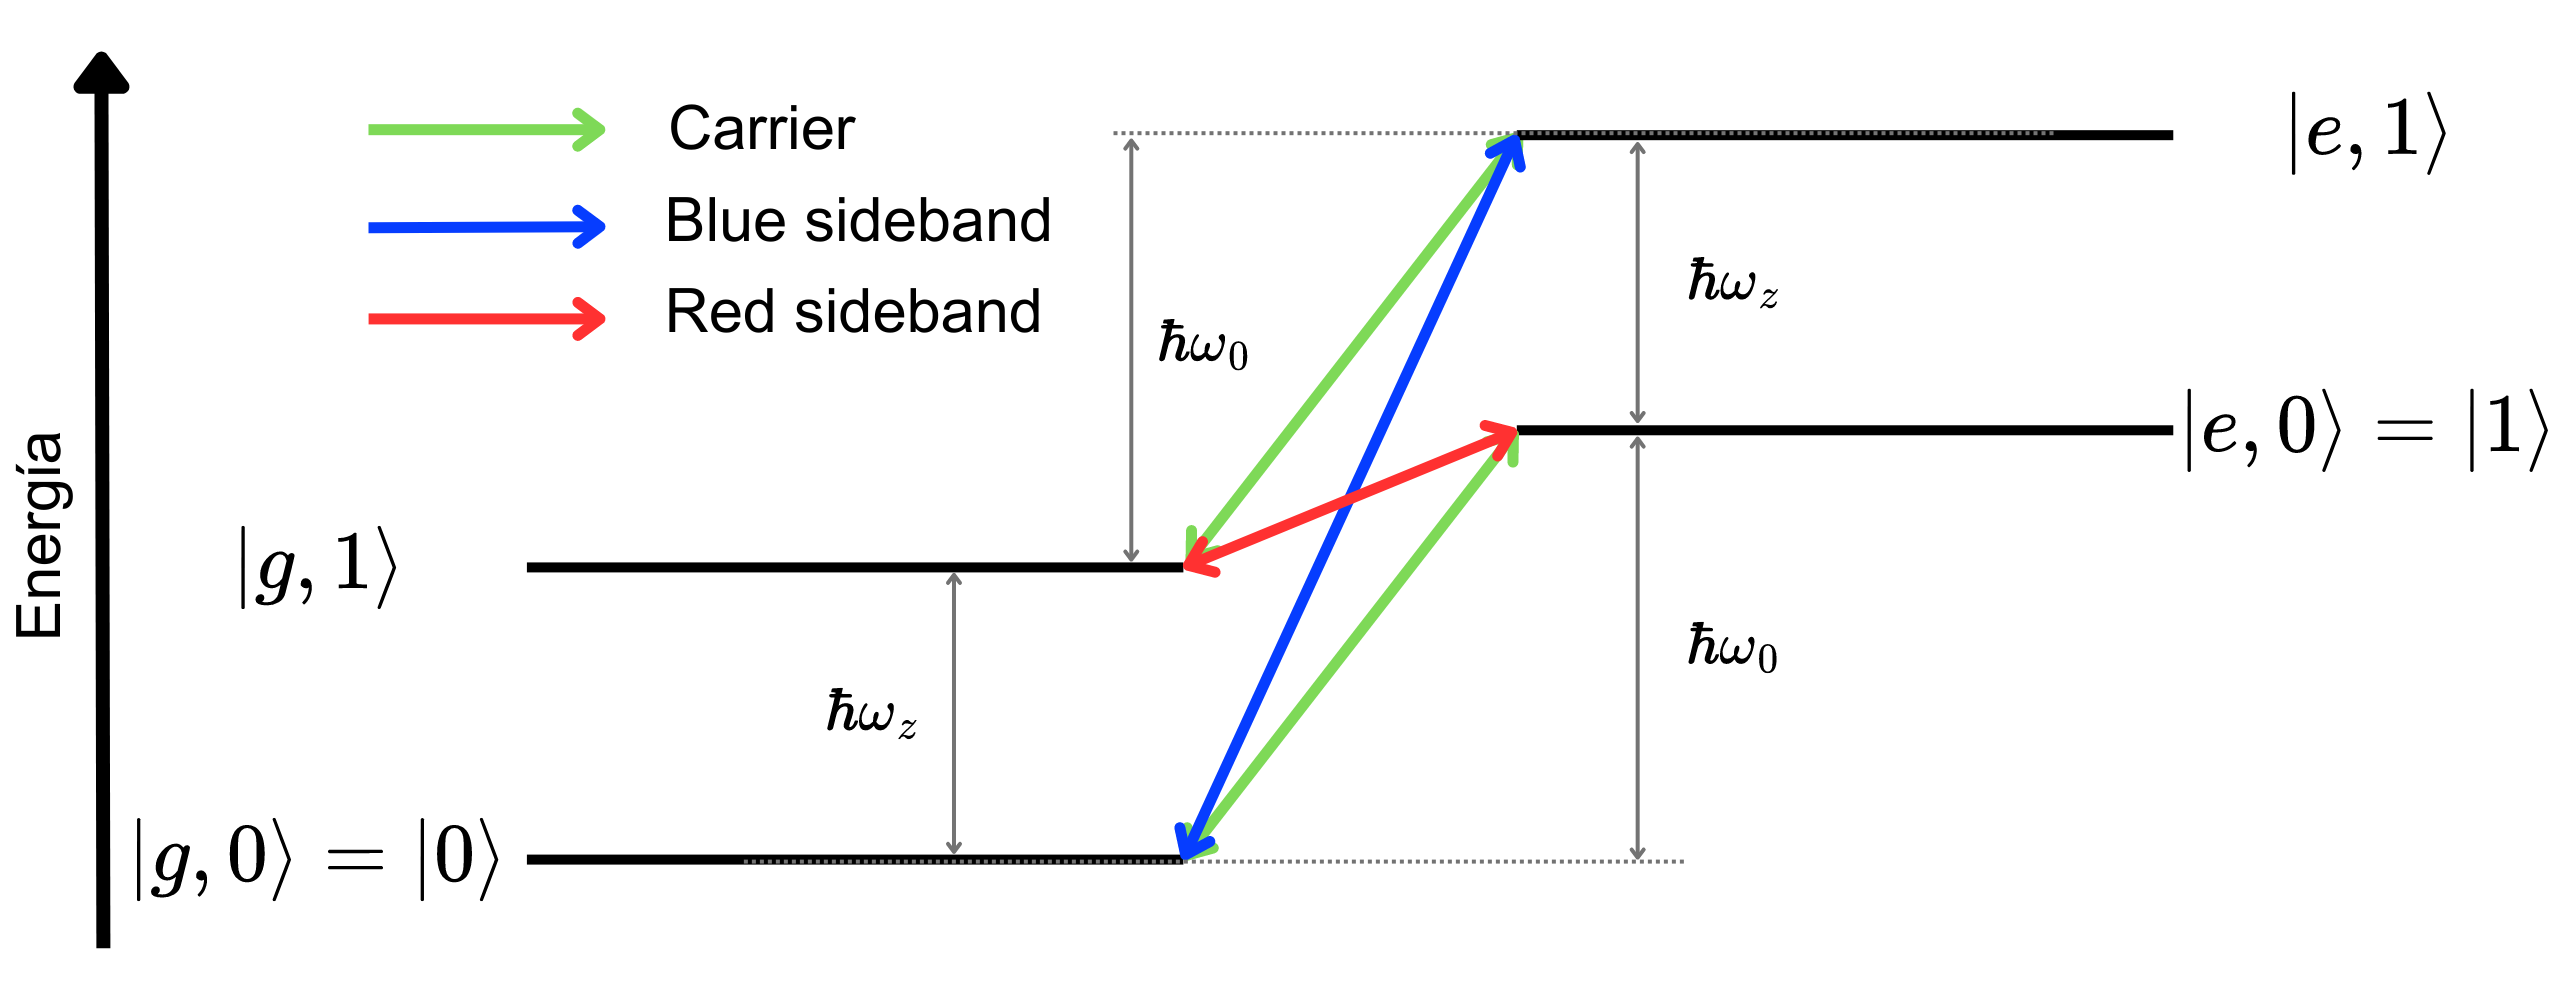
\includegraphics[width=1\linewidth]{Figuras/Fig_ions_Niveles_energia.png}
	\caption{Niveles de energía para dos estados \textbf{atómicos} $g$ y $e$ de los iones y dos estados del \textbf{oscilador armónico simple cuántico} (QSHO) $n=0$ y $n=1$.}
	\label{Fig_ions_Niveles_energia}
	\end{figure}

\subsection{Operadores de evolución temporal de las tres transiciones}

En esta sección vamos a presentar los operadores de evolución temporal de las tres transiciones que vimos en la sección. Estos operadores pueden calcularse a planteando el Hamiltoniano de interacción luz-materia \cite{bib_Haken1970}, pero está fuera del alcance de este curso. Vamos simplemente a poner el resultado.

		\SubsubiIt{Carrier resonance}


% \makebox[\widthof{$\ket{g,n}$}]{$0$}
% \makebox[\widthof{$\ket{g,n+1}$}]{$0$}  
% \makebox[\widthof{$\ket{e,n}$}]{$0$}
% \makebox[\widthof{$\ket{e,n+1}$}]{$0$}
Para este caso tenemos 
%\begin{equation} \label{ec_ions_U_carrier}
% \begin{matrix}
%    & 
    %
%    \begin{matrix}
%      \makebox[\widthof{$-i e^{i \phi} \sin \lp \beta/2 \rp$}]{$\ket{g,n}$}   & 
%      \ket{g,n+1} & 
%      \makebox[\widthof{$-i e^{-i \phi} \sin \lp \beta/2 \rp$}]{$\ket{e,n}$}   &
%      \ket{e,n+1}
%    \end{matrix} 	&  \\[.5\normalbaselineskip]
  %
%    \mathcal{U}_I^{(\text{c})} = & 
%    \begin{bmatrix}
%        \cos \lp \beta/2 \rp  & 
%        \makebox[\widthof{$\ket{g,n+1}$}]{$0$}   & 
%        -i e^{-i \phi} \sin \lp \beta/2 \rp & 
%        \makebox[\widthof{$\ket{e,n+1}$}]{$0$} \\
      %
%        0   & 
%        \makebox[\widthof{$\ket{g,n+1}$}]{$1$}   & 
%        0 & 
%        \makebox[\widthof{$\ket{e,n+1}$}]{$0$} \\
      %
%        -i e^{i \phi} \sin \lp \beta/2 \rp & 
%        \makebox[\widthof{$\ket{g,n+1}$}]{$0$}   & 
%        \cos \lp \beta/2 \rp & 
%        \makebox[\widthof{$\ket{e,n+1}$}]{$0$} \\
      %
%        0 & 
%        \makebox[\widthof{$\ket{g,n+1}$}]{$0$}   & 
%        0 & 
%        \makebox[\widthof{$\ket{e,n+1}$}]{$1$} 
%    \end{bmatrix} &
%    \begin{matrix} \ket{g,n} \\ \ket{g,n+1} \\ \ket{e,n} \\ \ket{e,n+1} \end{matrix} 
%\end{matrix} \,
%\end{equation}

\begin{figure}[H]
    \centering 
    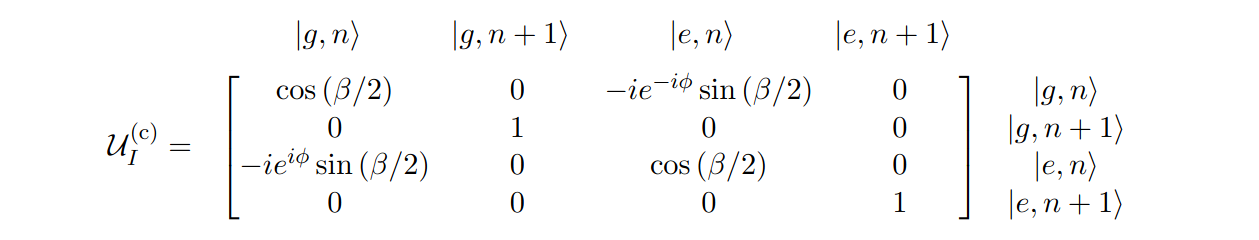
\includegraphics[width=1\linewidth]{Figuras/Fig_ions_U_carrier.png}
    \caption{Carrier resonance}
    \label{Fig_ions_U_carrier}
\end{figure}
donde $\phi$ es la \textbf{fase} del pulso láser y $\beta = \Omega t$, siendo $\Omega$ la intensidad de acoplamiento (un parámetro) y $t$ el \textbf{tiempo} de aplicación del pulso láser. Para nuestro caso, $n = 0$. 


		\SubsubiIt{Blue sideband}
		
Para este caso tenemos 
%\begin{equation} \label{ec_ions_U_bsb}
% \begin{matrix}
%    & 
%    %
%    \begin{matrix}
%      \makebox[\widthof{$-i e^{i (\phi + \pi/2)} \sin \lp \eta\beta/2 \rp$}]{$\ket{g,n}$}   & 
%      \ket{g,n+1} & 
%      \ket{e,n}   &
%      \makebox[\widthof{$-i e^{-i (\phi+ \pi/2)} \sin \lp \eta\beta/2 \rp$}]{$\ket{e,n+1}$} 
%    \end{matrix} 	&  \\[.5\normalbaselineskip]
  %
%    \mathcal{U}_I^{(\text{bsb})} = & 
%    \begin{bmatrix}
%        \cos \lp \eta\beta/2 \rp  & 
%        \makebox[\widthof{$\ket{g,n+1}$}]{$0$}   & 
%        \makebox[\widthof{$\ket{e,n}$}]{$0$}  & 
%        -i e^{-i (\phi+ \pi/2)} \sin \lp \eta\beta/2 \rp    \\
%      %
%        0   & 
%        \makebox[\widthof{$\ket{g,n+1}$}]{$1$}   & 
%        0 & 
%        0 \\
%      %
%        0 & 
%        \makebox[\widthof{$\ket{g,n+1}$}]{$0$}   & 
%        \makebox[\widthof{$\ket{e,n}$}]{$1$} & 
%        0 \\
%      %
%        -i e^{i (\phi+ \pi/2)} \sin \lp \eta\beta/2 \rp  & 
%        \makebox[\widthof{$\ket{g,n+1}$}]{$0$}   & 
%        \makebox[\widthof{$\ket{e,n}$}]{$0$} & 
%        \cos \lp \eta\beta/2 \rp  
%    \end{bmatrix} &
%    \begin{matrix} \ket{g,n} \\ \ket{g,n+1} \\ \ket{e,n} \\ \ket{e,n+1} \end{matrix} 
%\end{matrix}
%\end{equation}
\begin{figure}[H]
    \centering 
    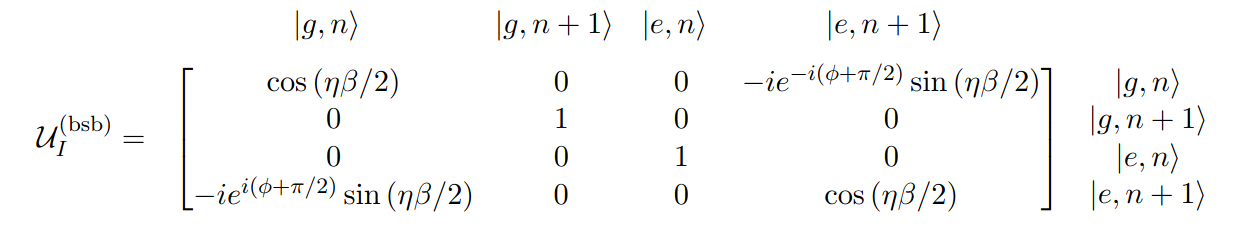
\includegraphics[width=1\linewidth]{Figuras/Fig_ions_U_bsb.png}
    \caption{Blue sideband}
    \label{Fig_ions_U_bsb}
\end{figure}
donde $\phi$ es la \textbf{fase} del pulso láser, $\eta$ el parametro de Lamd-Dicke y $\beta = \Omega t$, siendo $\Omega$ la intensidad de acoplamiento (un parámetro) y $t$ el \textbf{tiempo} de aplicación del pulso láser. Para nuestro caso, $n = 0$.

		\SubsubiIt{Red sideband}

Para este caso tenemos 
%\begin{equation} \label{ec_ions_U_rsb}
% \begin{matrix}
%    & 
%    %
%    \begin{matrix}
%      \ket{g,n}  & 
%      \makebox[\widthof{$-i e^{i (\phi+ \pi/2)} \sin \lp \eta\beta/2 \rp$}]{$\ket{g,n+1}$}  & 
%      \makebox[\widthof{$-i e^{-i (\phi+ \pi/2)} \sin \lp \eta\beta/2 \rp$}]{$\ket{e,n}$}   &
%      \ket{e,n+1}
%    \end{matrix} 	&  \\[.5\normalbaselineskip]
%  %
%    \mathcal{U}_I^{(\text{rsb})} = & 
%    \begin{bmatrix}
%        \makebox[\widthof{$\ket{g,n}$}]{$1$}  & 
%        0 & 
%        0 & 
%        \makebox[\widthof{$\ket{e,n+1}$}]{$0$} \\
%      %
%        \makebox[\widthof{$\ket{g,n}$}]{$0$}   & 
%        \cos \lp \eta\beta/2 \rp    & 
%        -i e^{-i (\phi+ \pi/2)} \sin \lp \eta\beta/2 \rp & 
%        \makebox[\widthof{$\ket{e,n+1}$}]{$0$} \\
%      %
%        \makebox[\widthof{$\ket{g,n}$}]{$0$} & 
%        -i e^{i (\phi+ \pi/2)} \sin \lp \eta\beta/2 \rp   & 
%        \cos \lp \eta\beta/2 \rp & 
%        \makebox[\widthof{$\ket{e,n+1}$}]{$0$} \\
%      %
%        \makebox[\widthof{$\ket{g,n}$}]{$0$} & 
%        0 & 
%        0 & 
%        \makebox[\widthof{$\ket{e,n+1}$}]{$1$} 
%    \end{bmatrix} &
%    \begin{matrix} \ket{g,n} \\ \ket{g,n+1} \\ \ket{e,n} \\ \ket{e,n+1} \end{matrix} 
%\end{matrix}
%\end{equation}
\begin{figure}[H]
    \centering 
    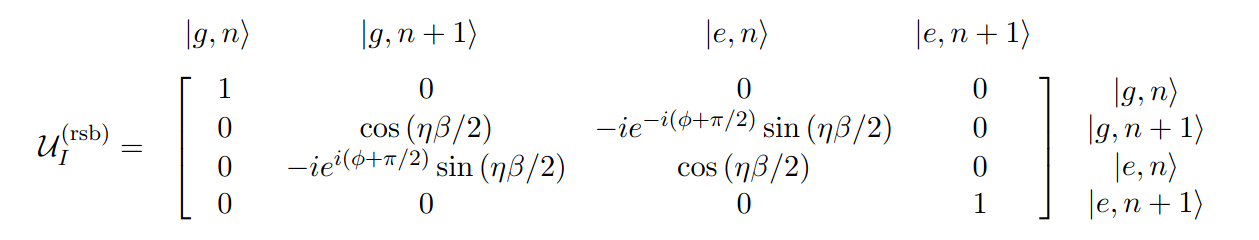
\includegraphics[width=1\linewidth]{Figuras/Fig_ions_U_rsb.png}
    \caption{Red sideband}
    \label{Fig_ions_U_rsb}
\end{figure}
donde $\phi$ es la \textbf{fase} del pulso láser, $\eta$ el parametro de Lamd-Dicke y $\beta = \Omega t$, siendo $\Omega$ la intensidad de acoplamiento (un parámetro) y $t$ el \textbf{tiempo} de aplicación del pulso láser. Para nuestro caso, $n = 0$. 



\begin{mybox_blue}{Nota}
Viendo estas matrices y como se aplican sobre los estados, vemos por qué en las transiciones estuvimos poniendo $\leftrightarrow$ en vez de $\rightarrow$. Esto es porque dependiendo del tiempo $t$ de aplicación del láser, podemos movernos entre los dos estados.
\end{mybox_blue}

\begin{mybox_blue}{Nota: Subíndice $I$}
El subíndice $I$ en los operadores de evolución temporal hace referencia a que están en la imagen de interacción. Nuevamente, esto está fuera del alcance del curso y se comenta por completitud.
\end{mybox_blue}


\subsection{Estados del Qubit y Puertas Simples con Iones}

Veamos que sucede si aplicamos el operador de evolución temporal de la \textit{carrier resonance} de la Fig. \ref{Fig_ions_U_carrier} sobre el estado $\ket{g,0}$:

	\begin{equation}
	\mathcal{U}_I^{(\text{c})} \ket{g,0} = \cos(\beta/2) \ket{g,0} - i e^{i \phi} \sin (\beta/2) \ket{e,0}\, .
	\end{equation}

Si hacemos el siguiente cambio de notación
	\begin{equation}
	\boxed{\ket{g,0} \equiv \ket{0}} \,, \quad \text{y} \quad \boxed{\ket{e,0} \equiv \ket{1}}
	\end{equation}
y tomamos $t=\theta/\Omega$ y $\phi = \varphi - \pi/2$, nos queda
	\begin{equation}
	\boxed{\mathcal{U}_I^{(\text{c})} \ket{0} = \cos(\theta/2) \ket{0} + e^{i \varphi} \sin (\theta/2) \ket{1}}\, ,
	\end{equation}
que si nos fijamos es la ecuación del \textbf{estado general de un qubit} (Ec. \ref{ec_qubit_caso_general}). Es decir, el estado general de un qubit puede considerarse el resultado de la aplicación de una puerta de un qubit al qubit fiduciario $\ket{g,0} \equiv \ket{0}$, lo que implica que puede aplicarse cualquier puerta de un qubit al qubit fiduciario utilizando la interacción de \textit{carrier resonance} y seleccionando un intervalo de tiempo y una fase adecuados para el pulso láser.

Con esto, se cumple el criterio 2 de Divicenzo (sección \ref{sec_criterio_divicenzo}).

\section{Manipulación de múltiples iones.}


Cuando hay más de un ion en la trampa, hay que tener en cuenta un fenómeno adicional. Las cargas eléctricas del mismo signo se repelen entre sí; por lo tanto, el potencial de atrapamiento y el potencial de Coulomb repulsivo entre iones competirán para determinar la densidad de iones. Como suele ocurrir cuando existe tal competencia, es posible demostrar que existe un estado de equilibrio. De hecho, para las trampas lineales a las temperaturas de trabajo habituales en los experimentos de computación cuántica, los iones tienden a formar estructuras coherentes en forma de cadena denominadas \textbf{cristales de Coulomb}. 

Una descripción completa de los modos normales y de los niveles de energía detallados que surgen del estudio de esta estructura queda fuera del alcance de este curso. Resumimos los resultados mencionando que, entre todos sus posibles comportamientos colectivos, el cristal de Coulomb exhibe el modo de centro de masa de menor energía, similar al movimiento de un único ion, pero que ahora implica a toda la cadena de partículas atrapadas moviéndose al unísono.

En al sección \ref{sec_ions_single_ion} hemos explotado la interacción entre los grados de libertad vibratorios y atómico de un único ion. Los iones de este cristal pueden seguir considerándose qubits atómicos individuales, pero desde el punto de vista del movimiento deben considerarse como una red. En consecuencia, \textbf{ya no pueden cambiar de estado vibratorios individualmente}, y las únicas transiciones energéticas permitidas serán necesariamente las asociadas a los \textbf{modos normales de la red} cuantizada correspondiente. 

Esto tiene las dos consecuencias siguientes.
\begin{itemize}
\item El estado de una cadena de $N$ iones debe describirse como el producto tensorial de $N$ qubits atómicos individuales y \textbf{un solo estado vibratorio global}:
	\begin{equation}
	\ket{x_{n-1},\nu_{n-1}}, \dots, \ket{x_0, \nu_0} \, \rightarrow \, \ket{x_{n-1} \dots x_0, \nu}  \,, \qquad \lp x_j \in \lch g,e \rch, \, \nu \in \lch n=0,n=1 \rch \rp
	\end{equation}

\item Las transiciones de \textit{red} y \textit{blue sideband} cambiarán ahora el estado vibratorio de \textbf{toda la cadena}, aunque siguen operando sobre estados atómicos \textbf{individuales} de los iones. Por ejemplo, la \textit{red sideband} aplicada al segundo ion de una cadena de dos iones da como resultado
	\begin{equation}
	\mathcal{U}_I^{\text{(rsb)}}(t) \ket{g_2, g_1, \mathbf{1}} = \cos(\nu\beta/2) \ket{g_2, g_1, \mathbf{1}} - i e^{i (\phi+\pi/2)} \sin(\nu\beta/2) \ket{e_2, g_1, \mathbf{0}} \, .
	\end{equation}

Ahora la energía intercambiada en una transición vibratoria de la red es ahora $N$ veces mayor que la implicada anteriormente en las transiciones de un solo ion, ya que $N$ iones tienen que cambiar su movimiento a la vez.
\end{itemize}

El hecho de que toda la red se vea ahora afectada por una transición vibratoria implica una especie de \textbf{interacción de largo alcance} entre los iones del cristal. Esto allana el camino para la implementación de las puertas multiqubit (la puerta CNOT) en la sección \ref{sec_ions_multiqubit}.

Las trampas lineales actuales pueden albergar aproximadamente $\sim 10^2$ iones, pero actualmente se están desarrollando propuestas para escalar el sistema (para satisfacer el criterio 1b de la sección \ref{sec_criterio_divicenzo}) mediante la construcción de redes de trampas. En estos sistemas, los fotones se utilizan para transferir información entre trampas y, más recientemente, para transportar iones.



\section{Lectura del estado de los iones}

Una vez preparado un qubit, el criterio 5 de la sección \ref{sec_criterio_divicenzo} requiere la capacidad de leer de forma fiable su estado. Sabemos que no podemos tener una descripción exhaustiva de un sistema cuántico, ya que una medición lo colapsará inevitablemente a un estado propio del observable. Por tanto, sólo podemos adoptar un enfoque probabilístico. 

Una forma estándar de sondear iones implica la selección de un estado excitado auxiliar $\ket{e'}$, que es distinto tanto del estado fundamental $\ket{g}$ como del estado excitado $\ket{e}$ dentro de la resolución de frecuencia de los instrumentos. Además, dicho estado debe ser de corta duración, es decir, decaer rápidamente de nuevo al estado fundamental $\ket{g}$.

El procedimiento de lectura es el siguiente. Dirigimos un láser sintonizado con la transición $\ket{g} \rightarrow \ket{e'}$ sobre un ion. Absorberá fotones (y los emitirá rápidamente) si el qubit del ion tiene un componente en el estado fundamental. Esta radiación puede ser detectada por fotodetectores (\textbf{estado brillante}). En cambio, un ion en estado excitado será transparente a la radiación (\textbf{estado oscuro}) y los fotodetectores no detectarán ninguna radiación. La Fig. \ref{Fig_ions_readout} resume estos conceptos. 

	\begin{figure}[h]
	\centering 
	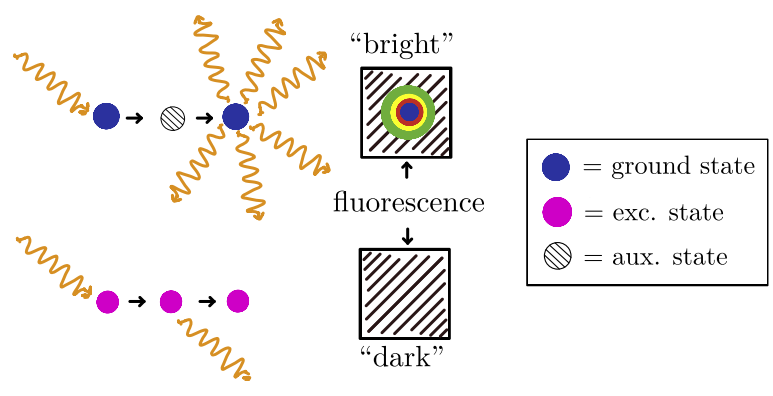
\includegraphics[width=0.7\linewidth]{Figuras/Fig_ions_readout.png}
	\caption{Los iones que interaccionan con el láser emiten fluorescencia (si están en estado fundamental) o permanecen inertes (si están en estado excitado). La radiación emitida es recogida por el fotodetector y dará lugar a un punto brillante en la superficie del detector. Fuente \cite{bib_ions_main}}
	\label{Fig_ions_readout}
	\end{figure}

Dirigir el láser a un ion equivale a medir su estado. Así, podemos expresar el proceso como el colapso de un estado objetivo
	\begin{equation}
	\ket{\Psi} = \alpha_{\text{brillo}} \ket{g} + \alpha_{\text{oscuro}} \ket{e}
	\end{equation}
al estado fundamental o al excitado, con probabilidades $P_{\text{brillo}} = |\alpha_{\text{brillo}}|^2$ y $P_{\text{oscuro}} = |\alpha_{\text{oscuro}}|^2$. Para estimar $P_{\text{brillo}}$ y $P_{\text{ocuro}}$, la preparación y la medición del estado deben repetirse un número suficientemente grande de veces. Las técnicas mencionadas pueden alcanzar una precisión del 99,99\% y superior.


\section{Puertas multiqubit con iones} \label{sec_ions_multiqubit}

Hemos demostrado que se puede preparar con precisión un sistema de iones atrapados en un estado fiduciario. Se ha demostrado experimentalmente que un sistema de este tipo es escalable hasta unos cien iones, puede manipularse utilizando la interacción láser-ión y el estado final puede leerse de forma efectiva. También hemos demostrado que se puede aplicar cualquier puerta de 1 qubit al estado inicial utilizando un pulso láser con una fase, duración y frecuencia concreta usando la \textit{carrier resonance}. 

Sin embargo, queda por ver si se puede aplicar alguna puerta de múltiples qubits al sistema. Como ya se discutió, cualquier puerta de múltiples qubits puede obtenerse utilizando puertas de 1 qubit y la puerta CNOT de 2 qubits. En esta sección, discutiremos el proceso de implementación de la puerta CNOT. Demostraremos que una puerta CNOT puede construirse utilizando puertas Hadamard y Z controladas.

Al igual que antes, definimos $\ket{g,0} \equiv \ket{0}$ y $\ket{e,0} \equiv \ket{1}$ como la base computacional.  Aunque tanto el estado atómico como los estados vibracionales pueden utilizarse como qubits separados, normalmente los qubits vibracionales sólo se consideran qubits auxiliares (para cálculo intermedio) y no como qubits medibles porque son difíciles para medir.

\subsection{Puerta de Hadammard}

La puerta de Hadammard (ver Ec. (\ref{ec_puertas_simples_H})) puede construirse (salvo una fase global) aplicando dos veces la \textit{carrier transition} (Fig. \ref{Fig_ions_U_carrier})
	\begin{equation}  \label{ec_ions_H}
	H = \mathcal{U}_I^{(\text{c})}(\beta = \pi, \phi = \pi) \mathcal{U}_I^{(\text{c})}(\beta = \pi/2, \phi = -\pi/2) \, .
	\end{equation}

\Ejercicio{
Demuestra el resultado de la Ec. (\ref{ec_ions_H}). Para ello, recuerda como la \textit{carrier transition} solo afecta a los estados  $\ket{g,0} \equiv \ket{0}$ y $\ket{e,0} \equiv \ket{1}$, la matriz $4\times4$ de la Fig. (\ref{Fig_ions_U_carrier}) puede escribirse como una matriz $2\times2$ tomando como base $\{\ket{g,0},\ket{e,0}\}$.
}



\subsection{Puerta controlada $Z$}

La puerta controlada-Z (CZ) es una puerta de dos qubits. Su acción puede describirse como:
\begin{itemize}
\item No hace nada al qubit objetivo si el qubit de control es $\ket{0}$
\item Aplica una puerta $Z$ en el qubit objetivo si el qubit de control es $\ket{1}$.
\end{itemize}
 
Como CZ es una puerta de dos qubits, necesitamos dos etiquetas para los grados de libertad atómicos de los dos iones. La base del espacio de Hilbert de dos qubits es ahora 
	\begin{equation*}
	\{\ket{gg}, \ket{ge}, \ket{eg}, \ket{ee} \}\, , 
	\end{equation*}
(todos con $n=0$) donde la primera etiqueta indica el \textbf{qubit de control} y la segunda etiqueta indica el \textbf{qubit de objetivo}. En notación matricial, la puerta CZ puede expresarse como

%\begin{equation} \label{ec_ions_CZ}
% \begin{matrix}
%    & 
    %
%    \begin{matrix}
%      \ket{gg} & 
%      \ket{ge} & 
%      \ket{eg} &
%      \ket{ee}
%    \end{matrix} 	&  \\[.5\normalbaselineskip]
  %
%    \text{CZ} = & 
%    \begin{bmatrix}
%        \makebox[\widthof{$\ket{gg}$}]{$1$} & 
%        \makebox[\widthof{$\ket{gg}$}]{$0$} & 
%        \makebox[\widthof{$\ket{gg}$}]{$0$} & 
%        \makebox[\widthof{$\ket{gg}$}]{$0$} \\
      %
%        \makebox[\widthof{$\ket{gg}$}]{$0$} & 
%        \makebox[\widthof{$\ket{gg}$}]{$1$} & 
%        \makebox[\widthof{$\ket{gg}$}]{$0$} & 
%        \makebox[\widthof{$\ket{gg}$}]{$0$} \\
      %
%        \makebox[\widthof{$\ket{gg}$}]{$0$} & 
%        \makebox[\widthof{$\ket{gg}$}]{$0$} & 
%        \makebox[\widthof{$\ket{gg}$}]{$1$} & 
%        \makebox[\widthof{$\ket{gg}$}]{$0$} \\
      %
%        \makebox[\widthof{$\ket{gg}$}]{$0$} & 
%        \makebox[\widthof{$\ket{gg}$}]{$0$} & 
%        \makebox[\widthof{$\ket{gg}$}]{$0$} & 
%        \makebox[\widthof{$\ket{gg}$}]{$-1$} \\
%    \end{bmatrix} &
%    \begin{matrix} \ket{gg} \\ \ket{ge} \\ \ket{eg} \\ \ket{ee} \end{matrix} 
%\end{matrix} \,
%\end{equation}
\begin{figure}[h]
    \centering 
    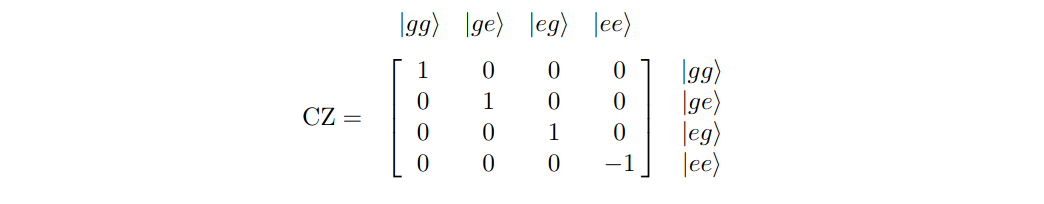
\includegraphics[width=1\linewidth]{Figuras/Fig_ions_CZ_matrix.png}
    \caption{Puerta CZ}
    \label{Fig_ions_CZ_matrix}
\end{figure}


Para implementar la puerta CZ necesitamos construir otras dos puertas de un ión que se describen a continuación.

		\SubsubiIt{Puerta de SWAP entre estados atómicos y vibracionales ($\text{SWAP}_{av}$)}

En este caso, consideramos tanto el estado atómico como el vibracional de un ion. La base de este espacio es 
	\begin{equation}
 	\lch \ket{g,0}, \ket{g,1}, \ket{e,0}, \ket{e,1} \rch.
 	\end{equation} 
La acción de la puerta $\text{SWAP}_{av}$ se representa mediante la matriz
%\begin{equation} \label{ec_ions_SWAPav}
% \begin{matrix}
%    & 
    %
%    \begin{matrix}
%      \ket{g,0} & 
%      \ket{g,1} & 
%      \ket{e,0} &
%      \ket{e,1}
%    \end{matrix} 	&  \\[.5\normalbaselineskip]
  %
%    \text{SWAP}_{av} = & 
%    \begin{bmatrix}
%        \makebox[\widthof{$\ket{g,0}$}]{$1$} & 
%        \makebox[\widthof{$\ket{g,0}$}]{$0$} & 
%        \makebox[\widthof{$\ket{g,0}$}]{$0$} & 
%        \makebox[\widthof{$\ket{g,0}$}]{$0$} \\
      %
%        \makebox[\widthof{$\ket{g,0}$}]{$0$} & 
%        \makebox[\widthof{$\ket{g,0}$}]{$0$} & 
%        \makebox[\widthof{$\ket{g,0}$}]{$1$} & 
%        \makebox[\widthof{$\ket{g,0}$}]{$0$} \\
      %
%        \makebox[\widthof{$\ket{g,0}$}]{$0$} & 
%        \makebox[\widthof{$\ket{g,0}$}]{$-1$} & 
%        \makebox[\widthof{$\ket{g,0}$}]{$0$} & 
%        \makebox[\widthof{$\ket{g,0}$}]{$0$} \\
      %
%        \makebox[\widthof{$\ket{g,0}$}]{$0$} & 
%        \makebox[\widthof{$\ket{g,0}$}]{$0$} & 
%        \makebox[\widthof{$\ket{g,0}$}]{$0$} & 
%        \makebox[\widthof{$\ket{g,0}$}]{$1$} \\
%    \end{bmatrix} &
%    \begin{matrix} \ket{gg} \\ \ket{ge} \\ \ket{eg} \\ \ket{ee} \end{matrix} 
%\end{matrix} \,,
%\end{equation}
\begin{figure}[h]
    \centering 
    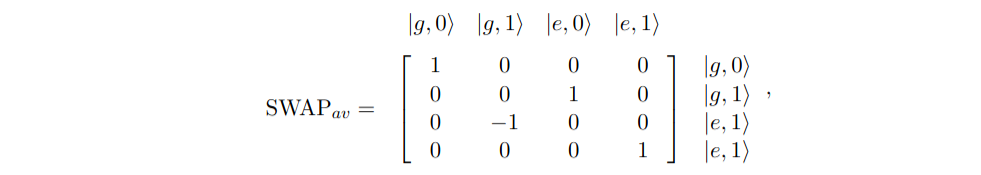
\includegraphics[width=1\linewidth]{Figuras/Fig_ions_SWAPav_matrix.png}
    \caption{Puerta SWAP${}_\text{av}$}
    \label{Fig_ions_SWAPav_matrix}
\end{figure}


con las únicas transiciones no triviales siendo 
	\begin{equation} 
	\begin{aligned}
	\ket{g,1} & \rightarrow - \ket{e,0} \\
	\ket{e,0} & \rightarrow \ket{g,1}
	\end{aligned}
	\end{equation}
La puerta $\text{SWAP}_{av}$ puede implementarse mediante un láser usando la \textit{red sideband resonance}. Utilizando la Fig. (\ref{Fig_ions_U_rsb}), la puerta  $\text{SWAP}_{av}$ puede realizarse mediante la elección de un pulso láser con $\eta \beta = \pi$ y $\phi + \pi/2 = 3 \pi/2$. La inversa de la puerta se puede implementar cambiando la fase del láser a  $\text{SWAP}_{av}$.

		\SubsubiIt{Puerta CZ entre estados atómicos y vibracionales ($\text{CZ}_{av})$}

Se trata de una puerta controlada-Z que actúa sobre los estados atómico y vibracional de un único ion, donde el estado atómico actúa como qubit de control y el estado vibracional actúa como qubit objetivo. En la base de un solo ion
	\begin{equation}
 	\lch \ket{g,0}, \ket{g,1}, \ket{e,0}, \ket{e,1} \rch\, ,
 	\end{equation}
esta puerta se representa como
%\begin{equation} \label{ec_ions_CZav}
% \begin{matrix}
%    & 
    %
%    \begin{matrix}
%      \ket{g,0} & 
%      \ket{g,1} & 
%      \ket{e,0} &
%      \ket{e,1}
%    \end{matrix} 	&  \\[.5\normalbaselineskip]
  %
%    \text{CZ}_{av} = & 
%    \begin{bmatrix}
%        \makebox[\widthof{$\ket{g,0}$}]{$1$} & 
%        \makebox[\widthof{$\ket{g,0}$}]{$0$} & 
%        \makebox[\widthof{$\ket{g,0}$}]{$0$} & 
%        \makebox[\widthof{$\ket{g,0}$}]{$0$} \\
      %
%        \makebox[\widthof{$\ket{g,0}$}]{$0$} & 
%        \makebox[\widthof{$\ket{g,0}$}]{$1$} & 
%        \makebox[\widthof{$\ket{g,0}$}]{$0$} & 
%        \makebox[\widthof{$\ket{g,0}$}]{$0$} \\
      %
%        \makebox[\widthof{$\ket{g,0}$}]{$0$} & 
%        \makebox[\widthof{$\ket{g,0}$}]{$1$} & 
%        \makebox[\widthof{$\ket{g,0}$}]{$0$} & 
%        \makebox[\widthof{$\ket{g,0}$}]{$0$} \\
      %
%        \makebox[\widthof{$\ket{g,0}$}]{$0$} & 
%        \makebox[\widthof{$\ket{g,0}$}]{$0$} & 
%        \makebox[\widthof{$\ket{g,0}$}]{$0$} & 
%        \makebox[\widthof{$\ket{g,0}$}]{$-1$} \\
%    \end{bmatrix} &
%    \begin{matrix} \ket{gg} \\ \ket{ge} \\ \ket{eg} \\ \ket{ee} \end{matrix} 
%\end{matrix} \,,
%\end{equation}
\begin{figure}[h]
    \centering 
    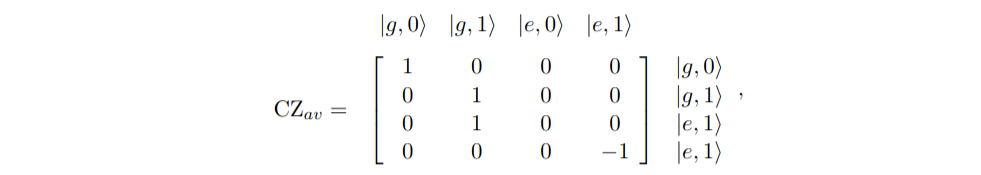
\includegraphics[width=1\linewidth]{Figuras/Fig_ions_CZav_matrix.png}
    \caption{Puerta CZ${}_\text{av}$}
    \label{Fig_ions_CZav_matrix}
\end{figure}


con la única acción no trivial siendo 
	\begin{equation}
	\ket{e,1} \rightarrow - \ket{e,1} \, .
	\end{equation}

Para implementar esta puerta, se busca un nivel auxiliar $\ket{\tilde{e},0}$ del ion que puede alcanzarse \textbf{solo desde} $\ket{e,1}$ mediante un láser de frecuencia $\omega_{e\tilde{e}} + \omega_z$ (ver Fig. \ref{Fig_ions_Niveles_CZav}). Si nos fijamos, la transición
	\begin{equation}
	\ket{\tilde{e},0} \leftrightarrow \ket{e,1}
	\end{equation}
es una transición \textit{blue sideband}, donde cambiamos $g$ por $\tilde{e}$ en la Fig. (\ref{Fig_ions_U_bsb}). Si tomamos la Fig. (\ref{Fig_ions_U_bsb}) para la base 
	\begin{equation}
	\lch \ket{\tilde{e},0}, \ket{\tilde{e},1}, \ket{e,0}, \ket{e,1} \rch.
	\end{equation}
	con $\eta \beta = 2\pi$ y la aplicamos sobre el estado $\ket{e,1}$ obtenemos:
	\begin{equation} 
	\ket{e,1} \rightarrow -\ket{e,1}
	\end{equation}	
Dado que utilizamos un nivel auxiliar para la transición, los demás estados originales no se modifican, lo que da lugar al único cambio no trivial en la Fig. (\ref{Fig_ions_CZav_matrix}).

\Ejercicio{
Comprueba este resultado, es decir, aplica el operador de la Fig. (\ref{Fig_ions_U_bsb}) sobre $\ket{e,1}$ tomando la base $\lch \ket{\tilde{e},0}, \ket{\tilde{e},1}, \ket{e,0}, \ket{e,1} \rch$ y tomando $\eta \beta = 2\pi$.
}


	\begin{figure}[h]
	\centering 
	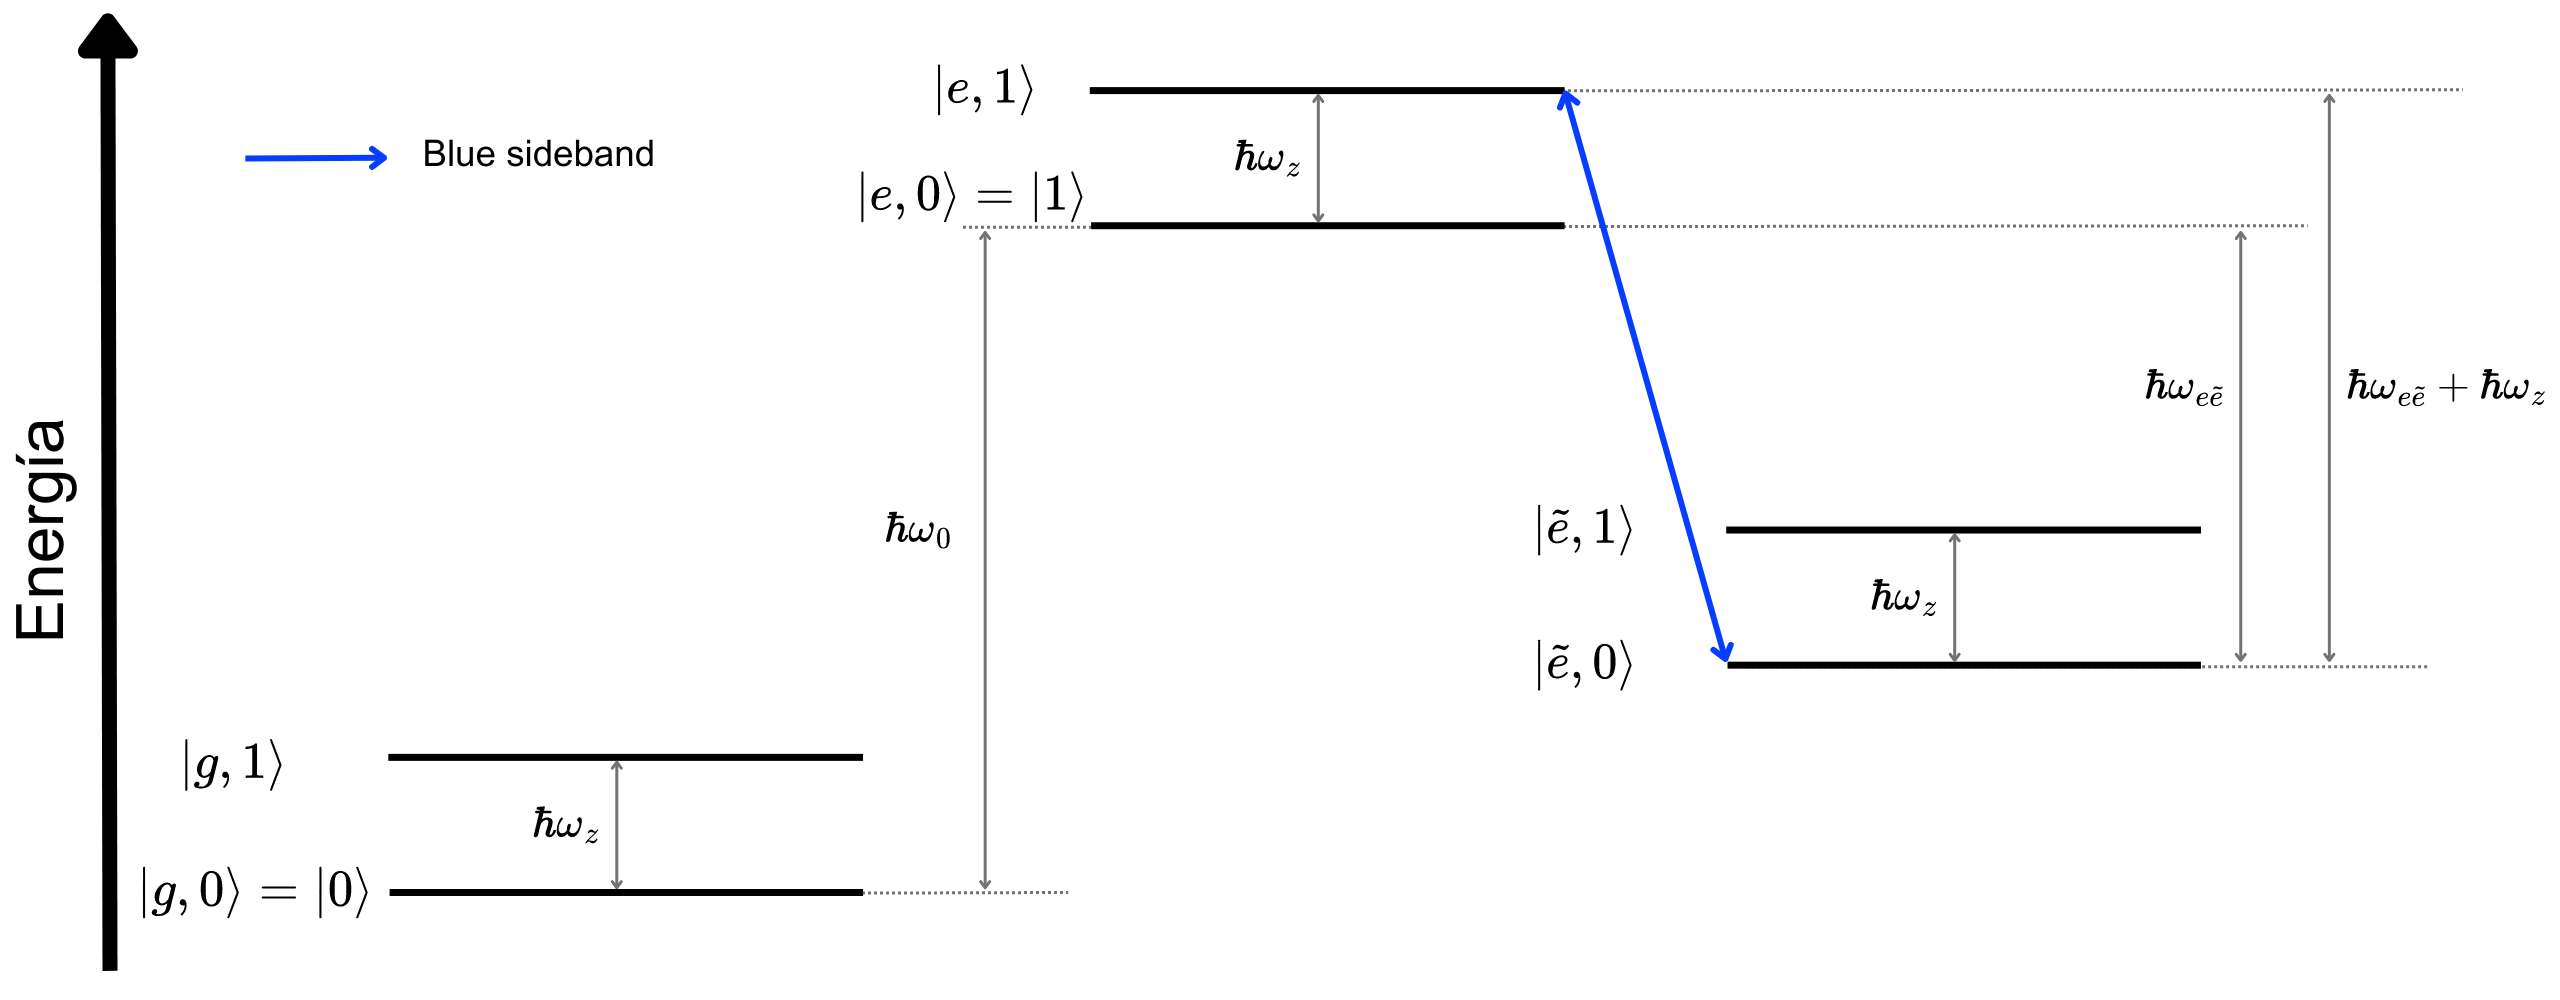
\includegraphics[width=1\linewidth]{Figuras/Fig_ions_Niveles_CZav.png}
	\caption{Nivel auxiliar utilizado para la implementación de la puerta $\text{CZ}_{av}$. Un ion en el estado atómico fundamental ($\ket{g}$) permanece en el estado fundamental debido a la frecuencia fuera de resonancia  del láser para las transiciones de este estado.}
	\label{Fig_ions_Niveles_CZav}
	\end{figure}


\subsection{Implementación de la puerta CZ}

Ahora estamos listos para implementar la puerta CZ para dos iones. El estado más genérico de un sistema de dos iones en el estado fundamental vibracional viene dado por la ecuación
	\begin{equation} \label{ec_ions_psi_2_ions}
	\ket{\Psi_0} = a_{gg} \ket{gg,0} + a_{ge} \ket{ge,0} + a_{eg} \ket{eg,0} + a_{ee} \ket{ee,0} 
	\end{equation}


La puerta CZ puede implementarse en este estado siguiendo paso a paso el siguiente procedimiento (las fuentes en negrita en los siguientes pasos resaltan los cambios en el estado $\ket{\Psi}$)
\begin{itemize}
\item Aplicamos la puerta $\text{SWAP}_{av}$ en el segundo ion:
	\begin{equation}
	\ket{\Psi_1} = a_{gg} \ket{gg,0} + a_{ge} \ket{g\mathbf{e},\mathbf{1}} + a_{eg} \ket{eg,0} + a_{ee} \ket{e\mathbf{g},\mathbf{1}}  
	\end{equation}
	
\item Aplicamos la puerta $\text{CZ}_{av}$ en el primer ion:
	\begin{equation}
	\ket{\Psi_2} = a_{gg} \ket{gg,0} + a_{ge} \ket{ge,1} + a_{eg} \ket{eg,0} - a_{ee} \ket{\mathbf{e}g,\mathbf{1}}  
	\end{equation}
	
\item Aplicamos la inversa de la puerta $\text{SWAP}_{av}$ en el segundo ion:
	\begin{equation}
	\ket{\Psi_1} = a_{gg} \ket{gg,0} + a_{ge} \ket{g\mathbf{g},\mathbf{0}} + a_{eg} \ket{eg,0} - a_{ee} \ket{e\mathbf{e},\mathbf{0}}  
	\end{equation}
\end{itemize}

Obsérvese que tras el conjunto de operaciones descritas anteriormente, el qubit vibracional vuelve al estado fundamental (de donde partió). El qubit vibracional puede eliminarse ahora de la descripción del paso inicial y de final, lo que da la transformación efectiva
	\begin{equation}
	a_{gg} \ket{gg} + a_{ge} \ket{ge} + a_{eg} \ket{eg} + a_{ee} \ket{ee}
	\rightarrow
	a_{gg} \ket{gg} + a_{ge} \ket{ge} + a_{eg} \ket{eg} - a_{ee} \ket{ee}
	\end{equation}
Ahora es evidente que los pasos descritos anteriormente implementan efectivamente la puerta CZ en un sistema de dos iones.


\subsection{La puerta CNOT}

Para implementar la puerta CNOT solo tenemos que tener en cuenta la siguiente relación:
	\begin{equation} \label{ec_ions_CNOT_from_HCZH}
	\text{CNOT} = (\mathbb{I} \otimes H) \text{CZ} (\mathbb{I} \otimes H)
	\end{equation}
(donde la CZ está controlada por el qubit de la izquierda en el par).

Al poder implementar cualquier puerta de un qubit y la CNOT, tenemos un \textbf{conjunto universal de puertas}. Es decir, se cumple el criterio 4 de DiVicenzo (sección \ref{sec_criterio_divicenzo}).

\Ejercicio{
Comprueba la relación de la Ec. (\ref{ec_ions_CNOT_from_HCZH}).
}




\subsection{Creación de los estados de Bell}

Una vez tenemos construidas la CNOT y las puertas de un qubit, podemos construir los estados de Bell como ejemplo para ver que se puede generar entrelazamiento con iones. Construyamos por ejemplo el $B_{00}$ (ver Ec. (\ref{ec_multiqubit_Bell_states}):
	\begin{equation}
	CNOT (H \otimes \mathbb{I}) \ket{gg} = \frac{\ket{gg} + \ket{ee}}{\sqrt{2}}
	\end{equation}




\section{Conclusiones: pros y contras}


A lo largo del capítulo, hemos demostrado que los sistemas de iones atrapados cumplen satisfactoriamente los criterios de DiVincenzo (seccioón \ref{sec_criterio_divicenzo}) para su uso como plataforma para la computación cuántica. En resumen,
\begin{itemize}
\item  Criterios 1(a) y 2: Los qubits de iones atrapados son robustos y pueden inicializarse con gran precisión. 

\item Criterio 3: Los iones tienen una elevada relación entre el tiempo de coherencia ($\sim 10^1$ s) y el tiempo de puerta ($\sim 10^{-6}$ s), lo que da tiempo suficiente para realizar cálculos en el sistema antes de que aparezcan los efectos de la decoherencia.

\item Criterios 4 y 5: Es posible implementar un conjunto universal de puertas y leer iones individuales mediante pulsos láser cuidadosamente ajustados.

\end{itemize}

Además, los iones atrapados pueden entrelazarse fácilmente a pesar de estar físicamente muy alejados, gracias a su manipulación mediante pulsos láser. Se trata de una ventaja significativa con respecto a los qubits superconductores, que convierte a los iones atrapados en una plataforma idónea para simular interacciones de largo alcance, habituales en la física cuántica de muchos cuerpos y en la física de altas energías.

Sin embargo, la escalabilidad (Criterio 1b) a cientos o miles de qubits sigue siendo un reto importante para los iones atrapados. Muchos de los criterios de DiVincenzo se rompen cuando la cadena de iones contiene varios iones. Hay dos dificultades principales:
\begin{itemize}
\item Tiempo de coherencia: Las cadenas de iones más grandes tienen tiempos de coherencia más cortos, y los efectos de la decoherencia son mucho más significativos en cadenas con longitudes de 100 iones o más.

\item Lectura: A medida que la cadena se hace más larga, se hace más difícil leer los iones individuales con alta precisión porque la precisión requerida para que los parámetros del pulso láser midan los iones individuales excede las capacidades tecnológicas actuales.
\end{itemize}

Aparte de los problemas de escalabilidad, el tiempo de puerta absoluto de los iones atrapados es mayor ($\sim 10^{-6}$ s) que el de los qubits superconductores ($\sim 10^{-9}$ s). Por tanto, realizar el mismo cálculo en una plataforma de iones atrapados llevaría mucho más tiempo y supondría un reto para lograr la ventaja cuántica.











\chapter{Computación Cuántica con qubits Superconductores} \label{sec_chapter_hw_scq}


Los qubits superconductores son actualmente la tecnología líder en el espacio comercial de la computación cuántica, siendo explotada o elegida por IBM, Google, Rigetti, Amazon, Alibaba, Baidu, así como por muchas startups como IQM (Finlandia), OQC (Reino Unido), Anyon Systems (Canadá), Alice{\&}Bob (Francia), Nord Quantique (Canadá) y otras. Actualmente es la mejor arquitectura escalable en el modelo basado en puertas, con un récord de 1.121  qubits de IBM (lanzado en diciembre de 2023), aunque, hasta ahora, la calidad de estos qubits sigue siendo insuficiente para que sean útiles en la práctica.

Los qubits superconductores se cimientan en el uso de la \textbf{unión de Josephson} para construir un circuito superconductor que simula un átomo con niveles de energía controlables con precisión. Es decir, los qubit superconductores son \textbf{átomos artificiales}.

En este capítulo vamos a hablar de las uniones de Josephson y de los tipos de qubits superconductores que hay. Después nos centraremos un tipo concreto de qubit superconductor, el \textbf{transmón}, para ver como aplicar operaciones sobre él.

Este capítulo de basa en el articulo de revisión de Olivier Ezratty \cite{bib_scq_ezratty2023perspective}.


\section{Conceptos básicos sobre Superconductividad.}

En esta sección vamos a ver una sería de conceptos que necesitaremos para poder entender como funciona un qubit superconductor. Estos conceptos incluyen que son un superconductor, un par de Cooper y la unión Josephson.


\subsection{Superconductividad}


A temperaturas que la mayoría de la gente considera ``normales", todos los materiales presentan cierta resistencia eléctrica. Esto significa que resisten el flujo de electricidad del mismo modo que una tubería estrecha resiste el flujo de agua. Debido a la resistencia, parte de la energía se pierde en forma de calor. En la mayoría de los materiales, esta resistencia se mantiene aunque el material se enfríe a temperaturas muy bajas. La excepción son los materiales superconductores.

En 1911, mientras estudiaban las propiedades de la materia a muy baja temperatura, el físico holandés Heike Kamerlingh Onnes y su equipo descubrieron que la resistencia eléctrica del mercurio llega a cero por debajo de 4,2 K (-269 °C).  Fue la primera observación del fenómeno de la superconductividad.  

Por debajo de cierta \textbf{temperatura crítica}, ciertos materiales pasan al estado superconductor, caracterizado por dos propiedades básicas: en primer lugar, \textbf{no ofrecen resistencia al paso de la corriente eléctrica}. Cuando la resistencia cae a cero, una corriente puede circular por el interior del material sin disipación de energía. En segundo lugar, siempre que sean suficientemente débiles, los campos magnéticos externos no penetran en el superconductor, sino que permanecen en su superficie. Este fenómeno de expulsión del campo se conoce como \textbf{efecto Meissner}, en honor al físico que lo observó por primera vez en 1933.

La física convencional no explica adecuadamente el estado superconductor, como tampoco lo hace la teoría cuántica elemental del estado sólido, que trata el comportamiento de los electrones por separado del de los iones en la red cristalina. No fue hasta 1957 cuando tres investigadores estadounidenses (John Bardeen, Leon Cooper y John Schrieffer) establecieron la teoría microscópica de la superconductividad.  Según su \textbf{teoría BCS}, los electrones se agrupan en pares mediante la interacción con las vibraciones de la red (los llamados fonones), formando así \textbf{pares de Cooper} que se desplazan por el interior del sólido sin fricción. El sólido puede verse como una red de iones positivos inmersos en una nube de electrones. Cuando un electrón atraviesa esta red, los iones se mueven ligeramente atraídos por la carga negativa del electrón. Este movimiento genera una zona eléctricamente positiva que, a su vez, atrae a otro electrón. La energía de la interacción de los electrones es bastante débil y los pares pueden romperse fácilmente por efecto de la energía térmica; por eso la superconductividad suele darse a muy baja temperatura. Sin embargo, la teoría BCS no explica la existencia de superconductores de alta temperatura a partir de 80 K (-193 °C), para los que hay que recurrir a otros mecanismos de acoplamiento de electrones.



\subsection{Unión de Josephson (Josephson Junction)}

Cuando dos superconductores están bien separados, son bastante independientes y pueden ser tratados por separado. Cuando entre ellos hay un contacto superconductor sustancial, estos forman un único superconductor: se dice que están \textit{fuertemente ligados} (\textbf{strongly linked}). 

Sin embargo, tenemos casos intermedios en los que los electrones (pares de Cooper) pueden fluir de un superconductor a otro, pero de forma tan débil que cada superconductor puede ser visto como esencialmente en equilibro estático. Esto sucede, por ejemplo, cuando los superconductores están separados por una fina capa de un óxido el cual puede ser atravesado por los electrones mediante efecto túnel. También puede ser una fina capa de un metal normal o semiconductor, o un pequeño puente de material superconductor. A este tipo de uniones entre superconductores se las denomina \textbf{uniones Josephson} (\textbf{JJ} de sus siglas en inglés), y fueros descubiertas en 1962 por Brian Josephson \cite{bib_Josephson_1962}.

Supongamos que conectamos los superconductores a los polos de una batería, de forma que aplicamos una diferencia de potencial $V$ en la unión, supongamos que podemos jugar con la batería para hacer variar esta diferencia de potencial. Es decir, la diferencia de potencial es función del tiempo: $V(t)$ . Es estas situaciones tenemos una corriente entre los dos superconductores que está descrita por las \textbf{ecuaciones de Josephson}
\begin{equation} \label{ec_scq_jj}
\begin{aligned}
J &= J_0 \sin \delta \\
\frac{d \delta}{dt} &= \frac{2eV(t)}{\hbar} \, ,
\end{aligned}
\end{equation}
donde $J$ es la densidad de corriente, $e$ es la carga del electrón y $\delta$ es la diferencia de fase entre los dos superconductores $\delta = \theta_1 - \theta_2$. 

\begin{mybox_blue}{Nota: modelo simple de Feynman}
Las ecuaciones (\ref{ec_scq_jj}) pueden derivarse siguiendo un modelo simple del efecto Josephson descrito por Feynman en sus Lectures \cite{bib_scq_Feynman_lectures}. En concreto, puede encontrase online \href{https://www.feynmanlectures.caltech.edu/III_21.html#Ch21-S9}{aquí} o verse en el capítulo ``Superconductivity: Tunneling'' del libro \cite{bib_scq_encyclopedia_of_cmp}.
\end{mybox_blue}

Suponiendo una densidad de corriente uniforme a través del área $A$ de la unión, la corriente total es $I = AJ$, con lo que
	\begin{equation}
	\boxed{I = I_0 \sin \delta} \, .
	\end{equation}
Además, integrando la segunda ecuación de la Ec. (\ref{ec_scq_jj}) tenemos
	\begin{equation}
	\boxed{\delta(t) = \delta_0 + \frac{2e}{\hbar} \int V(t)dt} \,.
	\end{equation}

Aunque la unión Josephson produce varios efectos, vamos a centrarnos en los dos que nos interesan (pueden verse más en \cite{bib_scq_Waldram}):
\begin{itemize}
	\item \textbf{Efecto Josephson de Corriente Continua (DC Josephson effect)}: Si tenemos $V(t)=0$, entonces 
	\begin{equation}
	\delta = \delta_0 \rqa I = I_0 \sin \delta_0
	\end{equation}
	Es decir, cuando no hay diferencia de voltaje en la unión tenemos una \textbf{corriente continua} entre $-I_0$ y $I_0$.
	
	\item \textbf{Efecto Josephson de Corriente Alterna (AC Josephson effect)}: Si tenemos $V(t) = V_0$ constante, entonces
	\begin{equation}
	\delta = \delta_0 + \frac{2eV_0}{\hbar} t \rqa I = I_0 \sin \lp \delta_0 + \frac{2eV_0}{\hbar} t  \rp
	\end{equation}
	Es decir, al aplicar una diferencia de pontecial constante en la unión, aparece una \textbf{corriente alterna} de frecuencia proporcional a la diferencia de potencial.
	
\end{itemize}




\section{Tipos de qubits superconductores}

Veamos ahora a los distintos tipos de qubits superconductores. Estos difieren en la forma de codificar la información cuántica en dos estados distintos. Podemos ver los más importantes en la Fig. \ref{Fig_scq_tipos_qubits_superconductores}

	\begin{figure}[t]
	\centering 
	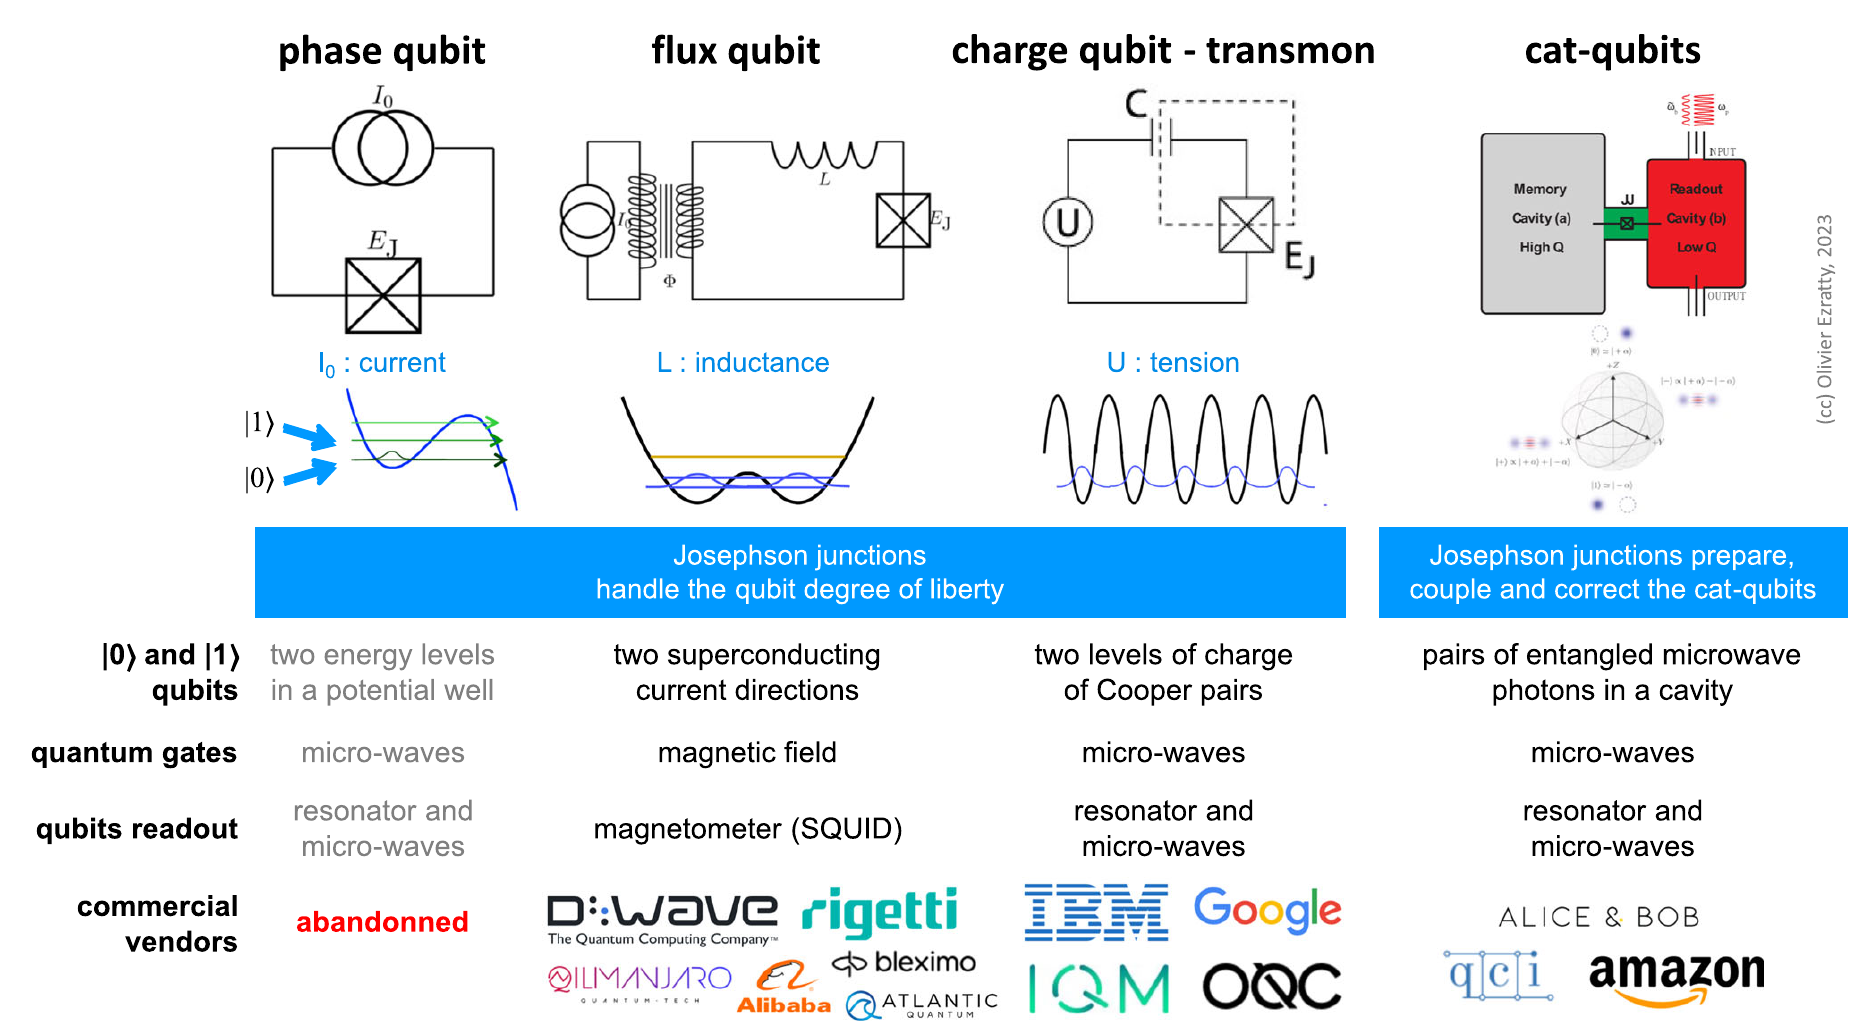
\includegraphics[width=1\linewidth]{Figuras/Fig_scq_tipos_qubits_superconductores.png}
	\caption{Los distintos tipos de qubits superconductores y los proveedores de la industria relacionados. Figura tomada de \cite{bib_scq_ezratty2023perspective}.}
	\label{Fig_scq_tipos_qubits_superconductores}
	\end{figure}




\subsection{Qubits de Carga (Charge Qubits)}

Los \textbf{qubits de carga}, también conocidos como \textbf{cajas de pares de Cooper} (Cooper-pair box), consisten en un circuito superconductor con uniones Josephson, un condensador y una fuente de voltaje. La zona que se forma entre las uniones Josephson y el condensador se denomina \textbf{isla}. Este tipo de circuitos son resonadores LC, donde la unión Josephson hace el efecto de una inductancia \textbf{no lineal}.

El tipo más simple de esta clase de qubits es el que podemos ver en la Fig. \ref{Fig_scq_charge_qubit}, con una sola unión Josephson.  Este consiste en una pequeña isla superconductora (``caja'') con $n$ cargas de pares de Cooper en exceso (en relación con algún estado neutro de referencia), conectada mediante una unión Josephson con capacitancia $C_J$ y energía de acoplamiento Josephson $E_J$ a un electrodo superconductor. Una tensión de control $V_g$ se acopla al sistema a través de un condensador de capacitancia $C_g$. 

	\begin{figure}[b]
	\centering 
	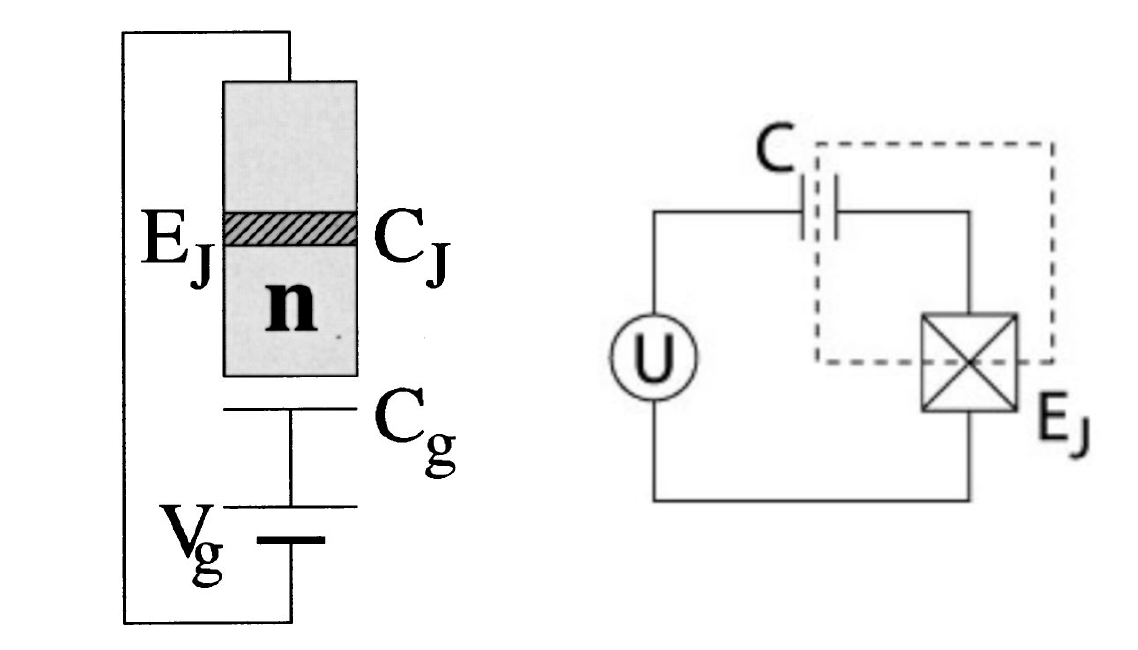
\includegraphics[width=0.5\linewidth]{Figuras/Fig_scq_charge_qubit.png}
	\caption{Forma simple de un circuito superconductor para generar un qubit de carga}
	\label{Fig_scq_charge_qubit}
	\end{figure}

La escala de energía relevante, la energía de carga de un solo electrón $E_C \equiv e^2/2(C_g+C_J)$, que depende de la capacitancia total de la isla, se encuentra en el rango de un Kelvin o superior, $E_C \geq 1 K$ (habitualmente se usan las unidades de temperatura para energía). La energía de acoplamiento Josephson $E_J$ es proporcional a la corriente crítica de la unión Josephson. Los valores típicos considerados aquí están en el rango de $100$ mK ($E_c \gg E_J$). 

Elegimos un material tal que el gap de energía superconductora, $\Delta$, entre el estado fundamental y los estados excitados con cuasiparticulas sea la mayor energía del problema, mayor incluso que la energía de carga de un solo electrón $E_C$. En este caso, el efecto túnel de cuasipartículas se suprime a bajas temperaturas, y se puede llegar a una situación en la que no se encuentre ninguna excitación de cuasipartículas en la isla. En estas condiciones, sólo los pares de Cooper hacen túnel (coherentemente) en la unión superconductora. 

Es decir, las únicas excitaciones de baja energía son las transiciones entre diferentes estados $\ket{n}$ (donde $n$ es el número de pares en la isla respecto a un estado neutro de referencia) debido a efecto túnel de pares de Cooper en la unión Josephson. 

La inductancia no lineal de la unión Josephson hace que el resonador LC sea ligeramente anarmónico. Es decir, a diferencia del oscilador armónico cuántico que presenta unos niveles de energía \textbf{equiespaciados}, la presencia de una inductancia no lineal hace que los niveles de energía dejen de estar equiespaciados. Esto permite que podamos coger los dos de menos energía como los estados de nuestro qubit sin miedo a que se nos den transiciones a niveles de energía superiores. Podemos ver esto en la Fig. \ref{Fig_scq_LC_energy_levels}. Explicaremos más en detalle este fenómeno en la sección \ref{sec_scq_fisica_de_lo_scq}.


	\begin{figure}[t]
	\centering 
	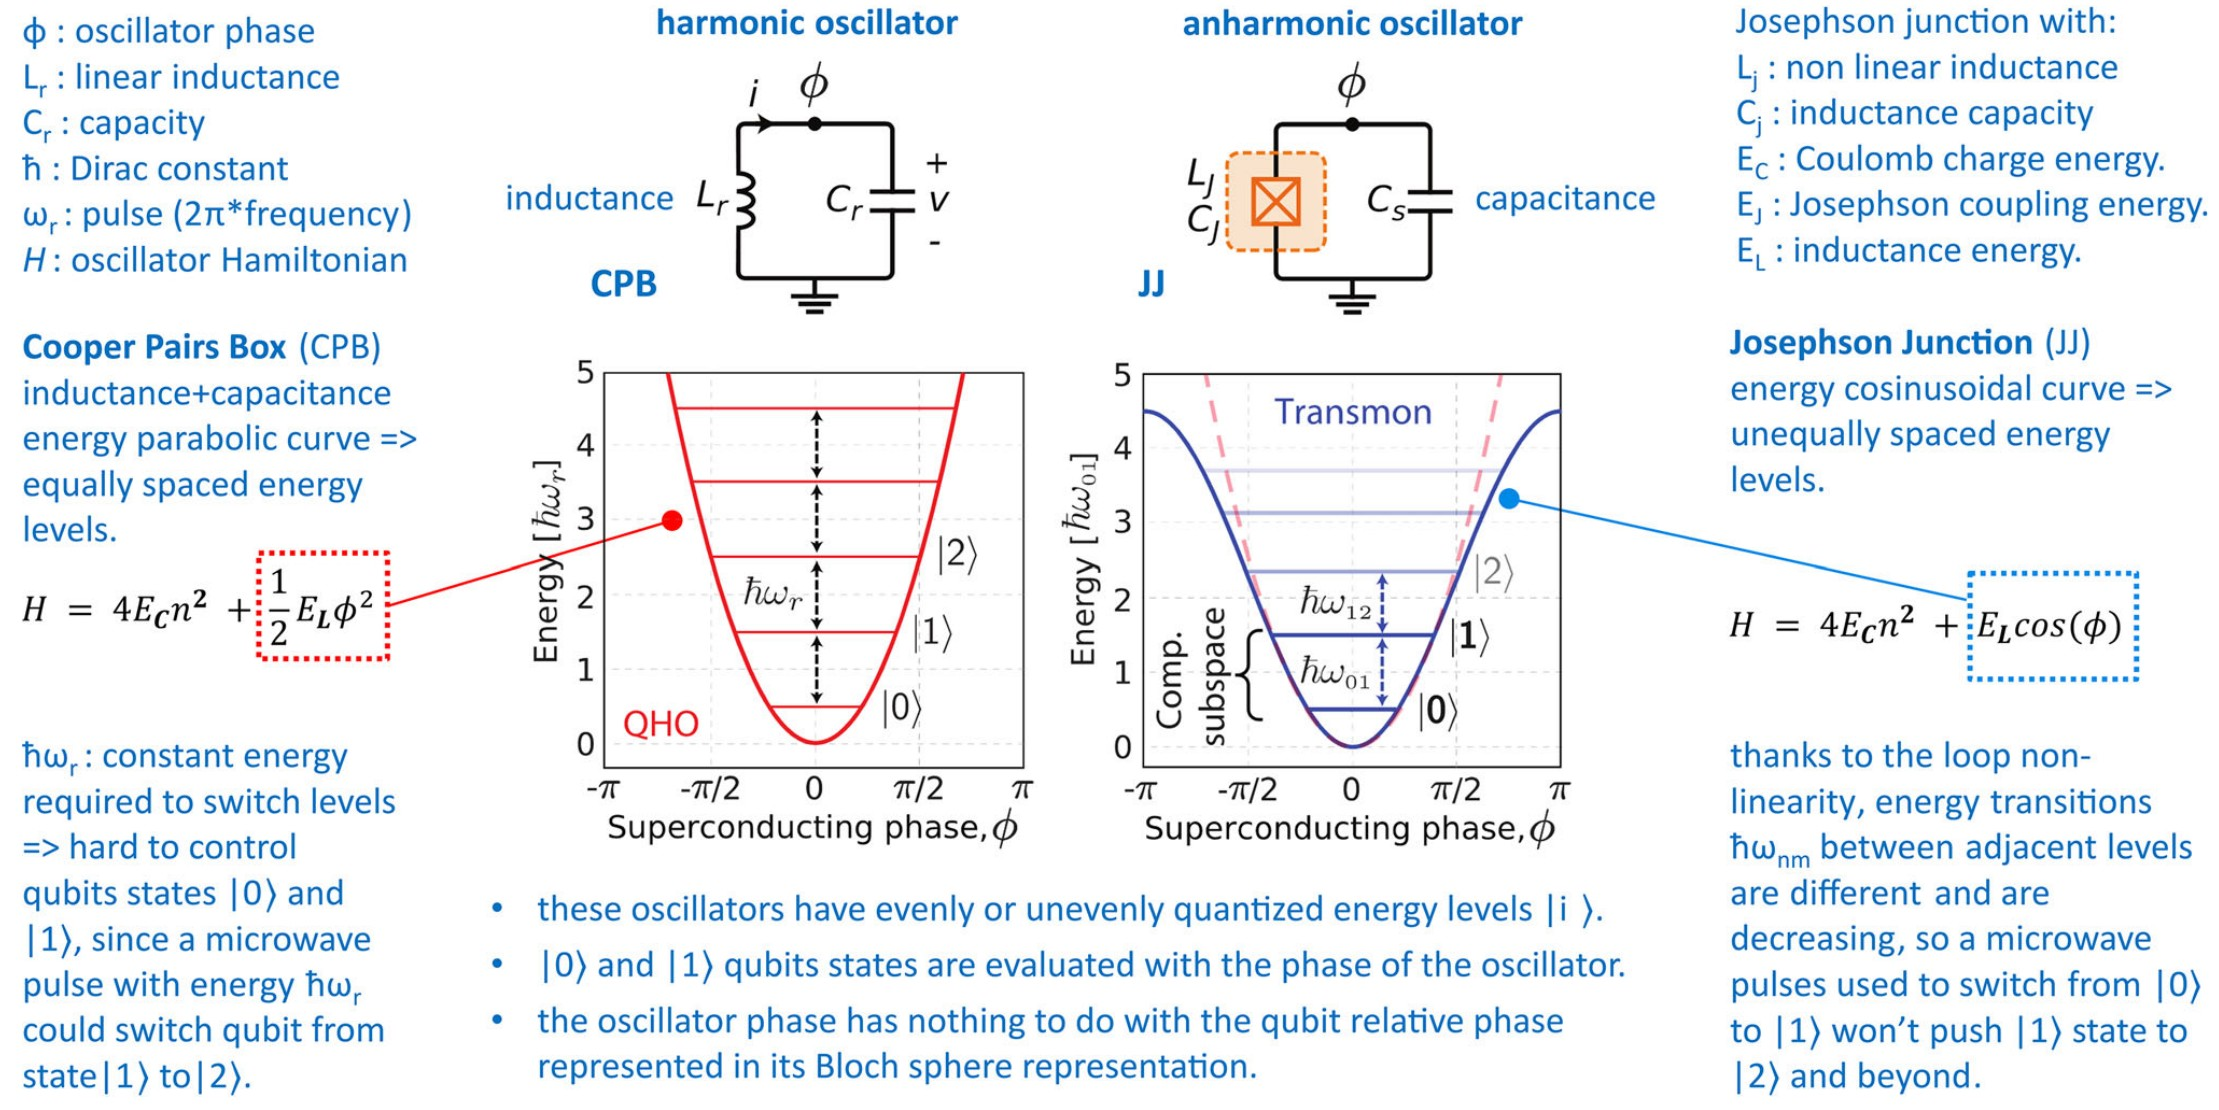
\includegraphics[width=1\linewidth]{Figuras/Fig_scq_LC_energy_levels.jpeg}
	\caption{Diferencia en los niveles de energía entre un oscilador armónico (circuito LC) y un oscilador anarmónico (circuito con un condensador y una unión Josephson). Figura tomada de \cite{bib_scq_ezratty2023perspective}}
	\label{Fig_scq_LC_energy_levels}
	\end{figure}

La variante más común es el \textbf{transmón}, por ``transmission line shunted plasma oscillation qubit'', que reduce el efecto del ruido de carga pero con una anarmonicidad más débil. Los transmones son utilizados por IBM, Google, IQM y otros. Hasta la fecha, son los qubits que generan la \textbf{tasa de error más baja en los qubits superconductores}, pero su baja anarmonicidad crea un peaje en las velocidades de puertas y lectura.

Se dividen en al menos dos categorías: qubits con \textbf{una sola unión Josephson} (transmón de unión simple, utilizado por IBM) o con \textbf{dos uniones Josephson} conectadas en paralelo (\textit{spit transmon}, utilizado por Google). 

Además, existen muchas variaciones con el coaxmon (OQC) y el unimon (IQM) y el mergemon o transmon de elemento fusionado, en el que la unión Josephson está diseñada para actuar como su propio condensador de derivación paralelo, reduciendo el tamaño del qubit.


\subsection{Qubits de Flujo (Flux Qubits)}

Los estados de los \textbf{qubits de flujo} corresponden a la dirección del flujo de la corriente superconductora en su bucle. Acoplan un condensador, de una a tres uniones Josephson y un superinductor y tienen una gran coherencia y una gran anarmonicidad.

Para medir el estado de un qubit de este tipo se utiliza un SQUID (dispositivo superconductor de interferencia cuántica) con dos uniones Josephson conectadas en paralelo, un magnetómetro que mide la dirección de la corriente en el qubit y, por tanto, su estado fundamental 0 ó 1.

Este tipo de qubit superconductor es el adoptado por D-Wave, Rigetti, Alibaba, Bleximo y Atlantic Quantum en el espacio de vendedores de la industria.

En trabajos recientes, los qubits de fluxonio generaron el mejor $T_1 /T_2$ con $T_1$ superior a 1 ms. Utilizan frecuencias de control normalmente inferiores a 3 GHz, lo que reduce los efectos de pérdida dieléctrica y da lugar a un tiempo de relajación $T_1$ prolongado. Las puertas single-qubit pueden tener un tiempo de aplicación en el rango de 10 ns y niveles de error alrededor de $10^{-4}$. En esta arquitectura, se espera que tanto la interferencia (crosstalk) de lectura como la de control sean pequeñas. Las principales deficiencias de los qubits de flujo son su mala protección frente a la relajación ($T_1$) y el desfase ($T_2$) y la complejidad del circuito para las puertas y la lectura.

Por último, en el ámbito del annealing cuántico, D-Wave está utilizando SQUIDs controlados por flujo que se acoplan magnéticamente para implementar un proceso de annealing cuántico. La empresa tiene previsto implantar qubits de flujo en un modo basado en puertas, con diseños de chip completamente distintos.


\subsection{Otros tipos de qubits superconductores} 

		\SubsubiIt{Qubits de Fase (Phase Qubits)}

Los qubits de fase utilizan uniones Josephson más grandes que en los qubits de carga. Su estado corresponde a dos niveles de energía de corriente en una unión Josephson. Este enfoque fue probado por el NIST en EE.UU., entre otros lugares, pero ningún vendedor comercial parece utilizar este tipo de qubit superconductor. El qubit de fase parece un callejón sin salida.



		\SubsubiIt{Qubits de espín Andreev (ASQ)}

\textbf{Andreev Spin Qubits (ASQ)} es un qubit de nivel de investigación que se basa en una excitación microscópica localizada del condensado BCS que de forma nativa sólo tiene dos niveles y se basa en un nanocable. No se trata de una excitación colectiva del circuito de bucle superconductor. Dado que manipula los espines de los electrones en relación con un resonador superconductor y utiliza la electrodinámica de circuitos (cQED), se sitúa entre las categorías de qubits de espín superconductores y de silicio.

		\SubsubiIt{Cat-qubit}

Los \textbf{cat-qubits} son qubits basados en cavidades conectados a un qubit transmón que se utiliza únicamente para su preparación, lectura y/o corrección, dependiendo de la implementación.

		\SubsubiIt{Qubits Bosónicos}

Los \textbf{qubits bosónicos} son una amplia categoría de qubits resistentes al ruido o que generan menos ruido y permiten ensamblar qubits lógicos con muchos menos qubits físicos, en el rango de 10-100 en lugar de 1000-10.000. Contiene cat-qubits y códigos GKP.

El enfoque cat-qubits es el elegido por Alice{\&}Bob (Francia), Amazon (EE.UU.) y QCI (EE.UU.), mientras que Nord Quantique (Canadá) parece utilizar otra clase de código bosónico.




\section{Física de los qubits superconductores} \label{sec_scq_fisica_de_lo_scq}

Nos centraremos aquí en los qubits transmones, que son los más comunes, siendo explotados por IBM, Google e IQM. 

Estos qubits son osciladores anarmónicos y, por tanto, no lineales. Su no linealidad procede de la unión Josephson. Esta no linealidad es la que hace que los estados de energía no estén equiespaciados (a la derecha en la Fig. \ref{Fig_scq_LC_energy_levels}), como si sucede cuando tenemos un resonador lineal formado por un condensador y una inductancia (una bobina) (\textbf{circuito LC}, a la izquierda en la Fig. \ref{Fig_scq_LC_energy_levels}). Este circuito LC se comporta como un \textbf{oscilador armónico}. En un oscilador armónico, los niveles de energía están espaciados por igual y son múltiplos del primer nivel de energía ($\hbar \omega_r$ en el diagrama). En el transmón, la unión Josephson tiene una inductancia no lineal que crea su anarmonicidad. En ambos casos, la corriente que fluye está cuantizada con niveles de energía discretos correspondientes a las barras horizontales del gráfico de la Fig. \ref{Fig_scq_LC_energy_levels}.


\begin{mybox_blue}{Nota: El circuito LC}
Un Circuito LC, también denominado circuito resonante u oscilador LC, es un circuito eléctrico formado por una bobina, representado por la letra L y un condensador, representado por la letra C, los cuales se encuentran conectados entre sí. El circuito actúa como un resonador eléctrico a la frecuencia de resonancia del circuito.
\vspace{0.3cm}

Al estar el condensador y la bobina en paralelo, la energía almacenada por el campo eléctrico del condensador (en forma de cargas electrostáticas), es absorbida por la bobina, que la almacena en su campo magnético, pero a continuación es absorbida y almacenada por el condensador; nuevamente en forma de campo eléctrico; para ser nuevamente absorbida por la bobina, y así sucesivamente.
\vspace{0.3cm}

Es decir, tenemos un condensador que almacena energía eléctrica, en el sentido de que un lado del condensador tiene carga positiva y el otro carga negativa. En esta situación, la tendencia del circuito es a equilibrar la carga entre los dos lados del condensador, ``liberando'' la energía almacenada. De esta forma, la carga negativa fluye por el circuito hacía la cara cargada positivamente, generando una corriente. 
\vspace{0.3cm}

Si el condensador estuviera solo en el circuito, simplemente se descargaría. Sin embargo, la presencia de la bobina (inductancia) hace que al haber una corriente se genere un campo magnético que a su vez genera un campo eléctrico que arranca más electrones de la cara negativa del condensador. El resultado esta vez es que, en vez de alcanzar el equilibrio de carga en el condensador, lo que pasa es que la cara que antes estaba cargada positivamente, ahora está cargada negativamente, y viceversa con la otra cara. Es decir, la carga del condensador se ha invertido. Estamos en la misma situación del principio pero con la carga invertida, así que sucederá lo mismo, pero está vez la corriente irá en sentido inverso.
\vspace{0.3cm}

Este ciclo se irá repitiendo, generando una corriente que oscila a una frecuencia determinada por los valores de la inductancia $L$ y del capacitancia $C$.
\end{mybox_blue}

 

Estos estados de energía suelen controlarse mediante pulsos de microondas en el régimen de 5 GHz. Estos pulsos se atenúan mucho para dejar pasar muy pocos fotones. Estas interacciones entre qubits superconductores y fotones de microondas forman parte de una rama de la física cuántica denominada \textbf{electrodinámica cuántica de circuitos}, o \textbf{cQED} de sus siglas en inglés.

Como podemos ver en la derecha en la Fig. \ref{Fig_scq_LC_energy_levels}, la diferencia de energía entre los niveles se va haciendo más pequeña a medida que subimos de nivel. Nosotros para los estados $\ket{0}$ y $\ket{1}$ cogemos los dos estados de menor energía del sistema (los dos inferiores). La energía de transición $\hbar \omega_{01}$ entre los estados $\ket{0}$ y $\ket{1}$ es superior a las energías de transición $\hbar \omega_{12}$, $\hbar \omega_{23}$, $\dots$, entre los niveles superiores.  

Si los niveles de energía estuvieran equiespaciados, al enviar un pulso (fotones) con la energía de transición entre los dos estados de nuestro qubit, este pulso podría hacer promocionar el qubit a estados de energía superiores. Al no estar equiespaciados, nuestro pulso solo puede afectar a la transición deseada. Esto es debido a que en física cuántica las transiciones solo se dan sí se le aporta al sistema la energía justa de la transición. Para que se dieran transiciones a estados de energía superiores, tendríamos que aplicar un pulso diferente, con otra energía.


Los qubits superconductores que se controlan con pulsos en torno a $\omega_{01} \approx 5$ GHz, tiene una energía de transición equivalente a una temperatura de unos 250 mK, muy superior a la temperatura de 15 mK utilizada habitualmente. Es decir, si nuestro qubit con $\omega_{01} \approx 5$ GHz estuviera a una temperatura 250 mK o superior, la transición entre los estados podría darse de forma espontánea. 

Hay otra razón para hacer funcionar el qubit a unos 15 mK. Se necesita una cierta cantidad de energía para romper los pares de Cooper de un qubit superconductor. En el aluminio, que es el material típico utilizado para crear la unión Josephson y sus alrededores, esta energía corresponde a 90 GHz a 20 mK. Es un orden de magnitud mayor que la diferencia de energía entre los dos niveles de un qubit. Esto significa que el qubit puede ser manipulado con energías más bajas (en el rango de 4-8 GHz) sin que se rompan los pares de Cooper de la corriente superconductora y se altere la coherencia cuántica del qubit. 


El qubit se acopla a una cavidad que contiene un \textbf{resonador de lectura}, generalmente implementado como un resonador de \textbf{guía de onda coplanar} (CPW de sus siglas en inglés) en un circuito superconductor. Su longitud suele corresponder a un cuarto de longitud de onda del resonador. Con una frecuencia de accionamiento de 6 GHz, se convierte en un resonador de 1,25 cm que suele apretarse en un trazado serpenteante. Este resonador se utiliza para \textbf{medir el estado del qubit}. Podemos ver un ejemplo de un chip superconductor de 7 qubits en la Fig. \ref{Fig_scq_chip_7_qubits}

	\begin{figure}[t]
	\centering 
	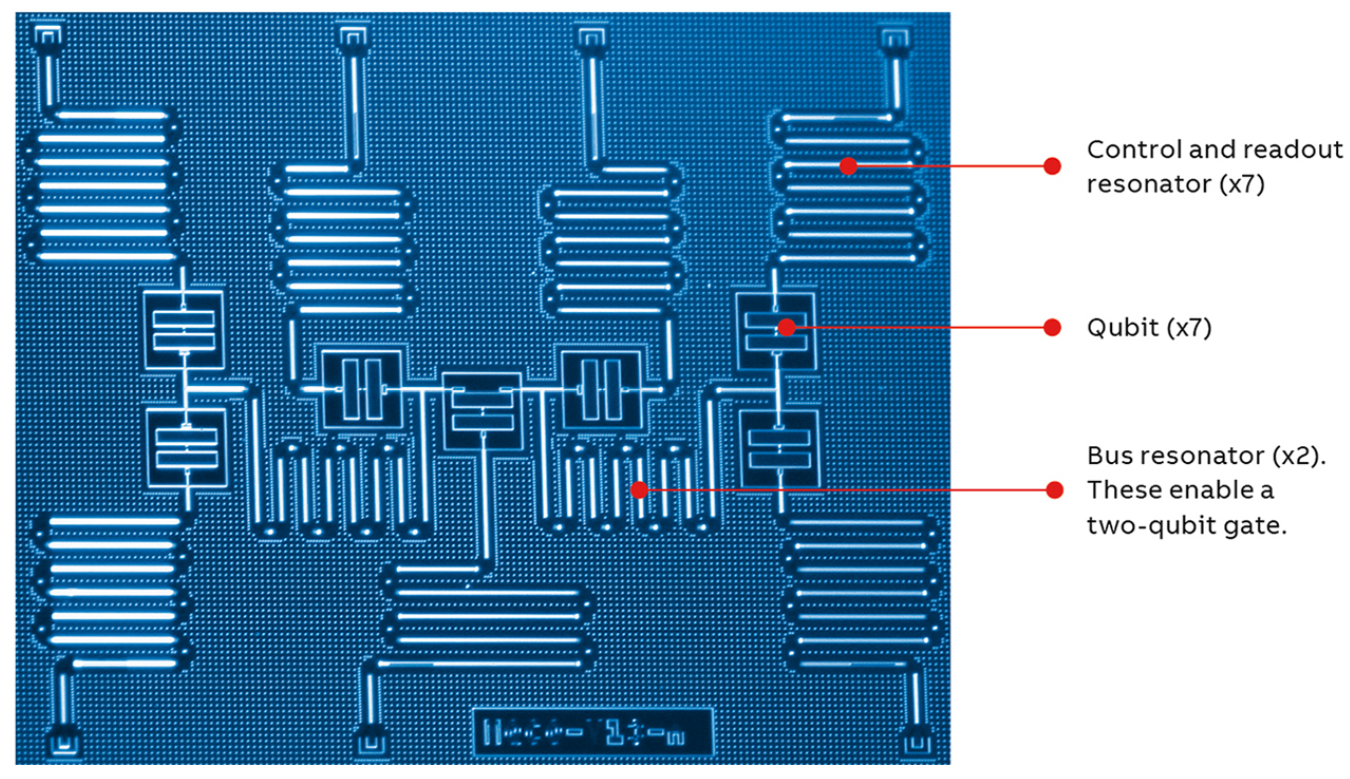
\includegraphics[width=0.7\linewidth]{Figuras/Fig_scq_chip_7_qubits.png}
	\caption{Chip superconductor de 7 qubit diseñado por IBM.}
	\label{Fig_scq_chip_7_qubits}
	\end{figure}










\section{Operaciones con qubits superconductores}

El principio general de funcionamiento de los transmones (qubits superconductores) es el siguiente:


\subsection{Estado del qubit transmón}

\textbf{El estado cuántico del qubit} en el caso genérico de un transmón es un sistema de dos niveles de carga de pares de Cooper que corresponden a un oscilador no lineal que contiene al menos una unión Josephson y una capacitancia. Es decir, los estados se diferencian por el número de pares de Cooper en la isla (en concreto, en un par). Hay casos donde la frecuencia de resonancia del qubit puede ser ajustada con un pulso de corriente continua, lo que ayuda a reducir la interferencia (\textit{crosstalk}) entre qubits, pero a costa de un menos tiempo de vida $T_1$. Por eso lo más común es tener frecuencias de qubit fijas y diferentes.

\subsection{Puertas de un qubit}

Las puertas cuánticas de un solo qubit se generan mediante pulsos de microondas enviados a través de cables coaxiales sobre los qubits (Fig. \ref{Fig_scq_pulsos_1}). Su frecuencia se ajusta al nivel de energía $\hbar \omega_{01}$ mencionado anteriormente. Esta frecuencia se calibra para que sea diferente en qubits adyacentes para evitar efectos de \textit{crosstalk}. La \textbf{amplitud} del pulso de microondas controla el \textbf{ángulo de rotación} y su \textbf{fase} ajusta el \textbf{eje} de la operación de rotación de la puerta. 

	\begin{figure}[t]
	\centering 
	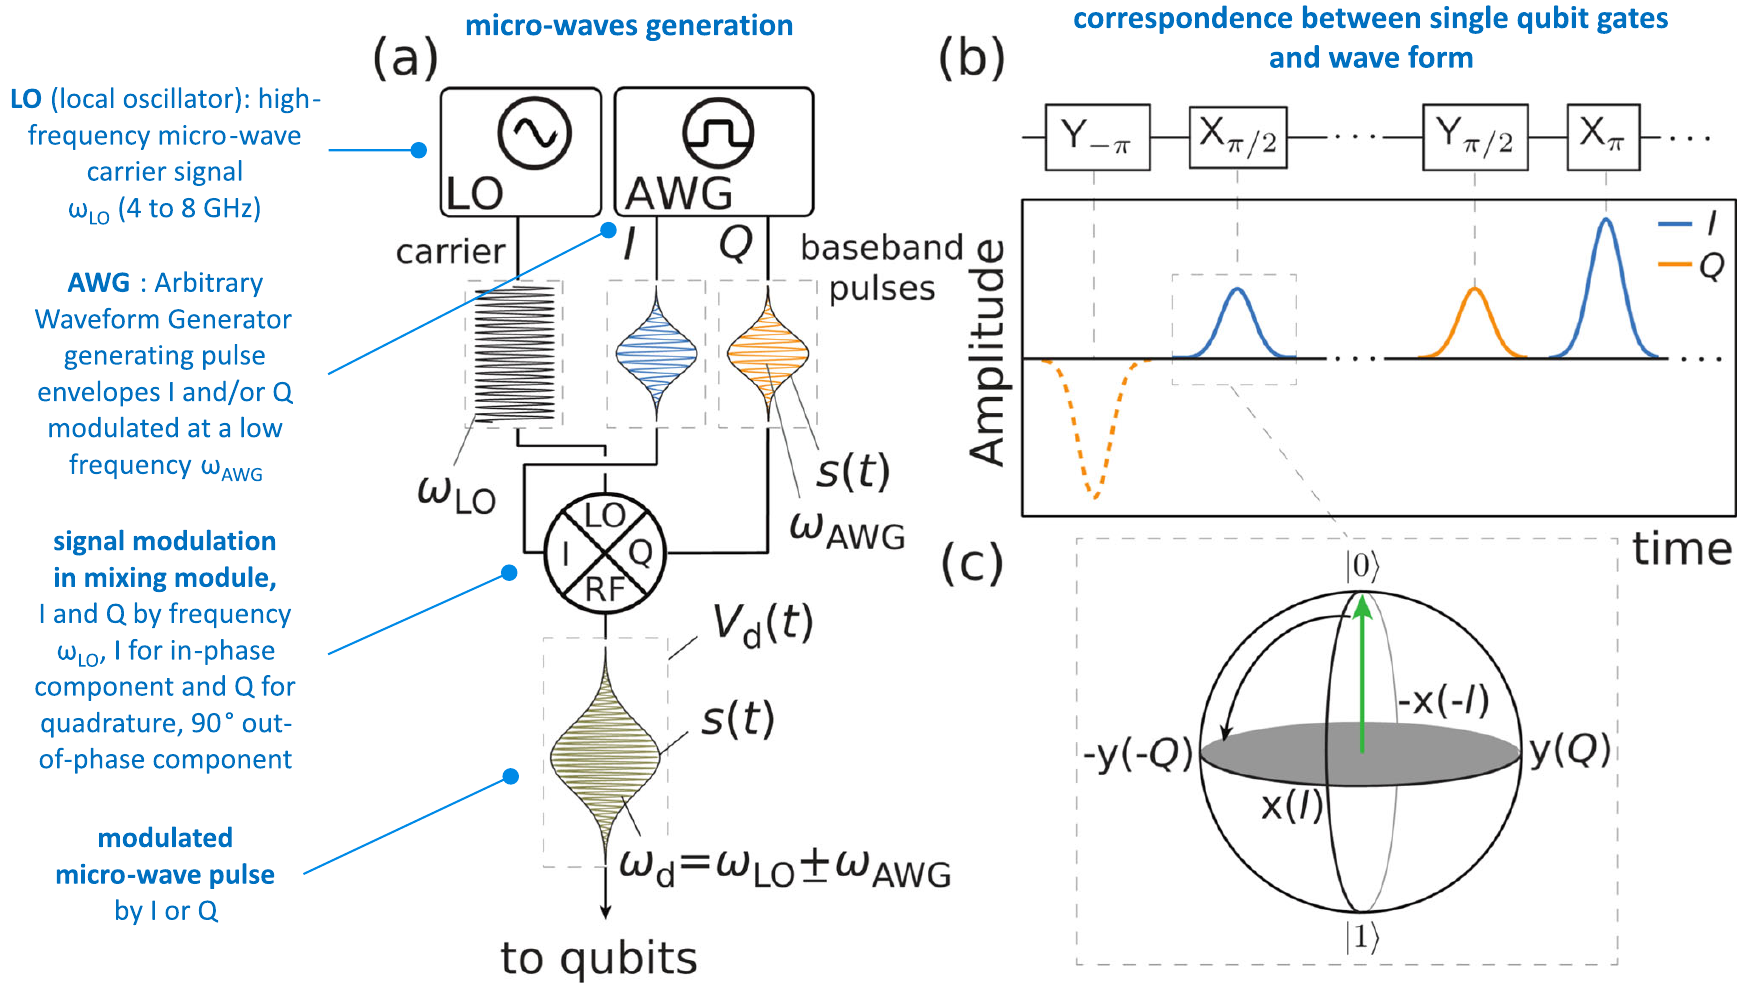
\includegraphics[width=1\linewidth]{Figuras/Fig_scq_pulsos_1.png}
	\caption{a) Esquema de una configuración típica de control de un qubits. Una fuente de microondas suministra una señal de alta frecuencia ($\omega_{LO}$), mientras que un generador de onda arbitrarios (AWG de sus siglas en inglés) suministra una envolvente del pulso ($s(t)$), a veces con un componente de baja frecuencia, $\omega_{AWG}$. El mezclador $IQ$ combina las dos señales para generar una forma de onda $V_d(t)$ con una frecuencia $\omega_d = \omega_{LO} \pm \omega_{AWG}$, normalmente resonante con el qubit. b) Ejemplo de cómo una secuencia de puerta se traduce en una forma de onda generada por el AWG. Los colores indican los componentes $I$ y $Q$. c) La acción de un pulso $X_{\pi/2}$ sobre un estado $\ket{0}$ para producir el estado $\ket{-i} = \frac{1}{\sqrt{2}} (\ket{0} - i\ket{1})$. Figura tomada de \cite{bib_scq_ezratty2023perspective}}
	\label{Fig_scq_pulsos_1}
	\end{figure}

	\begin{figure}[t]
	\centering 
	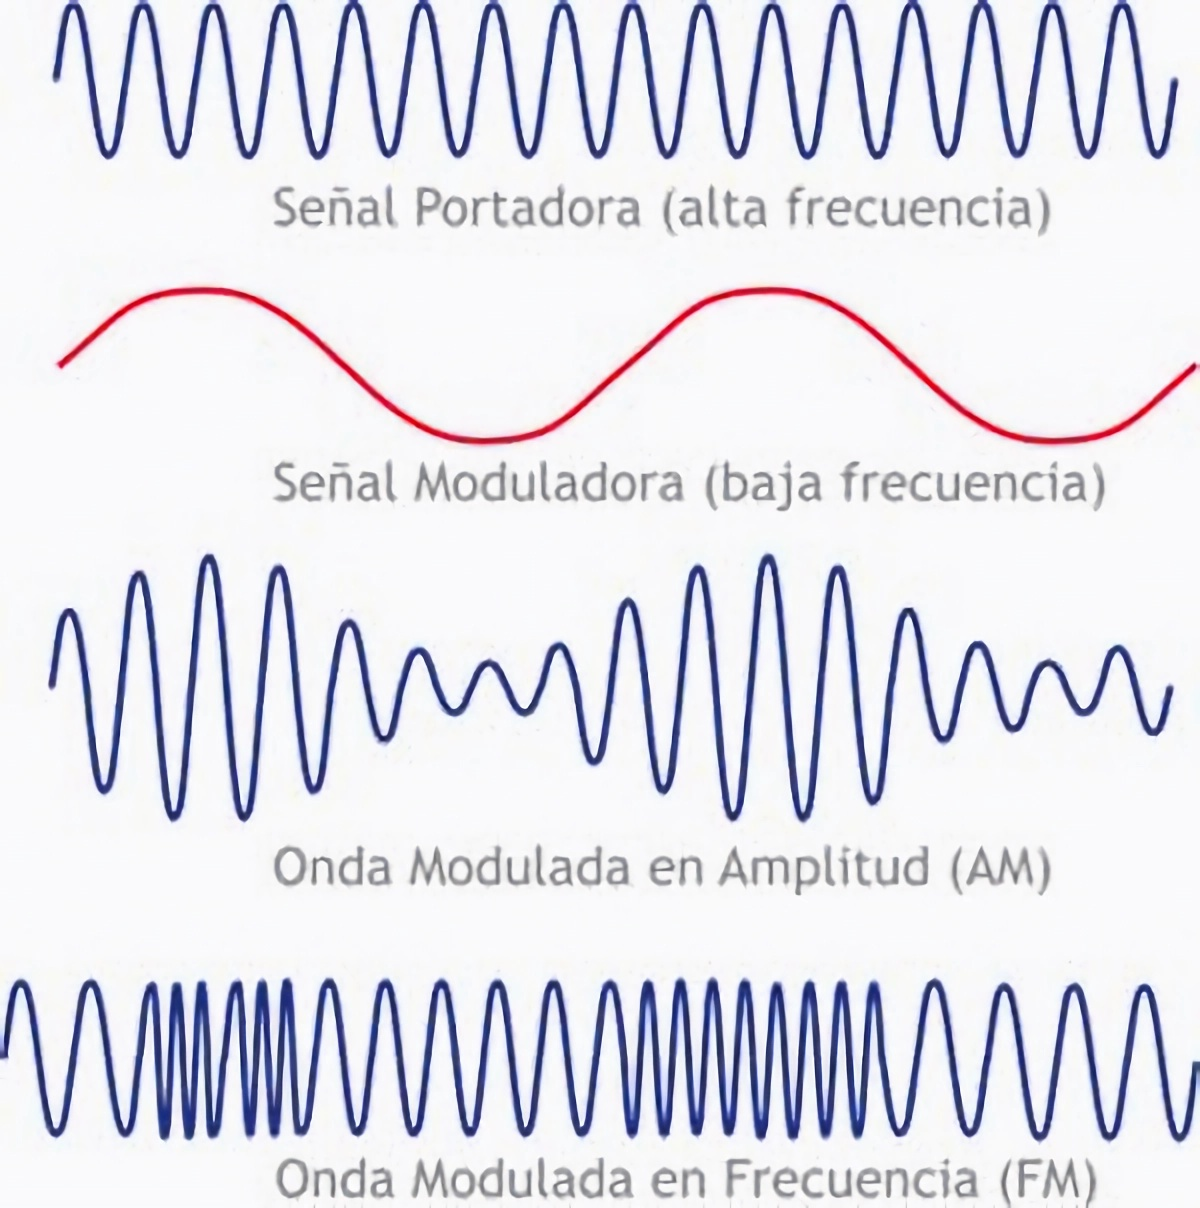
\includegraphics[width=0.4\linewidth]{Figuras/Fig_scq_modulacion.jpg}
	\caption{Ejemplos de ondas moduladas, tanto en amplitud (lo que se usa en control de qubits y en la radio AM), como en frecuencia (lo que usa en las radios FM). Como vemos tenemos dos ondas, la \textbf{portadora} y la \textbf{moduladora}. La gracia aquí es que la información que se quiere transmitir está en la onda moduladora. Esta puede ser, por ejemplo, la onda del sonido que tiene que emitir la rádio del coche. La onda portadora se usa para transmitir la información de la moduladora.}
	\label{Fig_scq_modulacion}
	\end{figure}

El pulso $V_d(t)$ podemos escribirlo de forma genérica como:
\begin{equation} \label{eq_scq_Vd_1}
V_d(t) = V_0 v(t) = V_0 s(t) \sin(\omega_d t + \phi) \, ,
\end{equation}
es decir, como un pulso senoidal de frecuencia $\omega_d$ con un desfase $\phi$ modulado por una función adimensional $s(t)$ denominada \textbf{envoltura}. (Puede verse más sobre modulación de señales en la Fig. \ref{Fig_scq_modulacion}). La frecuencia $\omega_d$ será la frecuencia de resonancia del qubit. Puede verse este pulso en la Fig. \ref{Fig_scq_pulsos_1}a. Usando la identidad trigonométrica del seno de la suma, podemos reescribir el pulso como:
	\begin{equation}
	V_d(t) = V_0 s(t) \Lc \cos(\phi) \sin(\omega_d t) + \sin(\phi) \cos (\omega_d t) \Rc
	\end{equation}
Adoptando las definiciones:
\begin{equation} 
\begin{aligned}
I & = \cos (\phi) \quad (\text{componente ``en-fase''}) \\
Q & = \sin (\phi) \quad (\text{componente ``fuera-de-fase/quadratura''})
\end{aligned}
\end{equation}
con lo que llegamos a:
	\begin{equation} \label{eq_scq_Vd_2}
	\boxed{V_d(t) = V_0 s(t) \Lc I \sin(\omega_d t) + Q \cos (\omega_d t) \Rc}
	\end{equation}
Vemos que si $\phi = 0$, tenemos $V_d(t) = V_0 s(t) \sin(\omega_d t)$ y si $\phi = \pi/2$ tenemos $V_d(t) = V_0 s(t) \cos(\omega_d t)$. 




Como dijimos, la Eq. \ref{eq_scq_Vd_1}, que acabamos reescribiendo como la Eq. \ref{eq_scq_Vd_2}, describe la forma genérica de un pulso de control de un qubit. La pregunta ahora es, como generamos este pulso? En la práctica, se usan dos generadores de ondas y un mezclados:
\begin{itemize}
	\item Tenemos un \textbf{generador de ondas arbitrario} (\textbf{AWG}, de sus siglas en inglés) que crea dos ondas, una denominada ``en fase'' y otra denominda ``cuadratura/fuera-de-fase'' ($I$ y $Q$) que son dos pulsos de microondas sinusoidales que tienen la misma frecuencia $\omega_{AWG}$, están desfasados 90º (uno un seno y otro un coseno) y están modulados por una envolvente $s(t)$. 
	\item Tenemos un generador que denominados \textbf{oscilador local} (\textbf{LO}, de sus siglas en inglés) que genera una onda sinusoidal de frecuencia $\omega_{LO}$.
	\item Finalmente tenemos un mezclados que compone las tres ondas para dar una onda de frecuencia $\omega_d = \omega_{LO} \pm \omega_{AWG}$, modulada con la envolvente $s(t)$ y con una fase arbitraria $\phi$. Esta fase depende de las amplitudes relativas de las ondas $I$ y $Q$. 
\end{itemize}
Habitualmente tenemos que $\omega_{LO} \gg \omega_{AWG}$. Además, recordar que $\omega_d = \omega_{LO} \pm \omega_{AWG}$ debe de ser la frecuencia de resonancia del qubit, que ronda los $5$ GHz, así que $\omega_{LO}$ suele estar próxima.

Como ya dijimos, la \textbf{amplitud} del pulso de microondas controla el \textbf{ángulo de rotación} y su \textbf{fase} el \textbf{eje} de rotación. Esto se traduce en que la fase $\phi$ que ajustamos con las ondas $IQ$ controla el eje, mientras que la envolvente $s(t)$ que aplicamos al pulso controla la rotación.

Los pulsos de microondas generados a temperatura ambiente se atenúan y filtran progresivamente en cada etapa del criostato, de modo que sólo llegan al qubit un par de centenares de fotones de microondas.


\subsection{Puertas de dos qubits}

Las puertas cuánticas de dos qubits se realizan con un \textbf{circuito de acoplamiento} situado entre los dos qubits, que puede ser un simple condensador o un sistema controlable dinámicamente. Dependiendo de la implementación, existen varios tipos de puertas de dos qubits, como la $\sqrt{\text{iSWAP}}$ o la puerta CZ. Este acoplamiento se gestiona con un qubit intermedio en el procesador Sycamore de Google y sus equivalentes chinos. IBM no utiliza acopladores, sino puertas de resonancia cruzada (\textbf{cross-resonance gates}).



\subsection{Lectura de los qubits}

La lectura de los qubits depende de su tipo. Con los qubits transmon, se acopla un resonador al qubit. Este resonador suele tener forma de serpenteánte en zig-zag. 

Por este resonador se transmite un impulso de microondas que es reflejado al llegar al qubit. Estas microondas reflejadas suelen amplificarse en varias etapas. El método se denomina ``lectura dispersiva'': para una frecuencia de microondas fija, la frecuencia de resonancia del resonador de guía de ondas cambia en función del estado del qubit medido. Es decir, el estado del qubit afecta ligeramente a la frecuencia y la fase del pulso reflejado. La medición de la fase de la microonda reflejada determina el estado del qubit tras la medición sin destruirlo.  


\subsection{Conectividad.}

La conectividad es una característica importante de un procesador cuántico. Cuantos más qubits estén conectados entre sí, menos puertas SWAP habrá que ejecutar para entrelazarlos lógicamente.

Con las estructuras 2D, uno de los problemas a resolver radica en las conexiones internas del chipset. Estas topologías consisten en una única capa de metal sobre la oblea de qubits y una placa de circuito impreso. Aunque este esquema funciona bien para topologías en anillo (aquellas en las que los qubits están dispuestos en un anillo), se rompe si hay qubits en el centro del anillo porque no hay forma forma de enviarles señales de microondas. 

También tenemos la arquitectura 3D con dos capas. Esta consiste en dos chips separados, cada uno con una capa de metal estampado, unidos por uniones superconductoras: una capa para la lectura de qubits (oblea intercalada) y otra para las operaciones con qubits. Este esquema permite llevar las señales de microondas al centro del chip de qubits, ``rompiendo el plano''. 

\begin{mybox_blue}{Nota: Los proceadores Falcon y Hummingbird de IBM}
Esta fue la piedra angular de los procesadores como el \textbf{Falcon} (27 qubits) y el Hummingbird (65 qubits) de IBM. Sin embargo, según \href{https://www.ibm.com/quantum/blog/eagle-quantum-processor-performance}{IBM}: (esta topología) requería que todas las líneas de control y lectura de los qubits se dirigieran a la periferia del chip, y que las capas metálicas no estuvieran aisladas entre sí.

\end{mybox_blue}

Aun así, la conectividad de la topología de los qubits es, en el mejor de los casos, de cuatro vecinos más cercanos, como en el Sycamore de Google. IBM utiliza una conectividad de ``heavy hex lattice'' desde 2021 (ver Fig. \ref{Fig_scq_hhl}). Esta, utilizando celdas unitarias hexagonales de 12 qubits con conectividad 1 a 2 y 1 a 3, genera mejores fidelidades de puerta de qubit y permite la implementación de códigos de corrección de errores. Podemos ver varios chips con esta conectividad en la Fig. \ref{Fig_scq_topologías_IBM}

	\begin{figure}[t]
	\centering 
	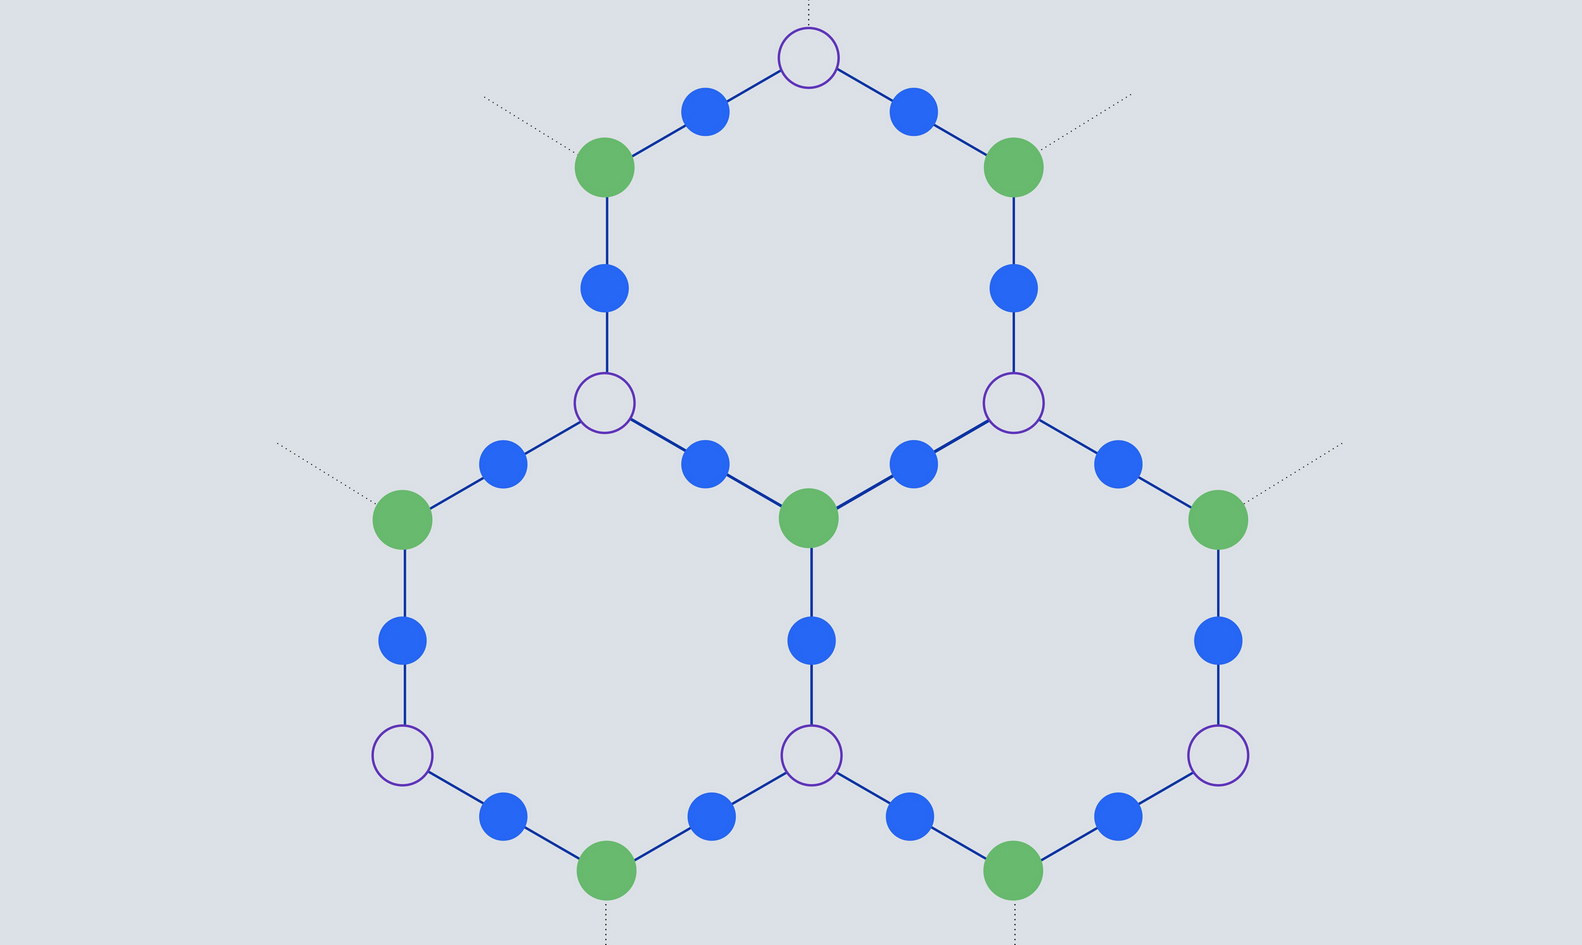
\includegraphics[width=0.5\linewidth]{Figuras/Fig_scq_hhl.png}
	\caption{Topología ``heavy hex lattice''}
	\label{Fig_scq_hhl}
	\end{figure}


	\begin{figure}[H]
	\centering 
	\includegraphics[width=1\linewidth]{Figuras/Fig_scq_topologías_IBM.png}
	\caption{Topología de red de diferentes chips de IBM donde se puede apreciar el uso de la conectividad ``heavy hex lattice''. }
	\label{Fig_scq_topologías_IBM}
	\end{figure}


Un nuevo enfoque consiste en utilizar chipsets de conectividad de múltiples capas que se conectan al chipset de qubits con conectores verticales TSV (through-silicon vias). Los diseños más recientes de IBM y los laboratorios Lincoln del MIT tienen entre tres y siete capas metálicas. 

	\begin{figure}[H]
	\centering 
	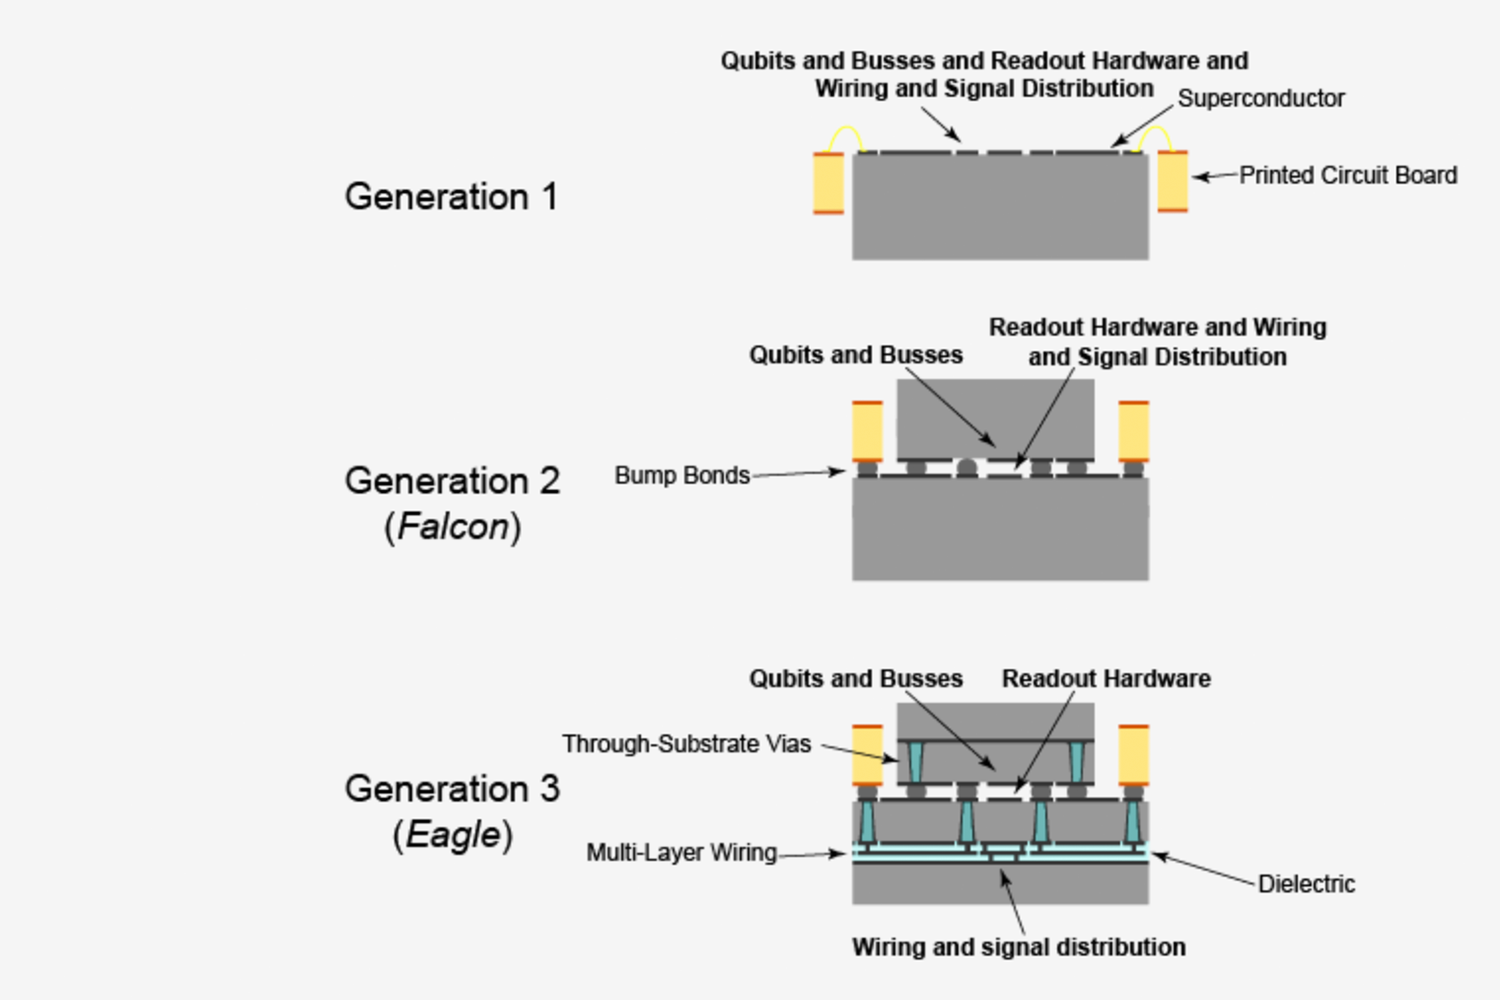
\includegraphics[width=1\linewidth]{Figuras/Fig_scq_MLW.png}
	\caption{Arquitecturas con una, dos y varias capas de chips de IBM.}
	\label{Fig_scq_MLW}
	\end{figure}

\begin{mybox_blue}{Nota: Los proceadores Falcon y Humminbird de IBM}
IBM utilizó por primera vez este tipo de arquitectura multicapa en el procesador \textbf{Eagle} de 127 qubits (ver Fig \ref{Fig_scq_eagle_127}).  Para el procesador Eagle, como antes, se usó una oblea de qubits unida a una oblea intercalada. Sin embargo, en este procesador se añadió un \textbf{cableado multicapa} (\textbf{MLW}, de sus siglas en inglés) dentro del intercalador. Las señales de control y lectura se dirigen en esta capa adicional, que está bien aislada del propio dispositivo cuántico y permite enviar señales a gran profundidad en chips de gran tamaño.  El nivel MLW consta de tres capas metálicas, un dieléctrico planarizado entre cada nivel y unas conexiones cortas llamadas vías que conectan los niveles metálicos. Juntos, estos niveles permiten crear líneas de transmisión totalmente aisladas entre sí y del dispositivo cuántico. También se añadieron vías a través del sustrato a los chips de qubits e intercalador.
\end{mybox_blue}

	\begin{figure}[t]
	\centering 
	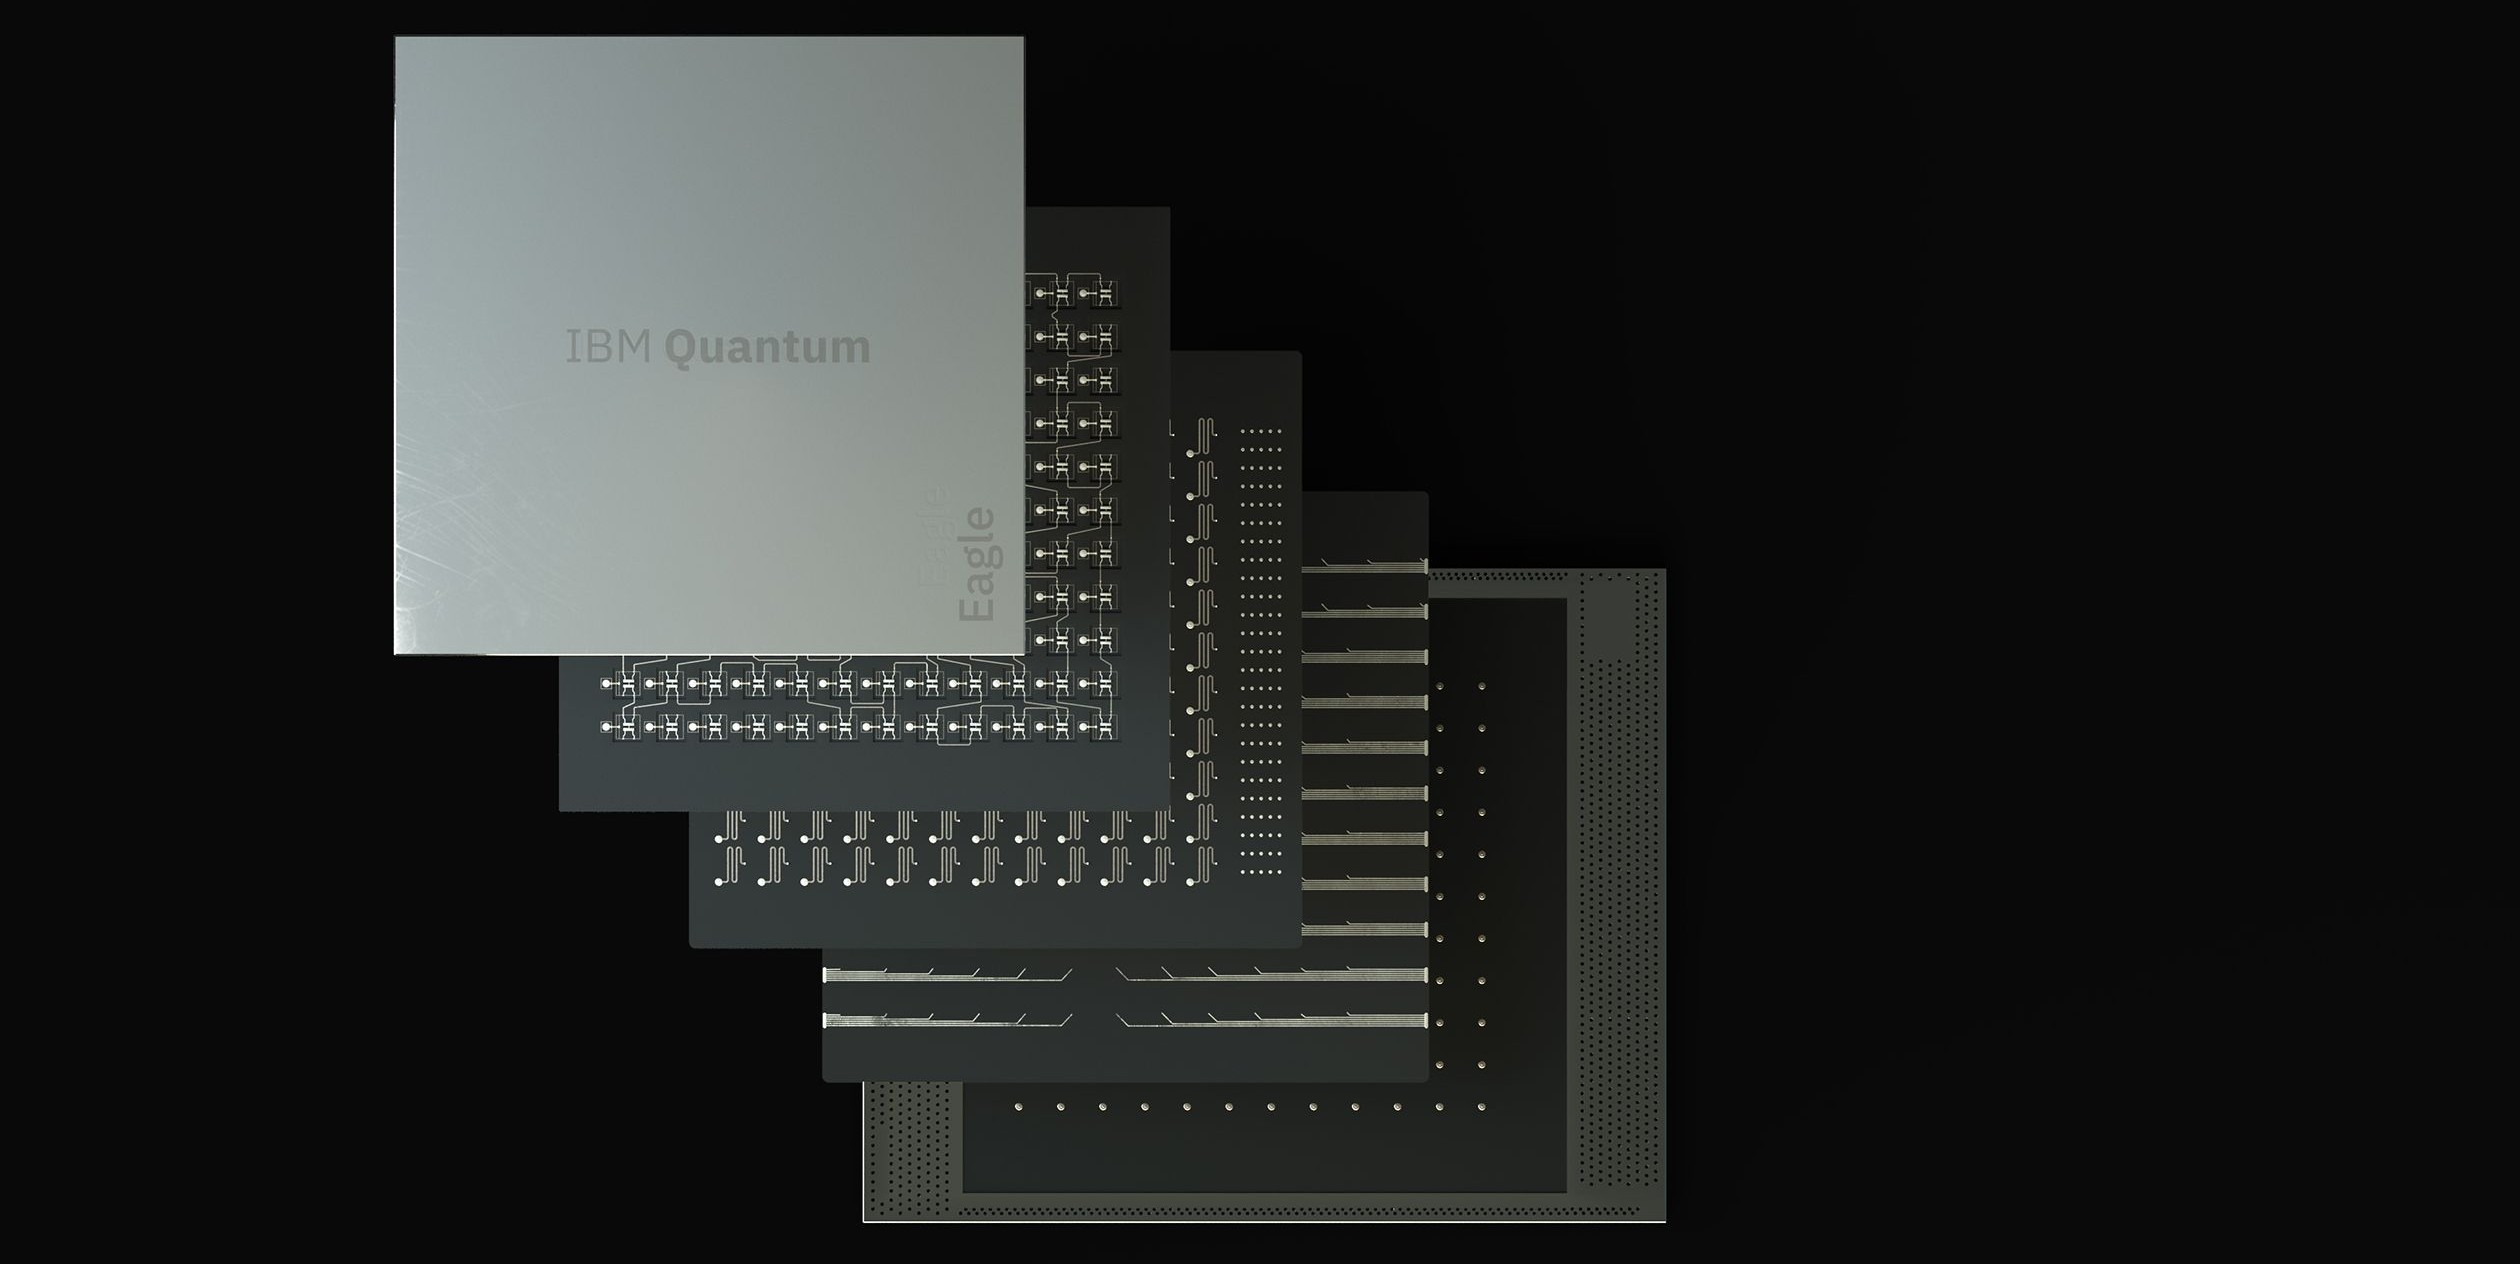
\includegraphics[width=1\linewidth]{Figuras/Fig_scq_eagle_127.jpeg}
	\caption{Procesador Eagle de 127 qubits de IBM}
	\label{Fig_scq_eagle_127}
	\end{figure}



\section{Retos con qubits superconductores}

Como todos los tipos de qubits, los superconductores tienen sus dificultades para permitir la creación de ordenadores cuánticos útiles, ya sea en el ámbito NISQ o FTQC. Sobre el papel, la tecnología podría ampliarse a miles, si no millones, de qubits. Las mejores fidelidades de su clase las obtuvo IBM con su procesador Egret de 33 qubits en noviembre de 2022, con una fidelidad de puerta de dos qubits del 99,7\%. Crear un ordenador cuántico tolerante a fallos requeriría al menos unos 100.000 qubits físicos con una fidelidad del 99,9\%. Esto permitiría 100 qubits lógicos y una profundidad de cálculo equivalente. 

En este punto se plantean las siguientes cuestiones:
\begin{itemize}
\item ¿puede contenerse la interferencia entre qubits a esta escala? 
\item ¿Es posible entrelazar de forma controlada sistemas cuánticos multicuerpo tan grandes? 
\item ¿Cómo diseñar códigos cuánticos de corrección de errores con una sobrecarga física de qubits y unos requisitos de fidelidad mínimos? 
\item ¿Es posible crear una electrónica de control de bajo consumo, cableado, multiplexación y criogenia adecuados para alcanzar tal escala?
\item ¿Será posible interconectar varios procesadores cuánticos con microondas o recursos de fotones entrelazados? 
\end{itemize}
Todos estos y más retos científicos y tecnológicos son gigantescos.

Mientras tanto, proveedores como IBM, Rigetti y Google intentan crear sistemas NISQ con cientos de qubits que podrían aportar alguna ventaja a la computación cuántica gracias a la técnica de mitigación de errores cuánticos que funciona con algoritmos de poca profundidad, en particular los \textbf{algoritmos variacionales} que trabajan en modo híbrido junto con superordenadores. La creación de sistemas NISQ utilizables seguiría requiriendo fidelidades de puerta muy superiores a las disponibles en la actualidad, con fidelidades de puerta de dos qubits superiores al 99.99\%.









\chapter{Técnicas de control y computación en RMN.}

En este capítulo vamos a ver un poco más en detalla como se implementa un computador cuántico. En concreto, veremos de manera relativamente profunda el formalismo detrás del control de los qubits en \textbf{RMN} (Resonancia Magnética Nuclear). Esto es debido a que, a pesar de que actualmente las implementaciones de los qubits son variopintas, la teoría detrás del control de los qubits es más o menos igual. 

	\section{Introducción.}

El problema del control de sistemas cuánticos acoplados múltiples es un tema emblemático de la RMN, y puede resumirse como sigue: dado un sistema con Hamiltoniano
\begin{equation}
\mathcal{H} = \mathcal{H}_{sys} + \mathcal{H}_{control}
\end{equation}
donde $\mathcal{H}_{sys}$ es el Hamiltoniano del sistema en ausencia de cualquier control, y $\mathcal{H}_{control}$ describe términos que están bajo control externo, ¿cómo puede aplicarse una transformación unitaria $U$ deseada, en presencia de imperfecciones y utilizando un mínimo de recursos? De forma similar a otros escenarios en los que el control cuántico es una idea bien desarrollada, como en la excitación láser de reacciones químicas, $\mathcal{H}_{control}$ \textbf{surge de secuencias sincronizadas con precisión de múltiples pulsos de radiación electromagnética, aplicados de forma coherente en fase, con diferentes anchuras, frecuencias, fases y amplitudes de pulso.}

En RMN lo que se controla con esto pulsos es el \textbf{espín nuclear}. Tenemos que ver entonces que es el espín nuclear (sección \ref{sec_sub_Harware_NMR_espin}), como se puede usar para formar qubits (construir $\mathcal{H}_{sys}$, sección \ref{sec_subsub_Harware_NMR_H_sys}) y como se  manipulan usando pulsos electromagnéticos (construir $\mathcal{H}_{control}$, sección \ref{sec_subsub_Harware_NMR_H_control}). Finalmente, veremos más en detalle como se implementan estos pulsos (sección \ref{sec_sub_Harware_NMR_pulsos}).

Para más información en general sobre física núclear, puede consultarse un libro clásico como es \cite{bib_Krane:359790}. Para más información sobre como controlar qubits de RMN puede consultarse \cite{bib_NMR_hardware}. Gran parte de este capítulo se basa en intentar explicar de una forma más simple este último artículo.



		\section{El espín nuclear} \label{sec_sub_Harware_NMR_espin}

En el núcleo, cada nucleón (protones o neutrones) posee un momento angular orbital y un momento angular intrínseco o espín. Al igual que el electrón, los nucleones son fermiones de espín $\hbar/2$. 

A cada \textbf{estado nuclear} se asigna un único número cuántico de espín $I$, representando el \textbf{momento angular total} (orbital más intrínseco) de todos los nucleones en el núcleo. El vector $\vec{I}$ puede considerarse como la suma de las contribuciones orbital y intrínseca (espín intrínseco de protones y neutrones) de los momento angulares de los nucleones
\begin{equation} \label{ec_Hardware_NMR_I}
\begin{aligned} 
\vec{I} ~ & =  ~ \, \sum_{i=1}^A (\vec{l_i} +  \vec{s_i}) \nonumber \\
& = ~ \,  \vec{L} + \vec{S}  \\
& = ~ \, \sum_{i=1}^A \vec{j_i} \nonumber
\end{aligned}
\end{equation}
donde $A$ es el \textbf{número másico} 
	\begin{equation}
	A = Z + N 
	\end{equation}
donde $Z$ es el \textbf{número de protones} y $N$ el \textbf{número de neutrones}.

El \textit{número cuántico} $I$ tiene la conexión  usual con el \textit{vector} $\vec{I}$:
\begin{equation} 
\begin{aligned}
| \vec{I} | ~ = & ~\,  \sqrt{I(I+1)} \hbar \\
I_i ~ = & ~\, m_i \hbar \qquad (m_i = I, I-1, \dots, -I +1, -I)
\end{aligned}
\end{equation}
Al vector $\vec{I}$ se lo denomina \textbf{espín nuclear}.

	\begin{mybox_blue}{Nota: $S_z$ e $I_Z$}
	Aunque aquí hayamos decidido usar una notación difenciadora para el spín de una partícula 
	y un núcleo ($\vec{S}$ y $\vec{I}$), a partir de aquí \textbf{usaremos $\vec{S}$ para todo}.
	\end{mybox_blue}



	\begin{mybox_blue}{Nota: Operador de espín para partículas de espín 1/2}
	En física cuántica todos los observables son operadores (matrices hermíticas). Ya hemos visto 
	el vector de espín, $\vec{S}$ (o $\vec{I}$, pero ya comentamos que abandonamos esta notación),
	ahora nos falta ver el \textbf{operador espín},	$\hat{S}$ o simplemente $S$. Para partículas de 
	espín 1/2, este toma la forma
		\begin{equation} \label{ec_Hardware_NMR_operador_S_sigma_vec}
		\boxed{S = \frac{\hbar}{2} \vec{\sigma}}
		\end{equation}
	donde $\vec{\sigma}$ es el vector de matrices de Pauli $(\sigma_x, \sigma_y, \sigma_z)$.
	También podemos escribirlo pues como
		\begin{equation} \label{ec_Hardware_NMR_operador_S_vec_Sx-Sy-Sz}
		S = (S_x, S_y, S_z)
		\end{equation}
	donde 
		\begin{equation} \label{ec_Hardware_NMR_Sx-Sy-Sz}
		\boxed{S_x = \frac{\hbar}{2} \sigma_x} \, , \hspace{2cm} 
		\boxed{S_y = \frac{\hbar}{2} \sigma_y} \, , \hspace{2cm} 
		\boxed{S_z = \frac{\hbar}{2} \sigma_z} \, .
		\end{equation}
	\end{mybox_blue}
	
	\begin{mybox_blue}{Nota: Operador momento angular}
	Es común en física que se usen la notación $I = (I_x, I_y, I_z)$ para hablar del 
	\textbf{operador de momento angular}. No confundirlo con el espín nuclear que vimos
	antes. Este operador es simplemente el operador de espín (\ref{ec_Hardware_NMR_operador_S_sigma_vec})
	pero sin el factor $\hbar$, es decir,
		\begin{equation} 
		I = \frac{1}{2} \vec{\sigma}
		\end{equation}
	Por ejemplo, en el paper de referencia de esta sección \cite{bib_NMR_hardware} se usa esta notación. 
	\end{mybox_blue}

La Ec. (\ref{ec_Hardware_NMR_I}) representa lo que en principio podría ser un acoplamiento muy complicado de muchos vectores para dar un solo resultado, y puede que no sea evidente por qué podemos despreciar esta estructura interna y tratar el núcleo como si fuera un momento angular una ``partícula''. Esto es posible porque las interacciones a las que sometemos el núcleo, como los campos electromagnéticos, no son suficientemente fuertes como para cambiar la estructura interna o romper los acoplamientos de los nucleones que son responsables de la Ec. (\ref{ec_Hardware_NMR_I}). 

El valor del espín nuclear depende del valor del número másico:
\begin{align*}
& \text{Núcleos con }A \text{ impar:} ~ \longrightarrow \text{Espín nuclear, } I \text{, semientero}   \\
& \text{Núcleos con }A \text{ par:} ~~~ \,\, \, \longrightarrow \text{Espín nuclear, } I \text{, entero}
\end{align*}
Esto es debido a que los nucleones tienden a acoplarse en parejas de iguales (pp y nn) con el mismo momento angular orbital pero con los espines opuestos, situación consistente con el principio de exclusión de Pauli y que minimiza la energía potencial del sistema permitiendo un mayor solapamiento de las funciones de onda de los nucleones. Teniendo esto en cuenta, es de esperar que usualmente las propiedades magnéticas nucleares estén determinadas por el último nucleón desapareado (si existe), por el acoplamiento de la última pareja de nucleones, ó por el acoplamiento del espín del nucleón desapareado con el espín del core nuclear residual (bastante similar a lo que ocurre con los electrones más externos de los átomos).

Todos los núcleos que se conocen (estables e inestables) con $Z$ par y $N$ par tienen espín cero en el estado fundamental. Lo cual es una evidencia de que la interacción fuerte manifiesta una especie de fuerza de apareamiento tal que existe una tendencia a mantener los nucleones apareados. Como consecuencia, resulta que el espín del estado fundamental de un núcleo con $A$ impar debe ser igual al $\vec{j_i} = \vec{s_i} + \vec{l_i}$ del protón o neutrón desapareado.


	
	\section{qubits de RMN} 

En esta sección vamos a describir como es el sistema con el que se construyen los qubits en RNM, basándonos en su \textbf{Hamiltoniano del sistema} y su \textbf{Hamiltoniano de control}. El Hamiltoniano del sistema da la energía de los espines simples y acoplados en un campo magnético estático, y el Hamiltoniano de control surge de la aplicación de pulsos de radiofrecuencia al sistema en, o cerca de, sus frecuencias resonantes. Veremos que para describir el efecto de los pulsos es más conveniente usar un \textbf{sistema de referencia giratorio}.


		\subsection{Hamiltoniano del sistema} \label{sec_subsub_Harware_NMR_H_sys}


			\SubsubiIt{Espines simples.} 

Una partícula con espín constituye un \textbf{dipolo magnético}. En esencia, dipolo magnético es un pequeño imán, es decir, una fuente de campo magnético. El \textbf{momento dipolar magnético}, $\vec{\mu}$, es proporcional al momento angular de espín, $\vec{S}$:
	\begin{equation} \label{ec_Hardware_NMR_mu}
	\vec{\mu} = \gamma \vec{S}\, ,
	\end{equation}
donde la constate de proporcionalidad, $\gamma$, se denomina ratio giromagnético (\textbf{gyromagnetic ratio}). Este toma la forma
	\begin{equation} \label{ec_Hardware_NMR_gamma}
	\gamma = g \frac{q}{2m} \, ,
	\end{equation}
donde $q$ es la carga eléctrica de la partícula, $m$ su masa y $g$ se denomina \textbf{factor $g$ ($g$-factor)}. 

Cuando un dipolo magnético se sitúa en un campo magnético $\vec{B}$, este dipolo experimenta un torque, $\vec{\mu} \times \vec{B}$, que tiende a alinearlo paralelo al campo (como la aguja de una brújula). La energía asociada con este torque es
	\begin{equation}
		E = - \vec{\mu} \cdot \vec{B}
		\end{equation}	
con lo que el Hamiltoniano para una partícula cargada con espín, en reposo en un campo magnético $\vec{B}$, es
	\begin{equation}
	\mathcal{H} = - \gamma \vec{B} \cdot S
	\end{equation}
donde $S$ es el operador de espín (ver Ec. (\ref{ec_Hardware_NMR_operador_S_sigma_vec}) para el caso de partículad de espín 1/2).

Si tenemos una partícula (o un núcleo) de espín 1/2 (no consideraremos espines de mayor orden en estas notas) en un campo magnético $\vec{B}_0$ a lo largo del eje $\hat{z}$, entonces su evolución temporal está gobernada por el Hamiltoniano
	\begin{equation} \label{ec_Hardware_NMR_H_sys_1}
	\boxed{\mathcal{H} = -  \gamma B_0 S_z = - \omega_0 S_z = 
	\begin{bmatrix}
	- \hbar \omega_0/2  & 0 \\
	0  &  \hbar \omega_0 /2
	\end{bmatrix}} \, ,
	\end{equation}
donde 
\begin{itemize}
	\item $\gamma$ es ratio giromagnético del núcleo (ver Ec. (\ref{ec_Hardware_NMR_gamma})),
	\item $\omega/2 \pi = \gamma B_0 $ es la \textbf{frecuencia de Larmor}
	\item e $S_z$ es el operador de espín en la dirección $\hat{z}$ (ver Ec. (\ref{ec_Hardware_NMR_Sx-Sy-Sz})).
\end{itemize}

\begin{mybox_blue}{Nota: frecuencia y frecuencia angular}
En Física, la \textbf{frecuencia} se define como el inverso del periodo de rotación: $f = 1/T$ y se mide en Hz (1/segundos). Además, se define la \textbf{frecuencia angular} como $\omega = 2\pi f$ y se mide en radianes/segundo. Muchas veces se denomina a las dos, simplemente, frecuencia.
\end{mybox_blue}

La interpretación de la Ec. (\ref{ec_Hardware_NMR_H_sys_1}) es simple. Cuando tenemos una partícula de espín 1/2 aislada, las dos proyecciones del espín son \textbf{degeneradas}, es decir, tiene la misma energía. Esto es fácil de entender si pensamos en que no hay ninguna dirección privilegiada en el sistema. Cuando introducimos un campo magnético, ahora sí hay una dirección privilegiada: aquella con el momento dipolar magnético $\vec{\mu}$ apuntando en la misma dirección que el campo magnético. Esto es debido a que el espín es como un pequeño imán y tiende a orientarse con el campo magnéticos. En este momento, el sistema pasa a ser \textbf{no-degenerado}, y un estado tiene más energía que el otro.

Esto último se traduce matemáticamente en la Ec. (\ref{ec_Hardware_NMR_H_sys_1}). Como el Hamiltoniano es diagonal, los elementos de la diagonal son las energías de los estados. Vemos que el estado con el espín apuntando en la misma dirección (es estado $\ket{0}$ o $\ket{\uparrow}$) que el campo magnético tiene menos energía que el estado que apunta en la dirección contraria (el estado $\ket{1}$ o $\ket{\downarrow}$). La diferencia de energía entre los estados es de $\hbar \omega_0$, como se puede ver en la Fig. \ref{Fig_Harware_NMR_split_Zeeman}. Esta separación de energías (\textit{energy splitting}) se conoce como \textbf{Zeeman spliting}.

	\begin{figure}[H]
	\centering 
	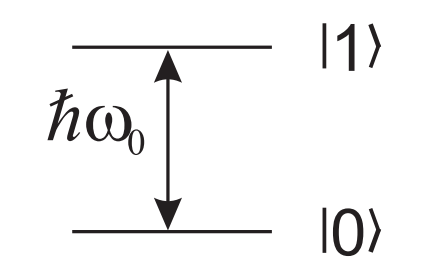
\includegraphics[width=0.15\linewidth]{Figuras/Fig_Harware_NMR_split_Zeeman.png}
	\caption{Diagrama de energías de una partícula de espín 1/2 en un campo magnético.}
	\label{Fig_Harware_NMR_split_Zeeman}
	\end{figure}


Podemos entender gráficamente la evolución temporal $U = e^{-i \mathcal{H} t/ \hbar}$ bajo el Hamiltoniano de la Ec. (\ref{ec_Hardware_NMR_H_sys_1}) como un movimiento de precesión en la esfera de Bloch al rededor de $\vec{B}_0$, como se muestra en la Fig. \ref{Fig_Harware_NMR_precesion}. Como es habitual, definimos el eje $\hat{z}$ de la esfera de Bloch como el eje de cuantización del Hamiltoniano, con $\ket{0}$ a lo largo de $+\hat{z}$ y $\ket{1}$ a lo largo de $-\hat{z}$.

	\begin{figure}[H]
	\centering 
	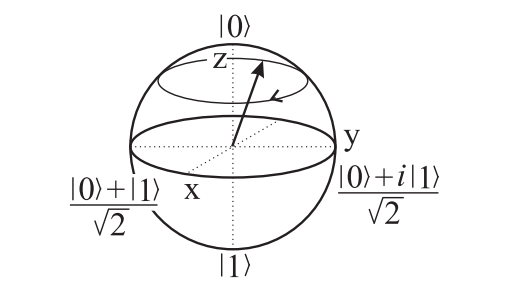
\includegraphics[width=0.45\linewidth]{Figuras/Fig_Harware_NMR_precesion.png}
	\caption{Precesión del valor esperado del espín entorno al campo magnético.}
	\label{Fig_Harware_NMR_precesion}
	\end{figure}

	\begin{mybox_blue}{Nota: Esfera de Bloch para el espín}
	Véase que para el espín la representación en la esfera de Bloch no es más que la representación 
	en 3D del vector de espín. 	
	\end{mybox_blue}

	\begin{mybox_blue}{Nota: orientación del espín}
	En las Ecs. (\ref{ec_Hardware_NMR_mu}) y (\ref{ec_Hardware_NMR_gamma}) vemos que el vector de espín
	y el momento dipolar magnético se relacionan por una constate que $\gamma$ que puede ser positiva o 
	negativa, dependiendo del valor de la carga eléctrica de la partícula. Es decir, estos vectores pueden 
	apuntar en la misma dirección o en dirección opuesta. 

	\vspace{0.3cm}	
	Hemos comentado que cuando tenemos un campo magnético, el
	estado de menor energía es aquel con el \textbf{momento dipolar magnético} apuntando en la dirección 
	del campo. Como podemos ver en la Fig. \ref{Fig_Hardware_NMR_espines_en_B}, tenemos dos opciones 
	dependiendo de la carga de la partícula.
		\begin{figure}[H]
		\centering 
		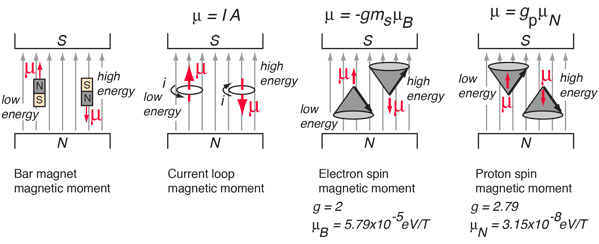
\includegraphics[width=1\linewidth]{Figuras/Fig_Hardware_NMR_espines_en_B.png}
		\caption{Momentos dipolares magnéticos en presencia de un campo magnético externo. En las dos figuras de la derecha vemos que, dependiendo de la carga de la partícula, el momento dipolar puede apuntar en la misma dirección o en la contraria al espín. Figura tomada de \url{http://hyperphysics.phy-astr.gsu.edu/hbase/Nuclear/nmr.html}}
		\label{Fig_Hardware_NMR_espines_en_B}
		\end{figure}
	\end{mybox_blue}


Vemos a la demostración de que el valor esperado del espín precesa entorno al campo magnético:

\begin{proof}
\textbf{(Precesión de Larmor, Griffiths \cite{bib_griffiths_schroeter_2018} ejemplo 4.3)} 

Supongamos una partícula con espín 1/2 sometida a un campo magnético en la dirección $\vec{z}$, i.e. $\vec{B}_0 = B_0 \hat{z}$. El Hamiltoniano estará dado por 
	\begin{equation}
	\mathcal{H} = - \gamma B_0 S_z = - \frac{\gamma B_0 \hbar}{2} 
	\begin{bmatrix}	1 & 0 \\ 0 & -1 \end{bmatrix}
	\end{equation}
Los autovectores y autovalores (energías) de este Hamiltoniano son
	\begin{equation}
	\lch 
	\begin{matrix}
	\ket{0} = \begin{bmatrix} 1 \\ 0 \end{bmatrix} \, 
	\text{con energía } E_{\ket{0}} = - (\gamma B_0 \hbar) /2 \, \\
	\ket{1} = \begin{bmatrix} 0 \\ 1 \end{bmatrix} \, 
	\text{con energía } E_{\ket{1}} = + (\gamma B_0 \hbar) / 2
	\end{matrix}
	\right.
	\end{equation}
La energía es menor cando el momento dipolar es paralelo al campo magnético, al igual que en el caso clásico.

Como el Hamiltoniano es independiente del tiempo, la solución general para la ecuación de Schrödinger dependiente de tiempo,
	\begin{equation} \label{ec_Hardware_NMR_schrodinger}
	i \hbar \frac{\partial \ket{\Psi}}{\partial t} = \mathcal{H} \ket{\Psi}
	\end{equation}
puede expresarse en función de estados estacionarios:
	\begin{equation} \label{ec_Hardware_NMR_schrodinger_sol}
	\ket{\Psi (t)} = a  e^{-i E_{\ket{0}} t/ \hbar} \ket{0} + b  e^{-i E_{\ket{1}} t/ \hbar} \ket{1}  =
	\begin{bmatrix}
	a e ^{i \gamma B_0 t/2} \\
	b e ^{i \gamma B_0 t/2}
	\end{bmatrix}
	\end{equation}

Las constantes $a$ y $b$ se pueden determinar mediante las condiciones iniciales:
	\begin{equation}
	\ket{\Psi (t = 0)} = \begin{bmatrix} a \\ b	\end{bmatrix}
	\end{equation}
(por supuesto, $|a|^2 + |b|^2 = 1$). Sin perdida de generalidad, podemos elegir $a = \cos (\alpha/2)$ y $b = \sin (\alpha/2)$, donde $\alpha$ es un ángulo fijo cuyo significado físico veremos dentro de poco.
Tenemos entonces
	\begin{equation}
	\ket{\Psi (t)} = 
	\begin{bmatrix} 
	\cos (\alpha/2) e^{i \gamma B_0 t/2} \\ 
	\sin (\alpha/2) e^{-i \gamma B_0 t/2} 
	\end{bmatrix}
	\end{equation}
Para ver que está pasando con el espín bajo la evolución de este Hamiltoniano, calculemos el calor esperado del espín $\vec{S}$ como función del tiempo.
	\begin{equation} 
\begin{aligned}
	\left\langle S_x \right\rangle = & \, \bra{\Psi(t)} S_x \ket{\Psi(t)} = 
	\nonumber \\
	= & \, \Lc \psi_0^* \quad \psi_1^* \Rc 
	\begin{bmatrix} 1 & 0 \\ 0 & 1 \end{bmatrix}  
	\begin{bmatrix} \psi_0 \\ \psi_1 \end{bmatrix} 
	\nonumber \\
	= & \, \Lc a e ^{-i \gamma B_0 t/2} \qquad  b e ^{-i \gamma B_0 t/2} \Rc 
	\frac{\hbar}{2} \begin{bmatrix} 0 & 1 \\ 1 & 0 \end{bmatrix} 
	\begin{bmatrix} \cos (\alpha/2) e^{i \gamma B_0 t/2} \\ \sin (\alpha/2) e^{-i \gamma B_0 t/2} \end{bmatrix} 
	\nonumber \\
	= & \, \frac{\hbar}{2} \sin \alpha \cos (\gamma B_0 t ) 
	\end{aligned}
\end{equation}
De forma análoga,
	\begin{equation} 
\begin{aligned}
	\left\langle S_y \right\rangle = & \, - \frac{\hbar}{2} \sin \alpha \sin (\gamma B_0 t )  \\
	\left\langle S_z \right\rangle = & \frac{\hbar}{2} \cos \alpha
	\end{aligned}
\end{equation}

Con lo cual, $\left\langle \vec{S} \right\rangle$ está inclinado un ángulo $\alpha$ respecto al eje $\hat{z}$, y precesa al rededor del campo con una frecuencia 
	\begin{equation}
	f_0 = \omega_0 / 2 \pi = \gamma B_0 / 2 \pi
	\end{equation}
(la frecuencia de Larmor) al igual que en el caso clásico (una peonza inclinada). No tenemos ninguna sorpresa aquí, pues el teorema de Ehrenfest nos asegura que los valores esperados evolucionan de acuerdo a las leyes clásicas del movimiento (algunos autores limitan esta afirmación solo al par de ecuaciones $\left\langle p \right\rangle = m d \left\langle x \right\rangle / dt$ y $\left\langle - \partial V / \partial x \right\rangle = d \left\langle p \right\rangle / dt$) Puede verse esto en el Griffiths, \cite{bib_griffiths_schroeter_2018}. 
	\begin{figure}[H]
	\centering 
	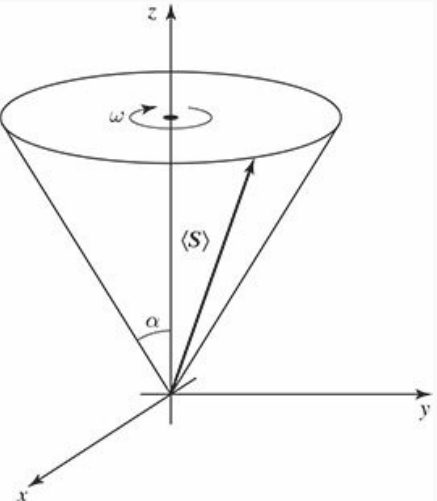
\includegraphics[width=0.30\linewidth]{Figuras/Fig_Harware_NMR_precession_griffiths.png}
	\caption{Precesión de Larmor en un campo magnético uniforme.}
	\label{Fig_Harware_NMR_precession_griffiths}
	\end{figure}

\end{proof}


	\Ejercicio{
	Verifica que la Ec. (\ref{ec_Hardware_NMR_schrodinger_sol}) es solución de la ecuación de Schrödinger, Ec. (\ref{ec_Hardware_NMR_schrodinger})
	}

El Hamiltoniano de espín para una molécula con $n$ núcleos desacoplados viene dado por 
	\begin{equation} \label{ec_Hardware_NMR_H_single}
	\mathcal{H}_0 = - \sum_{i=1}^n  \omega_0^i S_z^i
	\end{equation}
Véase que, los espines de especies nucleares diferentes (espines heteronucleares) tendrán diferentes valores de $\omega_0^i$, así como también es posibles que los espines de la misma especie nuclear (espines homonucleares) que formen una molécula  tengan también diferentes valores de esta frecuencia.


			\SubsubiIt{Espines que interactúan.} 

Para espines nucleares en moléculas, la naturaleza nos proporciona dos mecanismos de interacción diferentes que vamos a describir: 
\begin{itemize}
	\item \textbf{Interacción directa dipolo-dipolo.}
	
La interacción magnética dipolo-dipolo es similar a la interacción entre dos barras magnéticas cercanas. Tiene lugar puramente a través del espacio (no se requiere ningún medio para esta interacción) y depende del vector internuclear $\vec{r}_{ij}$ que conecta los dos núcleos $i$ y $j$, tal y como describe el Hamiltoniano
	\begin{equation} \label{ec_Hardware_NMR_H_dipolo-dipolo}
	\mathcal{H}_D = \sum_{i<j} \frac{\mu_0 \gamma_i \gamma_j}{4 \pi | \vec{r}_{ij}|^3 \hbar} 
	\lc \vec{S}^i \cdot \vec{S}^j - \frac{3}{| \vec{r}_{ij}|^2} \lp \vec{S}^i \cdot \vec{r}_{ij} \rp \lp \vec{S}^j \cdot \vec{r}_{ij} \rp \rc
	\end{equation}
donde $\mu_0$ es la permeabilidad magnética habitual del espacio libre. 

No vamos a entrar en dalles sobre esta interacción, pues usualmente se promedia y no tiene efecto.
	
	\item \textbf{Interacción del contrato de Fermi mediada por electrones (acoplamiento J).}

	El segundo mecanismo de interacción entre los espines nucleares de una molécula es el acoplamiento $J$ o acoplamiento escalar. Esta interacción está mediada por los electrones compartidos en los enlaces químicos entre los átomos, y es debido al solapamiento de la función de onda del electrón compartido con los dos núcleos acoplados. Es decir, una interacción de contacto de Fermi. La fuerza de acoplamiento de enlace J depende de la especie nuclear respectiva y disminuye con el número de enlaces químicos que separan los núcleos.

El Hamiltoniano es
	\begin{equation}
	\mathcal{H} = \frac{1}{\hbar} \sum_{i <j} 2 \pi J_{ij} S^i S^j = 
	\frac{1}{\hbar} \sum_{i < j} 2 \pi J_{ij} \lp S_x^i S_x^j + S_y^i S_y^j + S_z^i S_z^j  \rp
	\end{equation}
donde $J_{ij}$ es la fuerza de acoplamiento entre los espines $i$ y $j$. Cuando $| \omega_0^i - \omega_0^j |$ es mucho más grande que el acoplamiento $J_{ij}$ ($| \omega_0^i - \omega_0^j | \gg 2 \pi |J_{ij}|$), los acoplamiento transversos se pueden despreciar. De esta forma, el Hamiltoniano se simplifica
	\begin{equation} \label{ec_Hardware_NMR_J_coupling}
	\boxed{\mathcal{H}_j = \frac{1}{\hbar} \sum_{i < j}^n 2 \pi J_{ij} S_z^{i} S_z^{j}}
	\end{equation}
Esta condición ($| \omega_0^i - \omega_0^j | \gg 2 \pi |J_{ij}|$) se cumple fácilmente para los espines heteronucleares y que también puede cumplirse para las moléculas homonucleares pequeñas.

La interpretación del término de acoplamiento escalar de la Ec. (\ref{ec_Hardware_NMR_J_coupling})\textit{ es que un espín ``siente'' un campo magnético estático a lo largo de $\pm z$ producido por los espines vecinos}, además del campo $\vec{B}_0$ aplicado externamente. Este campo adicional desplaza los niveles de energía como podemos ver en la Fig. \ref{Fig_Harware_NMR_diagrama}. Como resultado, la frecuencia de Larmor del espín $i$ se mueve en una cantidad $-J_{ij}/2$ si el espín $j$ está en el estado $\ket{0}$ (lineas rojas) y una cantidad $+J_{ij}/2$ si está en el estado $\ket{1}$ (líneas azules).  

	\begin{figure}[H]
	\centering 
	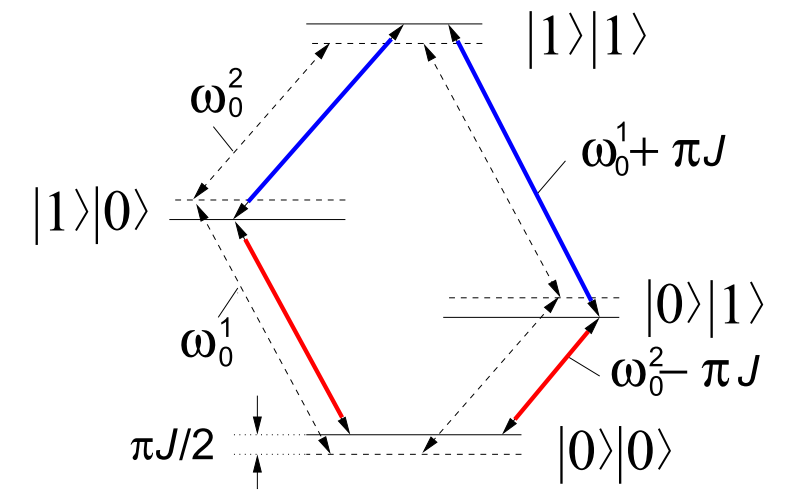
\includegraphics[width=0.4\linewidth]{Figuras/Fig_Harware_NMR_diagrama.png}
	\caption{Diagrama de niveles de energía para dos espines desacoplados (líneas discontinuas) y dos espines acoplados (líneas continuas) por un Hamiltoniano de la forma de la Ec.	(\ref{ec_Hardware_NMR_J_coupling}) (en unidades de $\hbar$). Marcadas en rojo están las dos transiciones en las que el espín que no cambia está en el estado $\ket{0}$, mientras que en azul están en las que el espín que no cambia está en el estado $\ket{1}$. Vemos que la energía de transición de las primera disminuye, mientras que de las segundas aumenta.}
	\label{Fig_Harware_NMR_diagrama}
	\end{figure}

\end{itemize}

			\SubsubiIt{Hamiltoniano completo.}

En resumen, la forma más simple del Hamiltoniano para un sistema de $n$ espines nucleares acoplados es, pues (de las Ecs. (\ref{ec_Hardware_NMR_H_single}) y (\ref{ec_Hardware_NMR_J_coupling}))
	\begin{equation} \label{ec_Hardware_NMR_H_sys_final}
	\boxed{\mathcal{H}_{sys} = - \sum_{i}^n \omega_0^i S_z^{i}  + \frac{1}{\hbar} \sum_{i<j} 2 \pi J_{ij} S_z^i S_z^j}
	\end{equation}
	

		\subsection{Hamiltoniano de control} \label{sec_subsub_Harware_NMR_H_control}

			\SubsubiIt{Campos de radiofrecuencia}

Pasemos ahora a los mecanismos físicos para controlar el sistema de RMN. El estado de una partícula de espín $1/2$ en un campo magnético estático $\vec{B}_0$ a lo largo del eje $\hat{z}$ puede manipularse aplicando un campo electromagnético $\vec{B}_1(t)$ que gira en el plano $\hat{x}-\hat{y}$ a frecuencia $\omega_{rf}$, en o cerca de la frecuencia de precesión del espín $\omega_0$. El Hamiltoniano de espín  correspondiente al campo de radiofrecuencia (RF) es, análogo a la Ec. (\ref{ec_Hardware_NMR_H_sys_1}) para el campo estático $B_0$,
	\begin{equation} 
	\mathcal{H}_{rf} = - \gamma B_1 \Lc \cos (\omega_{rf} + \phi) S_x + \sin (\omega_{rf} + \phi) S_y \Rc \,
	\end{equation}
donde $\phi$ es la fase del campo de RF, y $B_1$ su amplitud. Para $n$ espines tenemos
	\begin{equation} \label{ec_Hardware_NMR_H_rf}
	\boxed{\mathcal{H}_{rf} = - \sum_{i}^n \gamma_i B_1 \Lc \cos (\omega_{rf} t + \phi) S_x^i + \sin (\omega_{rf} t+ \phi ) S_y^i \Rc} \, ,
	\end{equation}
	
	\begin{mybox_blue}{Nota: implementación de un campo rotante en el laboratorio}
	En la práctica, se aplica un campo magnético que oscila a lo largo de un eje fijo en el
	laboratorio, perpendicular al campo magnético estático. Este campo oscilante puede
	descomponerse en dos campos contrarrotatorios, uno de los cuales gira a $\omega_{rf}$ en la
	misma dirección que el espín y, por tanto, puede establecerse en resonancia con el espín o
	cerca de ella. La  otra componente gira en la dirección opuesta y, por lo tanto, está muy 
	lejos de la resonancia (en aproximadamente $2\omega_0$). Como veremos, su único efecto es un
	desplazamiento insignificante de la frecuencia de Larmor, llamado desplazamiento Bloch-Siegert.
	\end{mybox_blue}

			\SubsubiIt{Sistema de referencia rotante (\textit{rotating frame}).} 
			
El movimiento de un espín nuclear individual sometido a un campo magnético estático y giratorio es bastante complejo cuando se describe en el sistema de coordenadas habitual del laboratorio (el marco del laboratorio). Sin embargo, se simplifica mucho describiendo el movimiento en un \textbf{sistema de coordenadas que gira} alrededor de $\hat{z}$ a frecuencia $\omega_{rf}$ (el \textbf{rotating frame}):
	\begin{equation} \label{ec_Hardware_NMR_psi_rot}
	\ket{\psi}^{rot} = \exp \lp -i \omega_{rf} t S_z/\hbar \rp \ket{\psi}
	\end{equation}
Para un solo espín libre, el Hamiltoniano será la suma (\ref{ec_Hardware_NMR_H_single}) y (\ref{ec_Hardware_NMR_H_rf}) (con $n=1$), es decir,
	\begin{equation} \label{ec_Hardware_NMR_H_lab_single}
	\mathcal{H} = - \omega_0 S_z - \omega_1 \Lc \cos (\omega_{rf} t+ \phi) S_x + \sin (\omega_{rf} t + \phi) S_y \Rc
	\end{equation}
Este Hamiltoniano junto con el estado en el sistema de referencia estático cumplen la ecuación de Schrödinger
	\begin{equation}
	i \hbar \frac{d \ket{\psi}}{dt} = \mathcal{H} \ket{\psi}
	\end{equation}
Sustituyendo el cambio de variable de la Ec. (\ref{ec_Hardware_NMR_H_sys_final}) en la ecuación de Schrödinger, podemos calcular como tendría que ser el $\mathcal{H}^{rot}$ que cumpla
	\begin{equation}
	i \hbar \frac{d \ket{\psi}^{rot}}{dt} = \mathcal{H}^{rot} \ket{\psi}^{rot}
	\end{equation}
Puede ver que el resultado es
	\begin{equation} \label{ec_Hardware_NMR_H_rot_single}
	\boxed{\mathcal{H}^{rot} = - (\omega_0 - \omega_{rf}) S_z - \omega_1 \Lc \cos (\phi) S_x + \sin  (\phi) S_y \Rc}
	\end{equation}

%\Ejercicio{Haz el cambio de variable comentado y calcula $\mathcal{H}^{rot}$ de la Ec. (\ref{ec_Hardware_NMR_H_rot_single})}

Naturalmente, el campo de RF se encuentra a lo largo de un eje fijo en el sistema de referencia que gira a $\omega_{rf}$. El movimiento del espín visto desde un sistema de referencia o el otro es diferente. 
\begin{itemize}
	\item En el \textbf{sistema laboratorio (en reposo)}, al aplicar el campo magnético rotante $\vec{B}_1$ lo que sucede es que \textit{el valor esperado del espín rota en espiral, bajando por la esfera}, como podemos ver en la Fig. \ref{Fig_Harware_NMR_espiral_bloch}b. 

	\begin{figure}[t]
	\centering 
	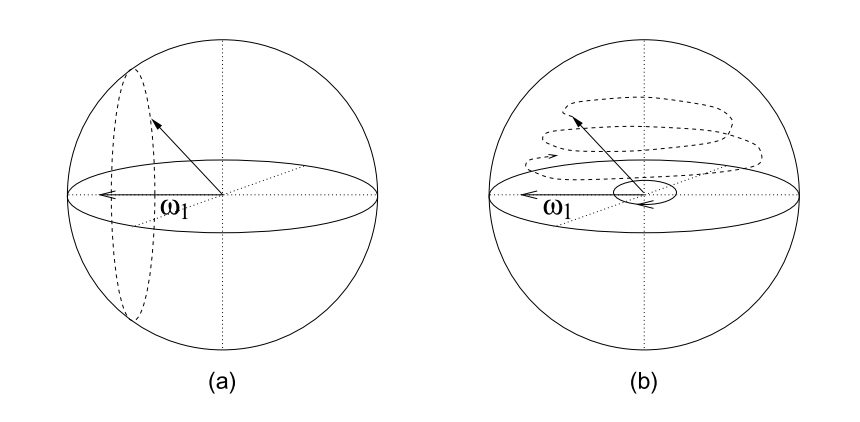
\includegraphics[width=0.55\linewidth]{Figuras/Fig_Harware_NMR_espiral_bloch.png}
	\caption{Nutación de un espín sometido a un campo de RF transversal observada en el marco de rotación (a) y observada en el marco de laboratorio (b).}
	\label{Fig_Harware_NMR_espiral_bloch}
	\end{figure}

	
	\item En el \textbf{sistema rotante}, tenemos dos casos:
	
	\begin{itemize}
		\item Caso \textbf{resonante} ($\omega_{rf} = \omega_0$): en este caso el primer término de la Ec. (\ref{ec_Hardware_NMR_H_rot_single}) desaparece. En este caso, un observador en el sistema rotante verá el espín simplemente \textit{precesar} alrededor de $\vec{B}_1$ (Fig. \ref{Fig_Harware_NMR_espiral_bloch}a), un movimiento llamado nutación. La elección de $\phi$ controla el eje de nutación.
		
		
		
		\item Caso \textbf{fuera de resonancia}: Si el campo de RF está fuera de resonancia con respecto a la frecuencia de espín en $\Delta \omega = \omega_0 - \omega_{rf}$, el espín precesa en el marco de rotación alrededor de un eje inclinado con respecto al eje $\vec{z}$ en un ángulo
	\begin{equation}
	\alpha = \arctan (\omega_1 / \Delta \omega)
	\end{equation}
como se ilustra en la Fig. \ref{Fig_Harware_NMR_nutacion_inclinada}.

	\begin{figure}[H]
	\centering 
	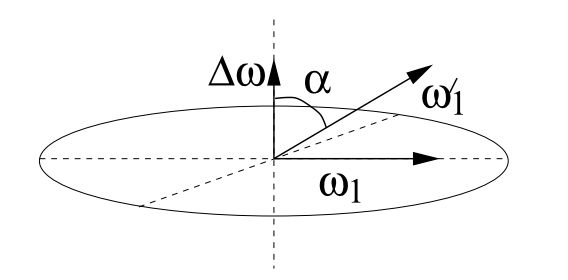
\includegraphics[width=0.35\linewidth]{Figuras/Fig_Harware_NMR_nutacion_inclinada.png}
	\caption{Eje de rotación (en el marco giratorio) durante un pulso de radiofrecuencia fuera de resonancia.}
	\label{Fig_Harware_NMR_nutacion_inclinada}
	\end{figure}
	
	\end{itemize}		

\end{itemize}

En este último caso se deduce que \textbf{el campo de RF no tiene prácticamente ningún efecto sobre espines que están lejos de la resonancia}, ya que $\alpha$ es muy pequeño cuando $|\Delta \omega | \gg \omega_1$ (ver Fig. \ref{Fig_Harware_NMR_espiral_bloch_2}). Si todos los espines tienen frecuencias de Larmor bien separadas, en principio podemos \textbf{rotar selectivamente} cualquier qubit sin rotar los otros espines.



Los pulsos moderadamente fuera de resonancia ($|\Delta \omega| \approx \omega_1$) hacen girar el espín, pero debido a la inclinación del eje de rotación, un solo pulso de este tipo no puede, por ejemplo, voltear un espín de $|0 \rangle$ a $|1 \rangle$ (véase de nuevo la Fig. \ref{Fig_Harware_NMR_espiral_bloch_2}). Por supuesto, los pulsos fuera de resonancia también pueden ser útiles, por ejemplo para la implementación directa de rotaciones sobre un eje fuera del plano $\hat{x} - \hat{y}$.

	\begin{figure}[H]
	\centering 
	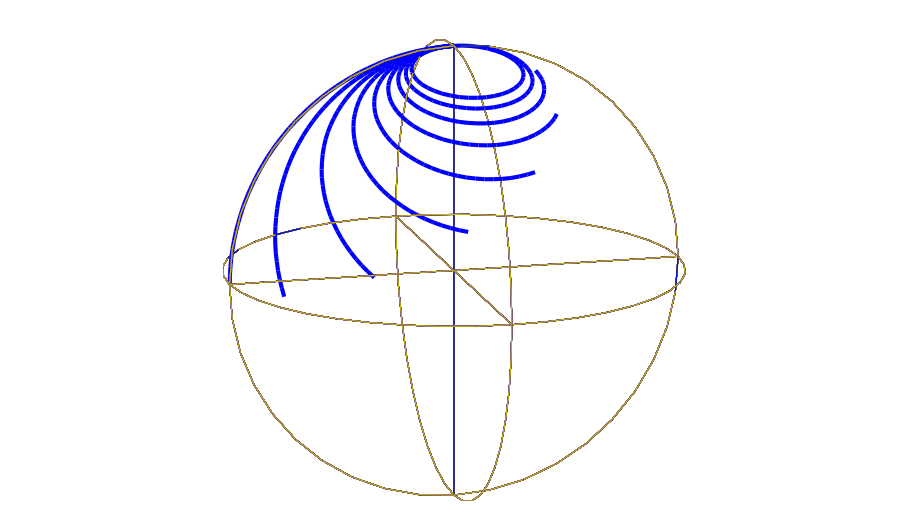
\includegraphics[width=0.4\linewidth]{Figuras/Fig_Harware_NMR_espiral_bloch_2.png}
	\caption{Trayectoria en la esfera de Bloch (en el sistema de referencia rotante) descrita por un qubit inicialmente en $\ket{0}$ (a lo largo de $+\hat{z}$), después de aplicar un pulso de 250 $\mu s$ de intensidad $\omega_1 = 1$ kHz fuera de resonancia en $0$, $0.5$, $1$, $\dots$ 4 kHz. En resonancia, el pulso produce una rotación $90º$. Lejos de la resonancia, el qubit apenas rota alejándose de $\ket{0}$.}
	\label{Fig_Harware_NMR_espiral_bloch_2}
	\end{figure}

Por otro lado, podemos elegir trabajar en \textbf{un sistema de referencia que rote a} $\bm{\omega_0}$ (en vez de a $\omega_{rf}$, donde
	\begin{equation}
	\boxed{\mathcal{H}^{rot} = - \omega_1 \Lc \cos ((\omega_{rf} - \omega_0)t + \phi) S_x + \sin ((\omega_{rf} - \omega_0)t + \phi) S_y \Rc}
	\end{equation}

Esta transformación no da un Hamiltoniano de RF independiente del tiempo (a menos que $\omega_{rf} = \omega_0$), como fue el caso para $\mathcal{H}^{rot}$ en la Ec. \ref{ec_Hardware_NMR_H_rot_single}). Sin embargo, es un punto de partida natural para la extensión al caso de \textbf{múltiples espines}, donde puede introducirse un marco de rotación separado para cada espín:
	\begin{equation} \label{ec_Hardware_NMR_psi_rot_multi}
	\ket{\psi}^{rot} = \Lc \prod_i \exp (-i \omega_0^i t S^i_z/\hbar ) \Rc \ket{\psi}
	\end{equation}
En presencia de múltiples campos de RF indexados con $r$, el Hamiltoniano en este marco de referencia rotante e $\omega_0$ nos queda
	\begin{equation}
	\boxed{\mathcal{H}^{rot} = \sum_{i,r} - \omega_1^r \Lc \cos ((\omega_{rf}^r - \omega_0^i)t + \phi^r) S_x^i + \sin ((\omega_{rf}^r - \omega_0^i) t +\phi^r) S_y^i  \Rc}
	\end{equation}
donde las amplitudes $\omega_i^r$ y las fases $\phi^r$ están bajo control. 

El Hamiltoniano del sistema de la Ec. (\ref{ec_Hardware_NMR_H_sys_final}) se simplifica en el sistema de referencia multi-rotante de la Ec. (\ref{ec_Hardware_NMR_psi_rot_multi}): el termino $S_z^i$ desparece dejando solo el término de acoplamiento $J_{ij} S_z^i S_z^j$, que permanecen invariantes.

En resumen, en el sistema de referencia multi-rotante, el Hamiltoniano de $NMR$ $\mathcal{H} = \mathcal{H}_{sys} + \mathcal{H}_{control}$ toma la forma
	\begin{equation} \label{ec_Hardware_NMR_H_sys_control_final_multi_rot} 
	\begin{aligned}
	& ~~~~ \boxed{ \mathcal{H}_{sys} =  \, \frac{1}{\hbar} \sum_{i<j} 2 \pi J_{ij} S_z^i S_z^j} \\
	&\boxed{\mathcal{H}_{control} =  \, \sum_{i,j} - \omega_1^r \Lc \cos ((\omega_{rf}^r - \omega_0^i)t +\phi^r) S_x^i + \sin ((\omega_{rf}^r-\omega_0^i)t +\phi^r) S^i_y \Rc} 
	\end{aligned}
	\end{equation}








	\section{Técnicas de pulsos elementales.} \label{sec_sub_Harware_NMR_pulsos} 

Esta sección inicia nuestra discusión del tema principal de este artículo, una revisión de las \textbf{técnicas de control} desarrolladas en la computación cuántica de RMN para sistemas cuánticos acoplados de dos niveles. Comenzamos con una rápida visión general del lenguaje de los circuitos cuánticos y sus importantes teoremas de universalidad, luego lo conectamos con el lenguaje de las secuencias de pulsos tal y como se utiliza en la RMN, e indicamos cómo se pueden simplificar las secuencias de pulsos. Las principales aproximaciones empleadas en esta sección son que los pulsos pueden ser \textbf{fuertes} comparados con el Hamiltoniano del sistema mientras se dirigen selectivamente a \textbf{un solo qubit} a la vez, y pueden ser perfectamente implementados. 

		\subsection{Control cuántico, circuitos y pulsos}

El objetivo del control cuántico, en el contexto de la computación cuántica, es la implementación de una \textbf{transformación unitaria} $U$, especificada en términos de una secuencia $U = U_k U_{k-1} \dots U_2 U_1$ de puertas cuánticas estándar $U_i$, que actúan localmente (normalmente sobre uno o dos qubits) y son sencillas de implementar. Como es habitual en las operaciones unitarias, las $U_i$ se ordenan en el tiempo de derecha a izquierda.

			\SubsubiIt{Puertas cuánticas y circuitos}

La rotación básica de un qubit simple son las rotaciones de la forma (\ref{ec_puertas_simples_Rn}), es decir
\begin{equation}
R_{\hat{n}} (\theta) = \exp \lc - \frac{i \theta \hat{n} \cdot \vec{\sigma}}{2} \rc
\end{equation}

Como ya hemos comentado en la sección \ref{sec_subsub_puertas_euler}, usando la \textbf{parametrización de Euler}  podemos general cualquier rotación sobre la esfera de Bloch usando tres rotaciones sobre dos ejes (Ec. (\ref{ec_puertas_simples_rotacion_1})). En esa sección elegimos las rotaciones en $\hat{z}$ y $\hat{y}$, pero en esta vamos a usar las siguientes:
	\begin{equation}
	U = e^{i \alpha} R_x(\beta) R_y (\gamma) R_x (\delta)
	\end{equation}

Como también comentamos, la puerta básica de dos qubits es la CNOT (Ec. (\ref{ec_multiqubit_CNOT})). 

Un teorema básico de la computación cuántica es que salvo una fase global irrelevante, cualquier $U$ que actúe sobre $n$ qubits puede componerse a partir de puertas $U_{CNOT}$ y $R_{\hat{n}}(\theta)$ \cite{bib_nielsen_chuang_2010} . Así, el problema del control cuántico puede reducirse a la implementación de $U_{CNOT}$ y rotaciones de qubits simples, donde se requieren al menos dos rotaciones no triviales (veremos esto en detalle en la sección \ref{sec_elementos_universalidad}). Se conocen otros conjuntos de puertas universales de este tipo, pero éste es el que se ha empleado en la RMN.


			\SubsubiIt{Implementación de puertas de un qubit.}

Las rotaciones en qubits individuales pueden implementarse directamente en el sistema de referencia rotante utilizando pulsos de RF. Del Hamiltoniano de control, Ec. (\ref{ec_Hardware_NMR_H_sys_control_final_multi_rot}), se deduce que cuando se aplica un campo de RF de amplitud $\omega_1$ a un sistema de un único espín con $\omega_{rf} = \omega_0$, el espín evoluciona bajo la transformación
	\begin{equation} \label{ec_Hardware_NMR_U_arbitrario}
	U = e^{i \frac{\mathcal{H}_{control}}{\hbar}} = \exp \Lc i \omega_1 \lp  \cos \phi S_x + \sin \phi S_y \rp \frac{t_{p \omega}}{\hbar} \Rc
	\end{equation}
donde $t_{p \omega}$ es la \textbf{anchura del pulso} (o longitud), la duración temporal del pulso de RF. $U$ describe una rotación en la esfera de Bloch de un ángulo $\theta$ proporcional al producto de $t_{p\omega}$ y $\omega_1 = \gamma B_1$, y al rededor de un eje en el plano $\hat{x}-\hat{y}$ determinado por una fase $\phi$.

\begin{itemize}
	\item Así, un pulso con fase $\phi = \pi$ y $\omega_1 t_{p\omega} = \pi/2$ realizará $R_x(90)$ (ver Ec. (\ref{ec_puertas_simples_Rn})), que es una rotación $90$º sobre $\hat{x}$, denotada para abreviar como $\sqrt{X}$.
	\item Un pulso similar pero dos veces más largo realiza una rotación $R_x(180) =  X$.
	\item Cambiando la fase del pulso RF a $\phi = -\pi/2$, pueden implementarse de forma similar $\sqrt{Y}$ e $Y$
	\item Para $\phi = 0$ y $\omega_1 t_{p\omega} = \pi/2$, se obtiene una rotación negativa alrededor de $\hat{x}$: $R_x (-90) = \sqrt{X^\dagger}$.
	\item De forma similar $\phi = \pi/2$ y $\omega_1 t_{p\omega} = \pi/2$ da $\sqrt{Y^\dagger}$.
\end{itemize}
Para sistemas multiqubit, se utilizan subíndices para indicar sobre qué qubit actúa la operación, por ejemplo, $Z^\dagger_3$ es una rotación de $180$º del qubit 3 alrededor de $- \hat{z}$.

Por tanto, no es necesario aplicar el campo de RF a lo largo de diferentes ejes espaciales en el marco del laboratorio para realizar rotaciones $\hat{x}$ y $\hat{y}$. Más bien, la fase del campo de RF determina el eje de nutación en el marco de rotación. Además, nótese que sólo importa la fase relativa entre pulsos aplicados al mismo espín. La fase absoluta del primer impulso en un espín determinado no tiene importancia en sí misma. Sólo establece una referencia de fase con la que deben compararse las fases de todos los pulsos posteriores en ese mismo espín, así como la lectura de ese espín.

Anteriormente señalamos que la capacidad de implementar rotaciones arbitrarias sobre $\ket{x}$ y $\ket{y}$ es suficiente para realizar rotaciones arbitrarias de un solo qubit (Ec. \ref{ec_Hardware_NMR_U_arbitrario}). Dado que las rotaciones $\hat{z}$ son muy comunes, existen dos descomposiciones explícitas útiles de $R_z(\theta)$ en términos de las rotaciones $\hat{x}$ y $\hat{y}$:
	\begin{equation}
	R_z (\theta) = \sqrt{X} R_y (\theta) \sqrt{X^\dagger} = \sqrt{Y} R_x(-\theta) \sqrt{Y^\dagger}
	\end{equation}


			\SubsubiIt{Implementación de puertas a dos qubits} 

La puerta de dos qubits más natural es la generada directamente por el Hamiltoniano de acoplamiento espín-espín. Para espines nucleares en una molécula en solución líquida, el Hamiltoniano de acoplamiento viene dado por la Ec. (\ref{ec_Hardware_NMR_J_coupling})  (tanto en el sistema  laboratorio como en el sistema de rotación), a partir de la cual obtenemos el operador de evolución temporal $U_J(t) = \exp \lc - i 2\pi J S_z^1 S_z^2 t /\hbar^2 \rc$, o en forma matricial
	\begin{equation} \label{ec_Hardware_NMR_UJ}
	U_J (t) = 
	\begin{bmatrix}
	e^{-i \pi Jt/2} & 0 & 0 & 0 \\
	0 & e^{+i \pi Jt/2} & 0 & 0 \\
	0 & 0 & e^{+i \pi Jt/2} & 0 \\
	0 & 0 & 0 & e^{-i \pi Jt/2}
	\end{bmatrix}
	\end{equation}
Si se permite que esta evolución ocurra durante un tiempo $t = 1/2J$ se obtiene una transformación conocida como \textbf{puerta de fase controlada}, salvo un desplazamiento de fase de 90º en cada qubit y una fase global (y por tanto irrelevante):
	\begin{equation}
	U_{CPHASE} = \sqrt{-i} \sqrt{Z^\dagger_1} \sqrt{Z^\dagger_2} U_J (1/2J) = 
	\begin{bmatrix}
	1 & 0 & 0  & 0 \\
	0 & 1 & 0  & 0 \\
	0 & 0 & 1 & 0 \\
	0 & 0 & 0  & -1 
	\end{bmatrix}	 
	\end{equation}
Esta puerta es equivalente a la conocida puerta CNOT salvo un cambio de base del qubit objetivo y un desplazamiento de fase en el qubit de control:
	\begin{equation} \label{ec_Hardware_NMR_implementacion_CNOT}
\begin{aligned} 
	U_{CNOT} = & \, i Z_1 \sqrt{Y^\dagger_2} U_{CPHASE} \sqrt{Y_2} \nonumber \\
	= & \, i Z_1 \sqrt{Y^\dagger_2} \Lc \sqrt{-i} \sqrt{Z^\dagger_1} \sqrt{Z^\dagger_2} U_J (1/2J)  \Rc \sqrt{Y_2} \nonumber \\
	= & \, \sqrt{i} \sqrt{Z_1} \sqrt{Z_2^\dagger} \sqrt{X_2} U_j (1/2J) \sqrt{Y_2}  \nonumber \\
	= & \, 
	\begin{bmatrix}
	1 & 0 & 0  & 0 \\
	0 & 1 & 0  & 0 \\
	0 & 0 & 0 & 1 \\
	0 & 0 & 1  & 0 
	\end{bmatrix}
	\end{aligned}
\end{equation}

El núcleo de esta secuencia, $\sqrt{X_2} U_j (1/2J) \sqrt{Y_2}$, puede entenderse gráficamente mediante la Fig. \ref{Fig_Harware_NMR_implementacion_CNOT}, suponiendo que los espines comienzan a lo largo de $\pm \hat{z}$. Primero, un pulso en el espín 2 que lo rota de $\hat{z}$ a $\hat{y}$. A continuación, se deja que el sistema de espín evolucione libremente durante $1/2J_{12}$ segundos. Como \textbf{la frecuencia de precesión del espín 2 se desplaza $\pm J_{12}/2$ dependiendo de si el espín 1 está en $\ket{1}$ o $\ket{0}$} (ver Fig. \ref{Fig_Harware_NMR_diagrama}), el espín 2 llegará en $1/2J_{12}$ segundos a $+\hat{y}$ o $- \hat{y}$, dependiendo del estado del espín 1. Finalmente, un pulso de 90º sobre el espín 2 alrededor del eje $\hat{x}$ hace girar el espín 2 de nuevo a $+\hat{z}$ si el espín 1 está en $\ket {0}$, o a $-\hat{z}$ si el espín 1 está en $\ket{1}$.

	\begin{figure}[H]
	\centering 
	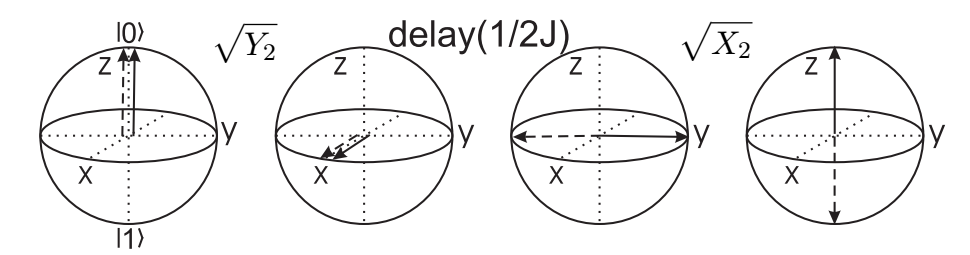
\includegraphics[width=0.7\linewidth]{Figuras/Fig_Harware_NMR_implementacion_CNOT.png}
	\caption{Representación en esfera de Bloch del funcionamiento de la puerta CNOT$_{12}$ entre dos qubits 1 y 2 acoplados por $2 \pi J S_z^1S_z^2/\hbar$ . Aquí se reprensenta el estado del qubit 2 (el qubit objetivo de la CNOT), que comienza en $\ket{0}$ (a lo largo de $\hat{z}$) y se representa en un marco de referencia que gira alrededor de $\hat{z}$ a $\omega_0^2/2 \pi$. Las flechas continuas y discontinuas corresponden al caso en que el qúibit 1 (de controlo) está en $\ket{0}$ y $\ket{1}$ respectivamente. Figura tomada de \cite{bib_NMR_hardware}.}
	\label{Fig_Harware_NMR_implementacion_CNOT}
	\end{figure}

	\Ejercicio{
	Vamos a verificar el paso de la esfera 2 a la 3 de la Fig. \ref{Fig_Harware_NMR_implementacion_CNOT}. Multiplica la matriz de la Ec. (\ref{ec_Hardware_NMR_UJ}) por los dos estados de la segunda esfera de la Fig. \ref{Fig_Harware_NMR_implementacion_CNOT}. Toma $t=1/2J$ y escribe los estados resultantes de la forma \ref{ec_qubit_caso_general} (recuerda que las fases globales no son importantes)
	}
	


El resultado neto es que el espín 2 se invierte si y sólo si el espín 1 está en $\ket{1}$, lo que corresponde exactamente a la tabla de verdad clásica para la CNOT. Las rotaciones $\hat{z}$ adicionales de la Ec. (\ref{ec_Hardware_NMR_implementacion_CNOT}) son necesarias para dar a todos los elementos de $U_{CNOT}$ la misma fase, por lo que la secuencia también funciona para estados de entrada en superposición.

Si el Hamiltoniano de interacción espín-espín no es de la forma $S_z^i S_z^j$ sino que contiene también componentes transversales (como en las Ec. (\ref{ec_Hardware_NMR_H_dipolo-dipolo})), se necesitan otras secuencias de pulsos más complicadas para realizar las puertas CPHASE y CNOT.

Si dos espines no están directamente acoplados entre sí, todavía es posible realizar una puerta CNOT entre ellos, siempre y cuando exista una red de acoplamientos que conecte los dos qubits. Por ejemplo, supongamos que queremos realizar una puerta CNOT con el qubit 1 como control y el qubit 3 como objetivo, CNOT$_{13}$, pero 1 y 3 no están acoplados entre sí. Si ambos están acoplados al qubit 2, como en la red de acoplamiento de la Fig. \ref{Fig_Harware_NMR_posible_couplings}b, podemos primero intercambiar el estado de los qubits 1 y 2 (mediante la secuencia CNOT$_{12}$ CNOT$_{21}$ CNOT$_{12}$, es decir, una puerta SWAP como la de la Fig. \ref{Fig_elementos_Equiv_CNOTs}), luego realizar un CNOT$_{23}$, y finalmente intercambiar de nuevo los qubits 1 y 2. El efecto neto es CNOT$_{13}$. Por extensión, se requieren como máximo $O(n)$ operaciones de intercambio para realizar una CNOT entre cualquier par de qubits en una cadena de $n$ espines con sólo acoplamientos de vecino más cercano (Fig. \ref{Fig_Harware_NMR_posible_couplings}b). Las operaciones SWAP también se pueden utilizar para realizar puertas de dos qubits entre dos qubits cualesquiera que estén acoplados a un qubit ``bus'' común (Fig. \ref{Fig_Harware_NMR_posible_couplings}c).

Por el contrario, si un qubit está acoplado a muchos otros qubits (Fig. \ref{Fig_Harware_NMR_posible_couplings}a) y queremos realizar una CNOT entre sólo dos de ellos, debemos \textbf{eliminar el efecto de los acoplamientos restantes}. Esto se puede lograr utilizando la técnica de \textbf{reenfoque}, que ha sido ampliamente adoptada en una variedad de experimentos de RMN.


	\begin{figure}[H]
	\centering 
	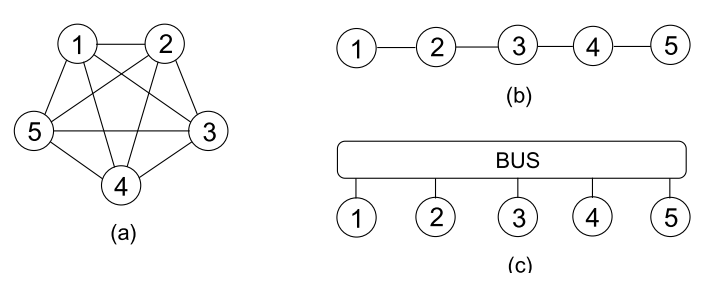
\includegraphics[width=0.65\linewidth]{Figuras/Fig_Harware_NMR_posible_couplings.png}
	\caption{Tres posibles redes de acoplamiento entre cinco qubits. a) Una red de acoplamiento completa. En la práctica, estas redes siempre tendrán un tamaño limitado, ya que las interacciones físicas tienden a disminuir con la distancia. b) Una red de acoplamiento de vecino más próximo. Este tipo de cadenas lineales con acoplamientos de vecino más próximo, o variantes bidimensionales, se utilizan en muchas propuestas de estado sólido. c) Acoplamiento a través de un ``bus''. Es el caso, por ejemplo, de los esquemas de trampas de iones. Al igual que en el caso a), el grado de libertad del bus sólo se acoplará bien a un número finito de qubits. Figura tomada de \cite{bib_NMR_hardware}}
	\label{Fig_Harware_NMR_posible_couplings}
	\end{figure}






			\SubsubiIt{Reenfoque (refocusing): apagando las interacciones $S_z^i S_z^j$ indeseadas} 

Ya hemos visto que al estar los espines acoplados, estos evolucionan con el tiempo siguiendo la Ec. (\ref{ec_Hardware_NMR_UJ}). Si queremos que esta evolución la sientan solo unos ciertos qubits, tenemos que eliminar el efecto de los términos de acoplamiento no deseados. Este es el caso, por ejemplo, de la CNOT. Como ya vimos, el paso intermedio de la CNOT es una evolución libre que solo deben de experimentar los dos qubits implicados en la CNOT. 

El efecto de los términos de acoplamiento durante un intervalo de tiempo de evolución libre puede eliminarse mediante las denominadas técnicas de \textbf{reenfoque}.  Para hamiltonianos de acoplamiento de la forma $S_z^i S_z^j$, como suele ocurrir en los experimentos de RMN de líquidos, el mecanismo de reenfoque puede entenderse a un nivel muy intuitivo. 

Veamos primero dos formas de deshacer $S_z^i S_z^j$ en un sistema de dos qubits. En la Fig. \ref{Fig_Harware_NMR_refocusing}a, la evolución del qubit 1 en el primer intervalo de tiempo $\tau$ se invierte en el segundo intervalo de tiempo, debido al pulso de 180º en el qubit 2. En la Fig. \ref{Fig_Harware_NMR_refocusing}b, el qubit 1 continúa evolucionando en la misma dirección todo el tiempo, pero el primer pulso de 180º hace que los dos componentes del qubit 1 se reenfoquen al final del segundo intervalo de tiempo. El segundo pulso de 180º garantiza que ambos qubits vuelvan siempre a su estado inicial.

Matemáticamente, podemos ver cómo funciona el reenfoque de los acoplamientos $J$ utilizando 
	\begin{equation}
	X_1 \, U_J(\tau) \, X_1 = U_J (- \tau) = X_2 \, U_J \, X_2 \, ,
	\end{equation}
que nos lleva a 
	\begin{equation}
	 X_1 \, U_J(\tau) \, X_1 \, U_J(\tau) = I =  X_2 \, U_J(\tau) \, X_2 \, U_J(\tau)
	\end{equation}

	\Ejercicio{
	Partiendo de los estados de las primeras esferas de Bloch de las figuras  \ref{Fig_Harware_NMR_refocusing}a y \ref{Fig_Harware_NMR_refocusing}b, (sería el estado $\ket{y-}$ de la Ec.    (\ref{ec_qubit_y+})), aplica una a una las puertas de las figuras, comprobando que estas son correctas. (Nota: no hace falta darle un valor a $\tau$, simplemente dejarlo como parámetro libre)
	}



	\begin{figure}[t]
	\centering 
	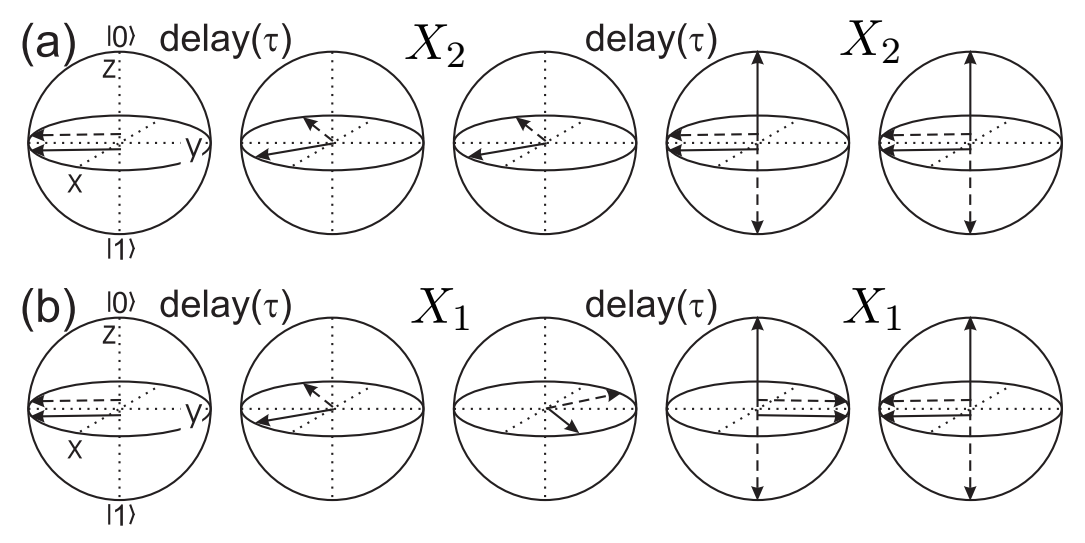
\includegraphics[width=0.7\linewidth]{Figuras/Fig_Harware_NMR_refocusing.png}
	\caption{Representación en esfera de Bloch del funcionamiento de dos esquemas sencillos para reenfocar el acoplamiento entre dos qubits acoplados. El diagrama muestra la evolución del \textbf{qubit 1} (en el sistema rotante) inicialmente a lo largo de $- \hat{y}$, cuando el qubit 2 está en $\ket{0}$ (sólido) o en $\ket{1}$ (discontinuo). Los pulsos de reenfoque puede aplicarse tanto al  qubit 2 (a) como al qubit 1 (b).}
	\label{Fig_Harware_NMR_refocusing}
	\end{figure}


Reemplazando todas las $X_i$ por $Y_i$, las secuencias funcionan igual. Sin embargo, si utilizamos unas veces $X_i$ y otras $Y_i$, obtendremos la matriz identidad salvo algunos desplazamientos de fase. Además, si aplicáramos pulsos en ambos qubits simultáneamente, por ejemplo $X_1X_2 U_J(\tau)X_1 X_2 U_J(\tau)$, el acoplamiento no se eliminaría. 

La Fig. \ref{Fig_Harware_NMR_refocuse_1} da una idea de las técnicas de reenfoque en un sistema multi-qubit. Específicamente, este esquema preserva el efecto de $J_{12}$, mientras que inactiva efectivamente todos los demás acoplamientos. La idea subyacente es que un acoplamiento entre los espines $i$ y $j$ actúa ``hacia delante'' durante los intervalos en los que ambos espines tienen el mismo signo en el diagrama, y actúa ``a la inversa'' siempre que los espines tienen signos opuestos. Cuando un acoplamiento actúa hacia delante y hacia atrás durante el mismo tiempo, no tiene ningún efecto neto.


	\begin{figure}[t]
	\centering 
	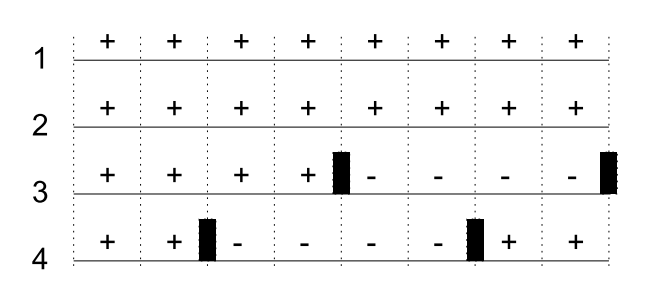
\includegraphics[width=0.5\linewidth]{Figuras/Fig_Harware_NMR_refocuse_1.png}
	\caption{Esquema de reenfoque para un sistema de 4 espines, diseñado para preservar el efecto de la interacción $J_{12}$ todo el tiempo pero neutralizando el efecto del resto de las $J_{ij}$. El intervalo está dividido en segmentos de igual duración, y los signos ``$+$'' y ``$-$'' indican si un espín está en suposición original o del revés. Los rectángulos negros representan pulsos de 180º, que dan la vuelta al correspondiente espín.}
	\label{Fig_Harware_NMR_refocuse_1}
	\end{figure}


Se han desarrollado métodos sistemáticos para diseñar esquemas de reenfoque para sistemas multi-qubit específicamente con el propósito de la computación cuántica. El esquema más compacto se basa en matrices de Hadamard \cite{bib_Hardware_NMR_reenfoque_Hadammard_1}-\cite{bib_Hardware_NMR_reenfoque_Hadammard_2}. Una matriz de Hadamard de orden $n$, denotada por $H(n)$, es una matriz $n \times n$ con entradas $\pm 1$, tal que
	\begin{equation}
	H(n) \, H(n)^T = n I
	\end{equation}
Las filas son, por tanto, ortogonales por pares, y dos filas cualesquiera coinciden exactamente en la mitad de las entradas. Identificando $+1$ y $-1$ con $+$ y $-$ como en el diagrama de la Fig. \ref{Fig_Harware_NMR_refocuse_1}, vemos que $H(n)$ da un esquema de desacoplamiento válido para $n$ espines utilizando sólo $n$ intervalos de tiempo. Un ejemplo de $H(12)$ es
	\begin{equation}
	\begin{bmatrix}
	+ & + & + & + & + & + &  + & + & + & + & + & + \\
	+&+&+&-&-&+&-&-&+&-&-&+\\
	+&+&+&+&-&-&-&+&-&+&-&-\\
	+&-&+&+&+&-&-&-&+&-&+&-\\
	+&-&-&+&+&+&-&-&-&+&-&+\\
	+&+&-&-&+&+&-&+&-&-&+&-\\
	+&-&-&-&-&-&-&+&+&+&+&+\\
	+&-&+&-&-&+&+&-&-&+&+&-\\
	+&+&-&+&-&-&+&-&-&-&+&+\\
	+&-&+&-&+&-&+&+&-&-&-&+\\
	+&-&-&+&-&+&+&+&+&-&-&-\\
	+&+&-&-&+&-&+&-&+&+&-&-\\
	\end{bmatrix}
	\end{equation}

Si queremos que el acoplamiento entre un par de qubits permanezca activo mientras se elimina el efecto de todos los demás acoplamientos, podemos simplemente utilizar la misma fila de $H(n)$ para esos dos qubits. 

$H(n)$ no existe para todos los $n$, pero siempre podemos encontrar una secuencia de desacoplamiento para $n$ qubits tomando las primeras $n$ filas de $H(\bar{n})$, siendo $\bar{n}$ el menor número entero que satisfaga $\bar{n} \geq n $ con $H(\bar{n})$ conocida. A partir de las propiedades de las matrices de Hadamard, podemos demostrar que $\bar{n}/n$ es siempre próximo a 1 (ver \cite{bib_Hardware_NMR_reenfoque_Hadammard_1}). Así que los esquemas de desacoplamiento para $n$ espines requieren $\bar{n}$ intervalos de tiempo y no más de $\bar{n}n$ pulsos de 180º.

Terminamos esta subsección con tres observaciones adicionales.
En primer lugar, cada qubit estará generalmente acoplado a no más de un número fijo de otros qubits, ya que las intensidades de acoplamiento tienden a disminuir con la distancia. En este caso, todos los esquemas de reenfoque pueden simplificarse enormemente. 

En segundo lugar, si las evoluciones hacia delante y hacia atrás bajo
$J_{ij}$ no son iguales en duración, se produce una evolución neta acoplada correspondiente al exceso de evolución hacia delante o hacia atrás. En principio, por tanto, podemos organizar cualquier esquema de reenfoque de forma que incorpore cualquier cantidad deseada de evolución acoplada para cada par de qubits.

En tercer lugar, las secuencias de reenfoque también pueden utilizarse para eliminar el efecto de los términos $S_{z}^i$ en el Hamiltoniano. Por supuesto, estos términos desaparecen en principio si trabajamos en el marco de rotación múltiple (véase la Ec. (\ref{ec_Hardware_NMR_H_sys_control_final_multi_rot})). Sin embargo, puede haber cierta dispersión en las frecuencias de Larmor, por ejemplo debido a inhomogeneidades del campo magnético. Este efecto puede invertirse utilizando pulsos de reenfoque.




% ========================================================
% == Bibliografía

%\newpage
\nocite{*}
\bibliographystyle{ieeetr}
\bibliography{Bibliografia_CICC_UMA}



\end{document}












